
%%%%%%%%%%%%%%%%%%%%%%%%%%%%%%%%%
%% Requirements 
%%%%%%%%%%%%%%%%%%%%%%%%%%%%%%%%%

% (a) Organisation and Presentation of Thesis (i.e. clarity and logical sequence)
% (b) Coverage (i.e. including literature)
% (c) Depth and Quality of research, originality and critical ability shown (i.e scientific hypothesis,
% computational method and validation design, if the conclusion is justifiable by results obtained)

%%%%%%%%%%%%%%%%%%%%%%%%%%%%%%%%%
%% Packages 
%%%%%%%%%%%%%%%%%%%%%%%%%%%%%%%%%

\documentclass[12pt, twoside]{report}
\usepackage[utf8]{inputenc}
\usepackage[a4paper, left=22mm, right=22mm, top=30mm, bottom=25mm]{geometry}
\usepackage{lipsum}
\setlength{\headheight}{15pt}
\linespread{1.25}
\raggedbottom
\usepackage{float}

%% Header and footer formatting
\usepackage{fancyhdr}
\pagestyle{fancy}
\fancyhf{}
\fancyhead[R]{\thepage}
\renewcommand{\chaptermark}[1]{\markboth{#1}{}}
\fancyhead[L]{\chaptername~\thechapter.~\leftmark}
\renewcommand{\headrulewidth}{0pt}

%% TOC
\usepackage[nottoc]{tocbibind}

%% Chapters
\usepackage{titlesec}
\titleformat{\chapter}[display]
{\LARGE\bfseries}{\chaptertitlename~\thechapter}{10pt}{\LARGE}
\titlespacing*{\chapter}{0pt}{-40pt}{10pt}
\titlespacing*{name=\chapter,numberless}{0pt}{-40pt}{10pt}

%% Glossaries
\usepackage[toc, nonumberlist]{glossaries}
\newglossarystyle{modsuper}{%
  \glossarystyle{super}%
  \renewcommand{\glsgroupskip}{}%
  \renewcommand*{\glossaryentryfield}[5]{%
    \glsentryitem{##1}\glstarget{##1}{##2} & ##3\glspostdescription\space ##5\\[5pt]}%
}
\setglossarystyle{modsuper}
\makeglossaries
\loadglsentries{glossaries}
\glsaddall

%% References
\usepackage[sorting=none, style=numeric-comp]{biblatex}
\addbibresource{references.bib}

%% Figures
\usepackage{graphicx}
\graphicspath{{figures/}}
\usepackage{caption}
\usepackage{subcaption}

\usepackage{graphics}

%% Hyperlinks
\usepackage{hyperref}

%% Maths
\usepackage{amsfonts}
\usepackage{amsmath}
\usepackage{amsthm}
\theoremstyle{definition}
\newtheorem{definition}{Definition}[section]
\usepackage{bm}
\newcommand{\ts}{\textsuperscript}
\newcommand{\irow}[1]{% inline row vector
  \begin{smallmatrix}(#1)\end{smallmatrix}%
}
\DeclareMathOperator*{\argmax}{arg\,max}

%% Graphical models
\usepackage{tikz}
\usetikzlibrary{bayesnet}

%% Line numbers
\usepackage[switch, modulo]{lineno}

%% Font
\renewcommand{\familydefault}{\sfdefault} 
\usepackage{caption}
\captionsetup{font=footnotesize}

%% Tables
\usepackage{array}
\newcolumntype{P}[1]{>{\centering\arraybackslash}p{#1}}
\usepackage{bigstrut}

\theoremstyle{definition}
\newtheorem{exmp}{Example}[section]

%% Code
\usepackage{listings}

%% txt include
\usepackage{fancyvrb}
% redefine \VerbatimInput
\RecustomVerbatimCommand{\VerbatimInput}{VerbatimInput}%
{fontsize=\footnotesize,
 frame=lines,  % top and bottom rule only
 framesep=2em, % separation between frame and text
 label=manual,
 labelposition=topline,
 commentchar=*        % comment character
}

%%%%%%%%%%%%%%%%%%%%%%%%%%%%%%%%%
%% Document starts here
%%%%%%%%%%%%%%%%%%%%%%%%%%%%%%%%%

\begin{document}

\pagenumbering{gobble}


\begin{titlepage}
   \begin{center}
       \vspace*{1cm}
       
       \Large
       \textbf{Statistical models for transcript quantification from long-read RNA-seq}
       
       \vspace{1.5cm}
       
       \large
       by\\
       
       \vspace{0.25cm}
       
       Joseph Lee Jing Xian
       
       \vspace{1.5cm}
       
       Honours Project in Computational Biology
       
       \vspace{0.25cm}
       
       Faculty of Science
       
       \vspace{0.25cm}
       
       National University of Singapore
       
       \vspace{1.5cm}
       
       Supervisor:
       
       \vspace{0.25cm}
       
       Dr. Jonathan Göke
       
       \vspace{0.25cm}
       
       Genome Institute of Singapore
       
       \vspace{1.5cm}
       
       Co-supervisor:
       
       \vspace{0.25cm}
       
       Prof. Greg Tucker-Kellogg
       
       \vspace{0.25cm}
       
       National University of Singapore
       
       \vfill
       
       May 2022

   \end{center}
\end{titlepage}

\chapter*{Abstract}

Long-read RNA-seq technologies have enabled the profiling of full-length reads while mitigating biases in previous generations of RNA-seq technologies, improving the accuracy of isoform abundance estimates. However, biases present in long-read RNA-seq data and their effects on transcript quantification have not yet been extensively explored in the literature.\\[10pt] 
In this thesis, we examine \textit{degradation bias} present in long-read direct RNA-seq, where reads are truncated and map to multiple isoforms, leading to ambiguity in read-to-isoform assignment and erroneous isoform abundance estimates. We characterise degradation in real datasets, develop a bias-aware model for transcript quantification and derive statistical methods for inferring isoform abundance estimates. By accounting for degradation bias, we demonstrate improvements in transcript quantification on simulated datasets with known degradation rates and real datasets with sequencing spike-ins.



%\chapter*{Acknowledgements}
%
I thank Jonathan Göke for conceptualising this work and granting me the opportunity to work on it. I also thank him for his continual guidance, not only for the duration of this thesis, but also from the time I joined his lab in the summer of 2020. His support and patience have been invaluable.\\[10pt]
My gratitude extends also to Chen Ying and Andre Sim for their contributions to this work. The weekly discussions on this subject, the resources they have provided, and the suggestions they have given me have all shaped this work crucially.\\[10pt] 
Further thanks to all members of Jonathan's lab, whom have sat through presentations on this work and have asked questions and provided comments that have been useful. Their work is brilliant, and has given me much insight and piqued my interest in all things long-read.\\[10pt]
I also thank Prof. Greg Tucker-Kellogg for his co-supervision and for conducting great courses in bioinformatics at NUS that have laid foundations instrumental to this work.\\[10pt] 
Last but not least, I thank Prof. Choi Hyungwon for a large part of my statistical education, which has come to fruition in this work.  

\tableofcontents

\pagenumbering{roman}

\listoffigures

\listoftables

\printglossaries

\chapter{Introduction}
\pagenumbering{arabic}

Third generation sequencing technologies have enabled the production of long reads ranging from tens to hundreds of kilobases in length \cite{Pollard2018}, and have shown promise in resolving many challenges in genomics and transcriptomics \cite{Bolisetty2015, Byrne2017, DeCoster2019, Liu2019, Mantere2019, Nurk2021}. In particular, long-read technologies enable greater insight into the transcriptome and its complexity, which is crucial in understanding the functioning of cells and their biological processes. These technologies allow accurate detection of a larger proportion of full-length transcripts and novel splice junctions while mitigating biases associated with short-read technologies, enabling more accurate abundance estimates of reference and novel isoforms. Nevertheless, biases are still present in long-read technologies, albeit to a lesser extent. 

This thesis focuses on a particular bias present in long-read direct RNA-seq referred to as \textit{degradation bias}. This bias arises due to the fact that from the time a transcript is generated to when it is sequenced, it is subject to multiple factors that results in its degradation. Consequently, the reads obtained from sequencing are often truncated, resulting in ambiguity in read assignment to transcript isoforms. This, in turn, leads to erroneous isoform abundance estimates. 

In this thesis, we attempt to characterise degradation bias and its effects on quantification from long-read direct RNA-seq, and develop a framework to model and correct such bias for accurate transcript quantification and isoform abundance estimation.

\section{Review}

Here, we review various concepts and existing literature relevant to our aim of modeling bias in long-read RNA-seq. We first examine (i) biases in short-read RNA-seq technologies and how they are accounted for by existing methods, which provide useful ideas on how to handle biases in long-read RNA-seq. Next, we review (ii) long-read RNA-seq technologies and how they mitigate biases in (i), and (iii) biases that long-read technologies themselves possess. 

\subsection{Bias modeling in short-read RNA-seq}

Short-read RNA-seq technologies enable deep sequencing of highly accurate short reads, and has been the dominant technology for profiling the transcriptome since its popularisation in the early 2010s \cite{Lowe2017}. Typically, library preparation protocol for an RNA-seq experiment following \gls{rna} extraction involves \gls{rna} fragmentation, followed by the use of random hexamer primers for priming of the fragments to synthesize one strand of \gls{cdna}. After second strand synthesis, the resulting double stranded \gls{cdna} are size-selected and amplified via \gls{pcr} amplification to generate enough \gls{cdna} for sequencing \cite{Marguerat2010}.  

Biases in short-read RNA-seq have been extensively studied \cite{Hansen2010, Li2010, Li2011, Zhengpeng2010, Roberts2011, Benjamini2012, Lahens2014, Love2016}, and can often be traced back to specific steps in the protocol described above. For instance, \cite{Hansen2010} showed that priming with random hexamer primers induces bias in the nucleotide composition of the reads and results in non-uniform representation of reads across the length of the transcript. In addition, size selection of fragments results in an over-representation of fragments of a certain length, while \gls{rna} degradation and \gls{mrna} selection can lead to over-representation of fragments that are located towards either the beginning or end of the transcript \cite{Roberts2011, Lahens2014, Love2016}. \gls{pcr} amplification before sequencing also introduces bias by preferential amplification of fragments with certain GC content \cite{Benjamini2012, Love2016}. The combination of these biases affect quantification estimates, and if not corrected for, leads to erroneous estimates \cite{Roberts2011, Love2016}. 

Existing methods to address these biases can be categorised into two broad classes. The first class of methods involve innovations in library preparation methods to reduce bias from their source of origin \cite{Vandijk2014}. For instance, an amplification-free RNA-seq protocol was proposed in \cite{Mamanova2010} to reduce amplification bias, while thermostable polymerases that exhibit relatively lower GC bias were identified in \cite{Quail2012}. We focus on the second class of methods that involve modeling and correcting for the bias \textit{in silico}. In particular, we focus on the approaches in the literature that are most relevant to our aim. 

% Single-isoform genes
In modeling bias, one needs to estimate parameters describing the bias from the data. The first approach adopted by many short-read RNA-seq methods for modeling bias is to use single isoform genes for estimating bias parameters. For instance, 
Cufflinks corrects for fragment length bias by estimating fragment length distributions based on a set of single isoform gene \cite{Roberts2011}, while alpine  estimates bias offsets and coefficients from single isoform genes for fragment length, read start sequence preference and GC content \cite{Love2016}. This approach ensures that the bias terms are computed from a subset of the data with the least ambiguity in assignment to the correct isoform. Furthermore, due to the complexity in real data, non-parametric density estimation is often used to model certain features. Again, both Cufflinks and alpine use kernel density estimates to fit an empirical fragment length distribution to correct for positional bias, i.e., the enrichment of fragments at the start or end of the transcripts. RSEM uses an empirical distribution to model the position of reads within fragments \cite{Li2011}. Other complex parametric approaches have been used, such as a mixture of Gaussian in \cite{MIXMIX}, but appear less popular possibly due to parametric constraints. Last and perhaps most relevant is the use of curves to characterise and model for bias. In \cite{NURD}, coverage over single isoform genes is used to compute global and local bias curves which are then used to describe the non-uniformity of read distributions across all genes and for each gene respectively. In particular, the coverage over a gene is binned and transformed into a step function over exons of a gene \cite{NURD}. We consider all these approaches when characterising bias and modeling for it in the following chapters. 

\subsection{Long-read technologies}

As the name suggests, long-read sequencing technologies allow the sequencing of long reads ranging from one to hundreds of kilobases, improving over short-read technologies that yield fragments ranging from 50 to 600 bp. This has been made possible by the development of biophysical techniques to capture full-length DNA and RNA \cite{Weirather2017}. While the increased read length provided by these technologies has enabled leaps in genomics and transcriptomics research \cite{Bolisetty2015, Byrne2017, DeCoster2019, Liu2019, Mantere2019, Nurk2021}, these same technologies suffer from high sequencing error rates and low throughput \cite{Carneiro2012, Reuter2015, Jain2015}.  

Two of the most widely used platforms for long-read sequencing include Pacific Biosciences (PacBio) and Oxford Nanopore Technologies (ONT). We omit discussion on PacBio data for the time being as we work only with ONT data in this thesis. ONT is a nanopore-based sequencing technology that currently provides three protocols for transcriptomic sequencing: direct RNA, direct cDNA and PCR-cDNA sequencing. In all three protocols, DNA or RNA is processed and ligated with sequencing adaptors comprising a motor protein that ensures unidirectional single-nucleotide translocation through the nanopore on the order of milliseconds \cite{Jain2016}. Each nanopore is associated with a sensor that measures changes in ionic current caused by differences in the nucleotides occupying the pore \cite{Jain2016}, giving rise to raw electric current signal. In addition, the nanopores are embedded in a synthetic electrically-resistant membrane to ensure that all current only passes through the pore, resulting in a cleaner signal \cite{Wang2021}. The raw electric current signal is then translated to nucleotide sequence via base-calling algorithms \cite{Rang2018}. 

We briefly describe the similarities and differences between the three ONT protocols, with a focus on direct RNA-seq. In direct RNA-seq (Fig. \ref{fig:sec-1-drna}), native poly(A) RNA molecules are enriched and directly sequenced from the 3' end. An optional reverse transcription step stabilizes the RNA strand by reducing intramoleulcar secondary structure of the RNA, resulting in better sequencing output \cite{Garalde2018}. In direct cDNA and PCR-cDNA protocols, poly(A) RNA is reverse transcribed followed by second strand synthesis to produce double stranded cDNA. Strand-switching is used to increase the proportion of full-length cDNAs. In PCR-cDNA, double stranded cDNAs are amplified prior to sequencing, giving higher throughput. Across all three protocols, GC bias was evaluated to be minimal in the data, including data from the PCR-cDNA protocol, provided that the number of PCR cycles was capped \cite{ONT}. 

Compared to cDNA protocols, direct RNA-seq mitigates any form of bias or errors due to PCR or reverse transcription \cite{Garalde2018, Depledge2019} which is important for obtaining accurate and reliable isoform abundance estimates. Despite this, a recent evaluation of ONT direct RNA-seq showed that although direct RNA-seq yielded significantly longer reads compared to short-read RNA-seq, the proportion of reads corresponding to full-length transcripts remained low due to read truncation \cite{Soneson2019}. Assigning direct RNA-seq reads to their isoform of origins remains highly nontrivial, in large part due to the number of secondary alignments for each read \cite{Soneson2019}. In the following section, we review some possible explanations for the observed read truncation.   

\begin{figure}[H]
    \centering
    \includegraphics[width=\textwidth]{figures/sec-1-drna.png}
    \caption[ONT direct RNA-sequencing protocol]{ONT direct RNA-sequencing protocol. \textbf{a.} Native RNA with 3' poly(A) tails are enriched for sequencing. poly(A) tails can be added to non-poly(A) RNA with a poly(A)-tailing kit. \textbf{b.} A poly(T) adaptor is annealed to native RNA to prime first-strand synthesis of cDNA. \textbf{c.} Reverse transcription of the RNA strand stabilises it for sequencing and improves sequencing output. \textbf{d.} A sequencing adaptor comprising a motor protein is ligated to the RNA strand and is necessary for guiding it through the nanopore. \textbf{e.} RNA traverses through the nanopore, producing raw signal output which is then basecalled.}
    \label{fig:sec-1-drna}
\end{figure}

\subsection{Biases in long-read RNA-seq}

We now discuss biases in long-read ONT data with a particular focus on degradation bias observed in the direct RNA protocol.

\paragraph{GC bias} According to ONT, datasets sequenced with all three protocols (direct RNA, direct cDNA, PCR cDNA) exhibit virtually no GC bias \cite{ONTGC}, with low correlations between the GC content and read count for each gene. This was corroborated by studies finding that compared to other high throughput sequencing methods such as short-read RNA-seq or PacBio sequencing, there was no relative coverage biases across regions of different GC content \cite{Nookaew2017, HTSGC}. 

\paragraph{Degradation bias} Here, we consider sources of degradation bias observed in long-read direct RNA-seq, where the reads are degraded or truncated \cite{Soneson2019, Workman2019}. This results in ambiguity in read-to-isoform assignment \cite{Soneson2019} (Fig. \ref{fig:degbias}). 

Broadly, factors that influence transcript degradation can be broadly classified as being intra-cellular (\textit{in vivo}) or extra-cellular (\textit{in vitro}). We first examine the dominant source of degradation \textit{in vivo}, which is RNA decay. RNA decay is a well studied phenomena, and can occur due to the action of both exo- and endoribonucleases \cite{CONTI2005, Garneau2007, HOUSELEY2009, Keene2010}. In the first instance, RNA decay occurs due to exoribonuclease cleavage from the 5’ or 3’ ends of the transcript. In mRNAs, this results in the removal of modifications such as 5’-capping or 3’-polyadenylation that help to stabilise the transcript for translation initiation, initiating RNA degradation. Such degradation can occur in both the 5’-3’ or 3’-5’ directions, with the former being the more dominant pathway \cite{Garneau2007}.  

\begin{figure}[H]
    \centering
    \includegraphics[width=\textwidth]{figures/sec-1-degbias.png}
    \caption[Degradation bias results in multi-mapping reads]{Degradation bias results in multi-mapping reads. In this hypothetical scenario, there are three isoforms transcribed (blue, green, red). Their transcripts are sequenced to produce reads (orange). Due to degradation, the observed reads are truncated, predominantly from the 5' end. This results in multi-mapping reads (starred). The number of possible isoforms each read is compatible with is indicated by the number of stars adjacent to the read.}
    \label{fig:degbias}
\end{figure}

A minor pathway for RNA decay involves endoribonuclease cleavage within the body of the transcript \cite{Garneau2007}. Endoribonuclease cleavage within the transcript body exposes unprotected 5’ and 3’ ends of the distal and proximal segments of the cleaved transcript, which then expose these segments to degradation by exoribonucleases \cite{ Gatfield2004,Garneau2007}. Differential rates of mRNA decay in different functional sets of genes have also been studied. For instance, transcription factor mRNAs tend to exhibit higher rates of mRNA decay compared to mRNA that code for proteins \cite{Yang2003}. Other classes of RNA also exhibit variable decay patterns \cite{Keene2010}; \cite{Kaiwan2021} described large variability in the decay rates of lncRNA compared to mRNAs, finding lncRNAs that were both extremely short-lived and long-lived. 

Compared to \textit{in vivo} effects, extra-cellular \textit{in vitro} effects are less well studied, due to the relative novelty of nanopore sequencing. In \cite{Workman2019}, it was suggested that read truncation in nanopore sequencing could be due to electronic signal noise from current spikes of unknown origin. In addition, pore blocking, which results in the stoppage of RNA translocation through the nanopore, could also result in truncated reads \cite{Amarasinghe2020}. Besides these considerations, generic factors that are not specific to nanopore sequencing, such as the fragmentation of transcripts during library preparation, can also result in the observed read truncation. Bearing in mind these sources of degradation, we aim to characterise biases observed in direct RNA-seq datasets, and model and correct for degradation bias to obtain accurate isoform abundance estimates. 

\section{Organisation}

The chapters of this thesis are organised as follows:
\begin{itemize}
    \item In Chapter 2, we formalise the notion of degradation, and characterise degradation in long-read direct RNA-seq data in reference isoforms and sequencing spike-ins across multiple cell lines and samples. 
    \item In Chapter 3, we develop a generative model for degradation-aware transcript quantification and derive expectation maximization and variational inference algorithms for parameter inference. 
    \item In Chapter 4, we evaluate our model and inference algorithms on simulated datasets with known degradation and real datasets with sequencing spike-ins. We benchmark our model against existing long-read transcript quantification methods in the literature. 
    \item In Chapter 5, we summarise the ideas of this thesis and discuss potential directions of future work. 
\end{itemize}

\chapter{Characterising degradation}

In this chapter, we aim to characterise transcript degradation and read truncation from long-read RNA-seq data. Transcript degradation from the 5' end results in truncated reads and a decrease in coverage with increasing distance from the 3' end for a given isoform. Thus, even though the observed degradation occurs from the 5' end, it is helpful to characterise degradation as the resultant decrease in coverage from the 3' end. We formalize the notion of degradation by defining the \textit{degradation rate}. 
\begin{definition}[Normalized coverage]
Let the maximum coverage over an isoform be $\mathrm{cov}_{\mathrm{max}}$ and the coverage at base $b$ be $\mathrm{cov}_b$. The normalized coverage of the isoform at base $b$ is defined as 
\begin{equation}
    \mathrm{ncov}_b=\frac{\mathrm{cov}_b}{\mathrm{cov}_{\mathrm{max}}}
\end{equation}
\end{definition}
\begin{definition}[Degradation rate]
Let $\mathrm{ncov}$ be the normalized coverage over an isoform, and $x$ be the distance in kb from the 3' end. The degradation rate of an isoform is defined as the rate of change in normalized coverage with respect to distance in kb from the 3' end of the isoform:
\begin{equation}
    d=\lim_{\Delta x\rightarrow 0} \frac{\Delta \mathrm{ncov}}{\Delta x}
\end{equation}
The degradation rate of an isoform at a base $b$ with distance $x_b$ away from the 3' end is the value of this limit evaluated at $x=x_b$. 
\end{definition}
Intuitively, the degradation rate can be interpreted as the gradient of the plot of normalized coverage against distance from the 3' end. We will refer to this plot as the \textbf{degradation curve}. To illustrate this, we visualise degradation curves for a hypothetical isoform of length 2 kb with different degradation rates (Fig. \ref{fig:sec-2-hypo}).  
\begin{figure}[H]
    \centering
    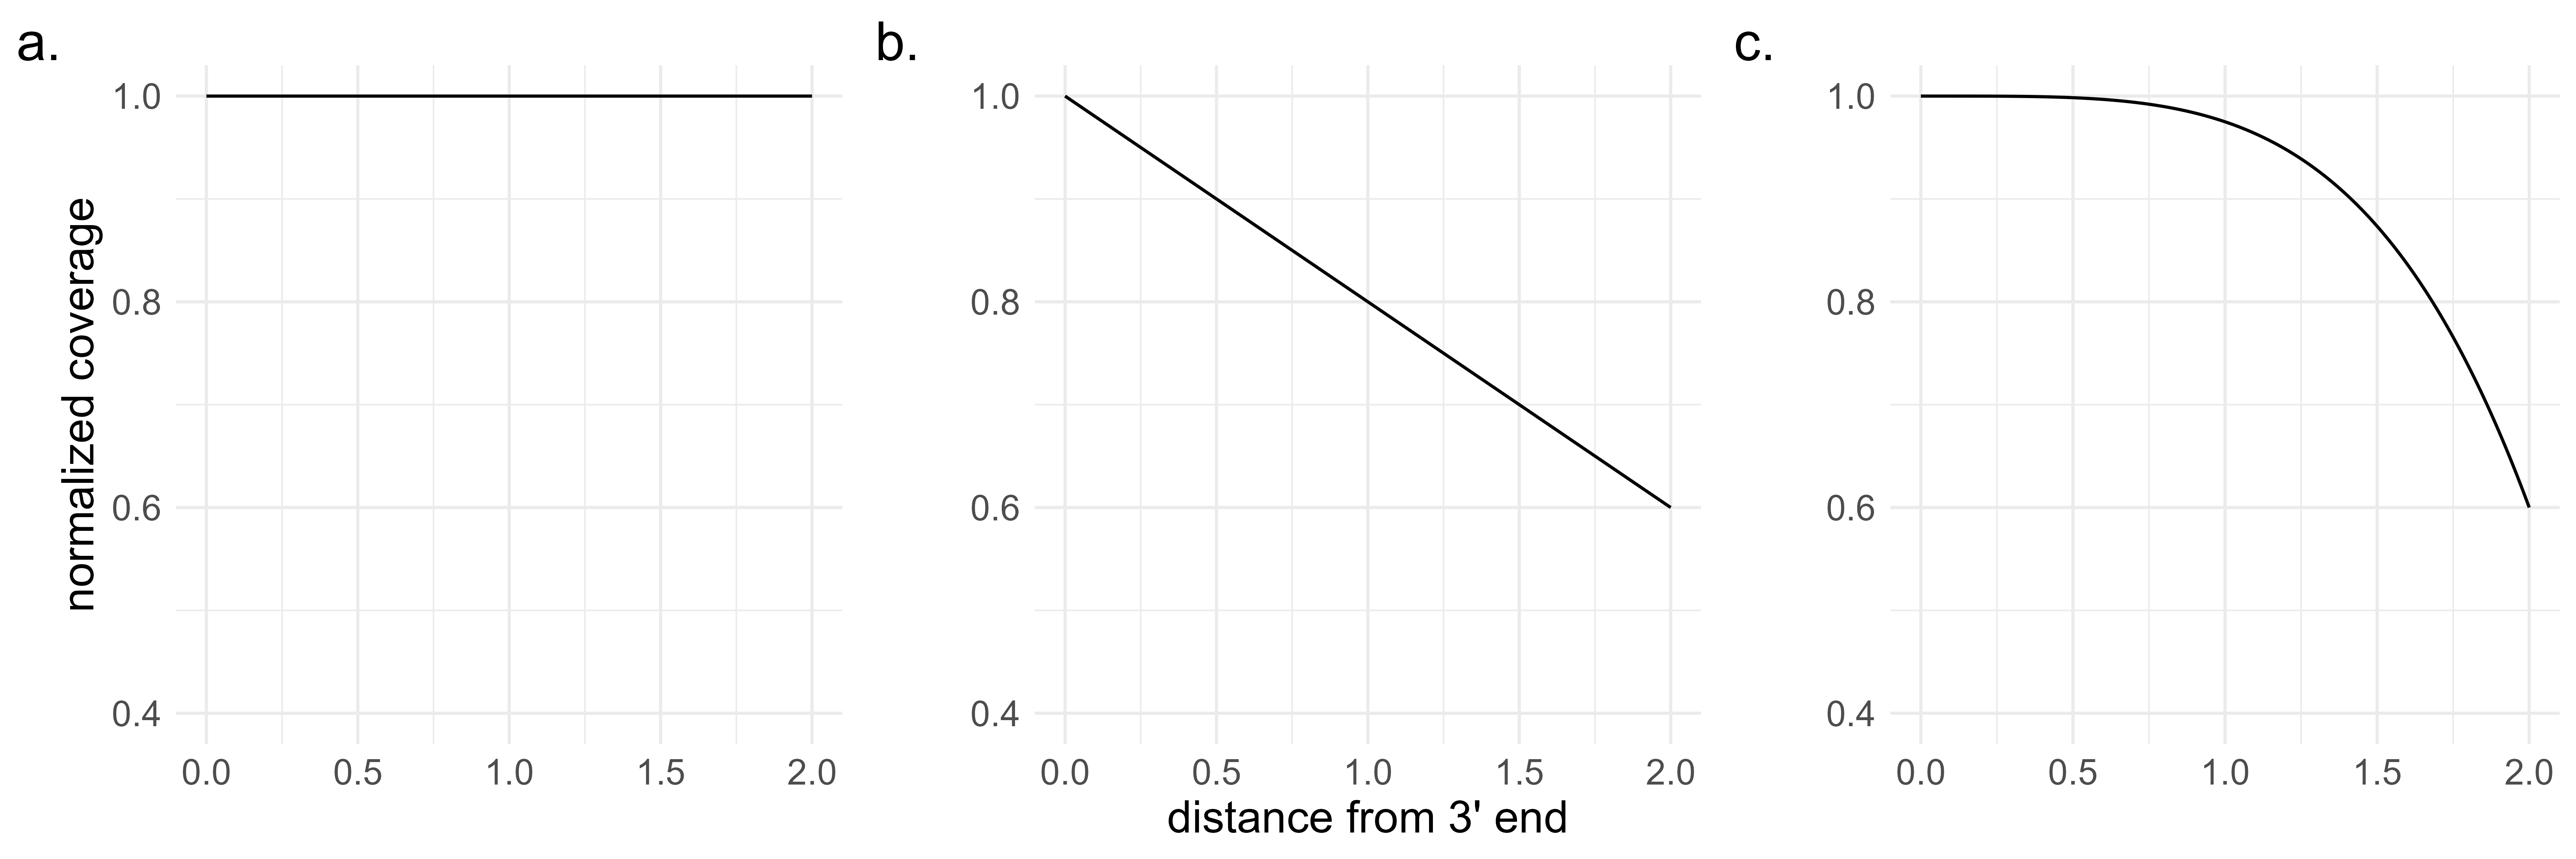
\includegraphics[width=\textwidth]{figures/sec-2-hypo.png}
    \caption[Normalized coverage plots for a hypothetical isoform]{Normalized coverage plots for a hypothetical isoform of length 2 kb illustrating different degradation rates. \textbf{a.} Degradation rate is 0. \textbf{b.} Degradation rate is constant (0.2). \textbf{c.} Degradation rate is variable.}
    \label{fig:sec-2-hypo}
\end{figure}
In Fig. \ref{fig:sec-2-hypo}a, the degradation rate or gradient is 0, implying that all reads from the isoform are full-length, with no drop in coverage over the isoform body. Conversely, in Fig. \ref{fig:sec-2-hypo}b, the gradient is a constant value of 0.2 over the isoform body, implying that for every 1 kb from the 3' end, normalized coverage drops by 0.2. The last plot in Fig. \ref{fig:sec-2-hypo}c shows variable gradient over the isoform body. In particular, the gradient is low in magnitude towards the 3' end and increases with distance from the 3' end.  

In the following sections, we first describe a coverage-based approach for characterising degradation in long-read direct RNA-seq data, and validate this approach with simulated data where the degradation is known. We then examine degradation in real data, characterising degradation by isoform features and in sequencing spike-ins. Finally, we develop a method for efficient read length-based degradation estimation that can be used for obtaining degradation-aware isoform abundance estimates.

\section{Coverage-based degradation estimation}\label{sec:deg-est}

We first sought to determine if patterns of degradation were consistent across transcript isoforms for a given direct RNA-seq dataset. To that end, we selected single-isoform, multi-exon genes from GRCh38 reference annotations, and further restricted the set of isoforms to those that do not intersect with any other annotated features in reference annotations. We refer to these as \textbf{lone isoforms}. Estimating bias from lone isoforms reduces ambiguity in the isoform of origin of the reads we use to estimate bias; such approaches were also adopted in \cite{Roberts2011} and \cite{Love2016} for bias estimation in short-read data. Filtering yielded approximately 5,000 lone isoforms. For each of these isoforms, we obtained coverage over the isoform body using the \texttt{genomecov} module from bedtools (v.2.27.1). Next, we further apply a median coverage filter, filtering out lone isoforms with low median coverage (min median coverage = 10). Finally, a degradation curve is fitted to the data with a smoothing spline.  

To validate this approach, we simulated two datasets where the expected degradation rates for all isoforms is constant ($\mathbb{E}[d]\in\{0.2,0.4\}$, see Appendix \ref{ap:sim-deg-reads} for more details on degraded read simulation). Visualising the degradation curves for each isoform, we observed noise in the form of deviation from the expected degradation curve, likely due to sampling noise in the simulation data generation process. This noise can be mitigated by computing a global degradation curve across all isoforms (red line, Fig. \ref{fig:cov-sim}). We find that the global degradation curves reflect the known degradation rates from the simulated data qualitatively (Fig. \ref{fig:cov-sim}). In addition, we assessed the global degradation curves quantitatively by computing the average gradients of each curve, and found good agreement between the estimates and the expected degradation ($\mathbb{E}[d]$ = 0.2, estimated = 0.201; $\mathbb{E}[d]$ = 0.4, estimated = 0.403).

We applied this approach in real direct RNA-seq data from the SG-NEx project. Within each sample, we found consistent patterns of degradation across isoforms (Fig. \ref{fig:cov-real}). However, we note that for most real datasets, filtering for lone transcripts and by median coverage yields very few isoforms remaining for estimating degradation rates. For instance, in a HepG2 sample (Fig. \ref{fig:cov-real}a), we obtained only 57 isoforms, while in a MCF7 sample (Fig. \ref{fig:cov-real}b), we obtained only 52 isoforms. Across the samples, the median number of lone isoforms post-filtering was 21. While this approach separates signal and noise by considering only lone isoforms, it may be overly restrictive. We consider an improved approach for estimating the degradation rate in Section \ref{sec:rld} based on observed read length distributions. 

\begin{figure}[H]
    \centering
    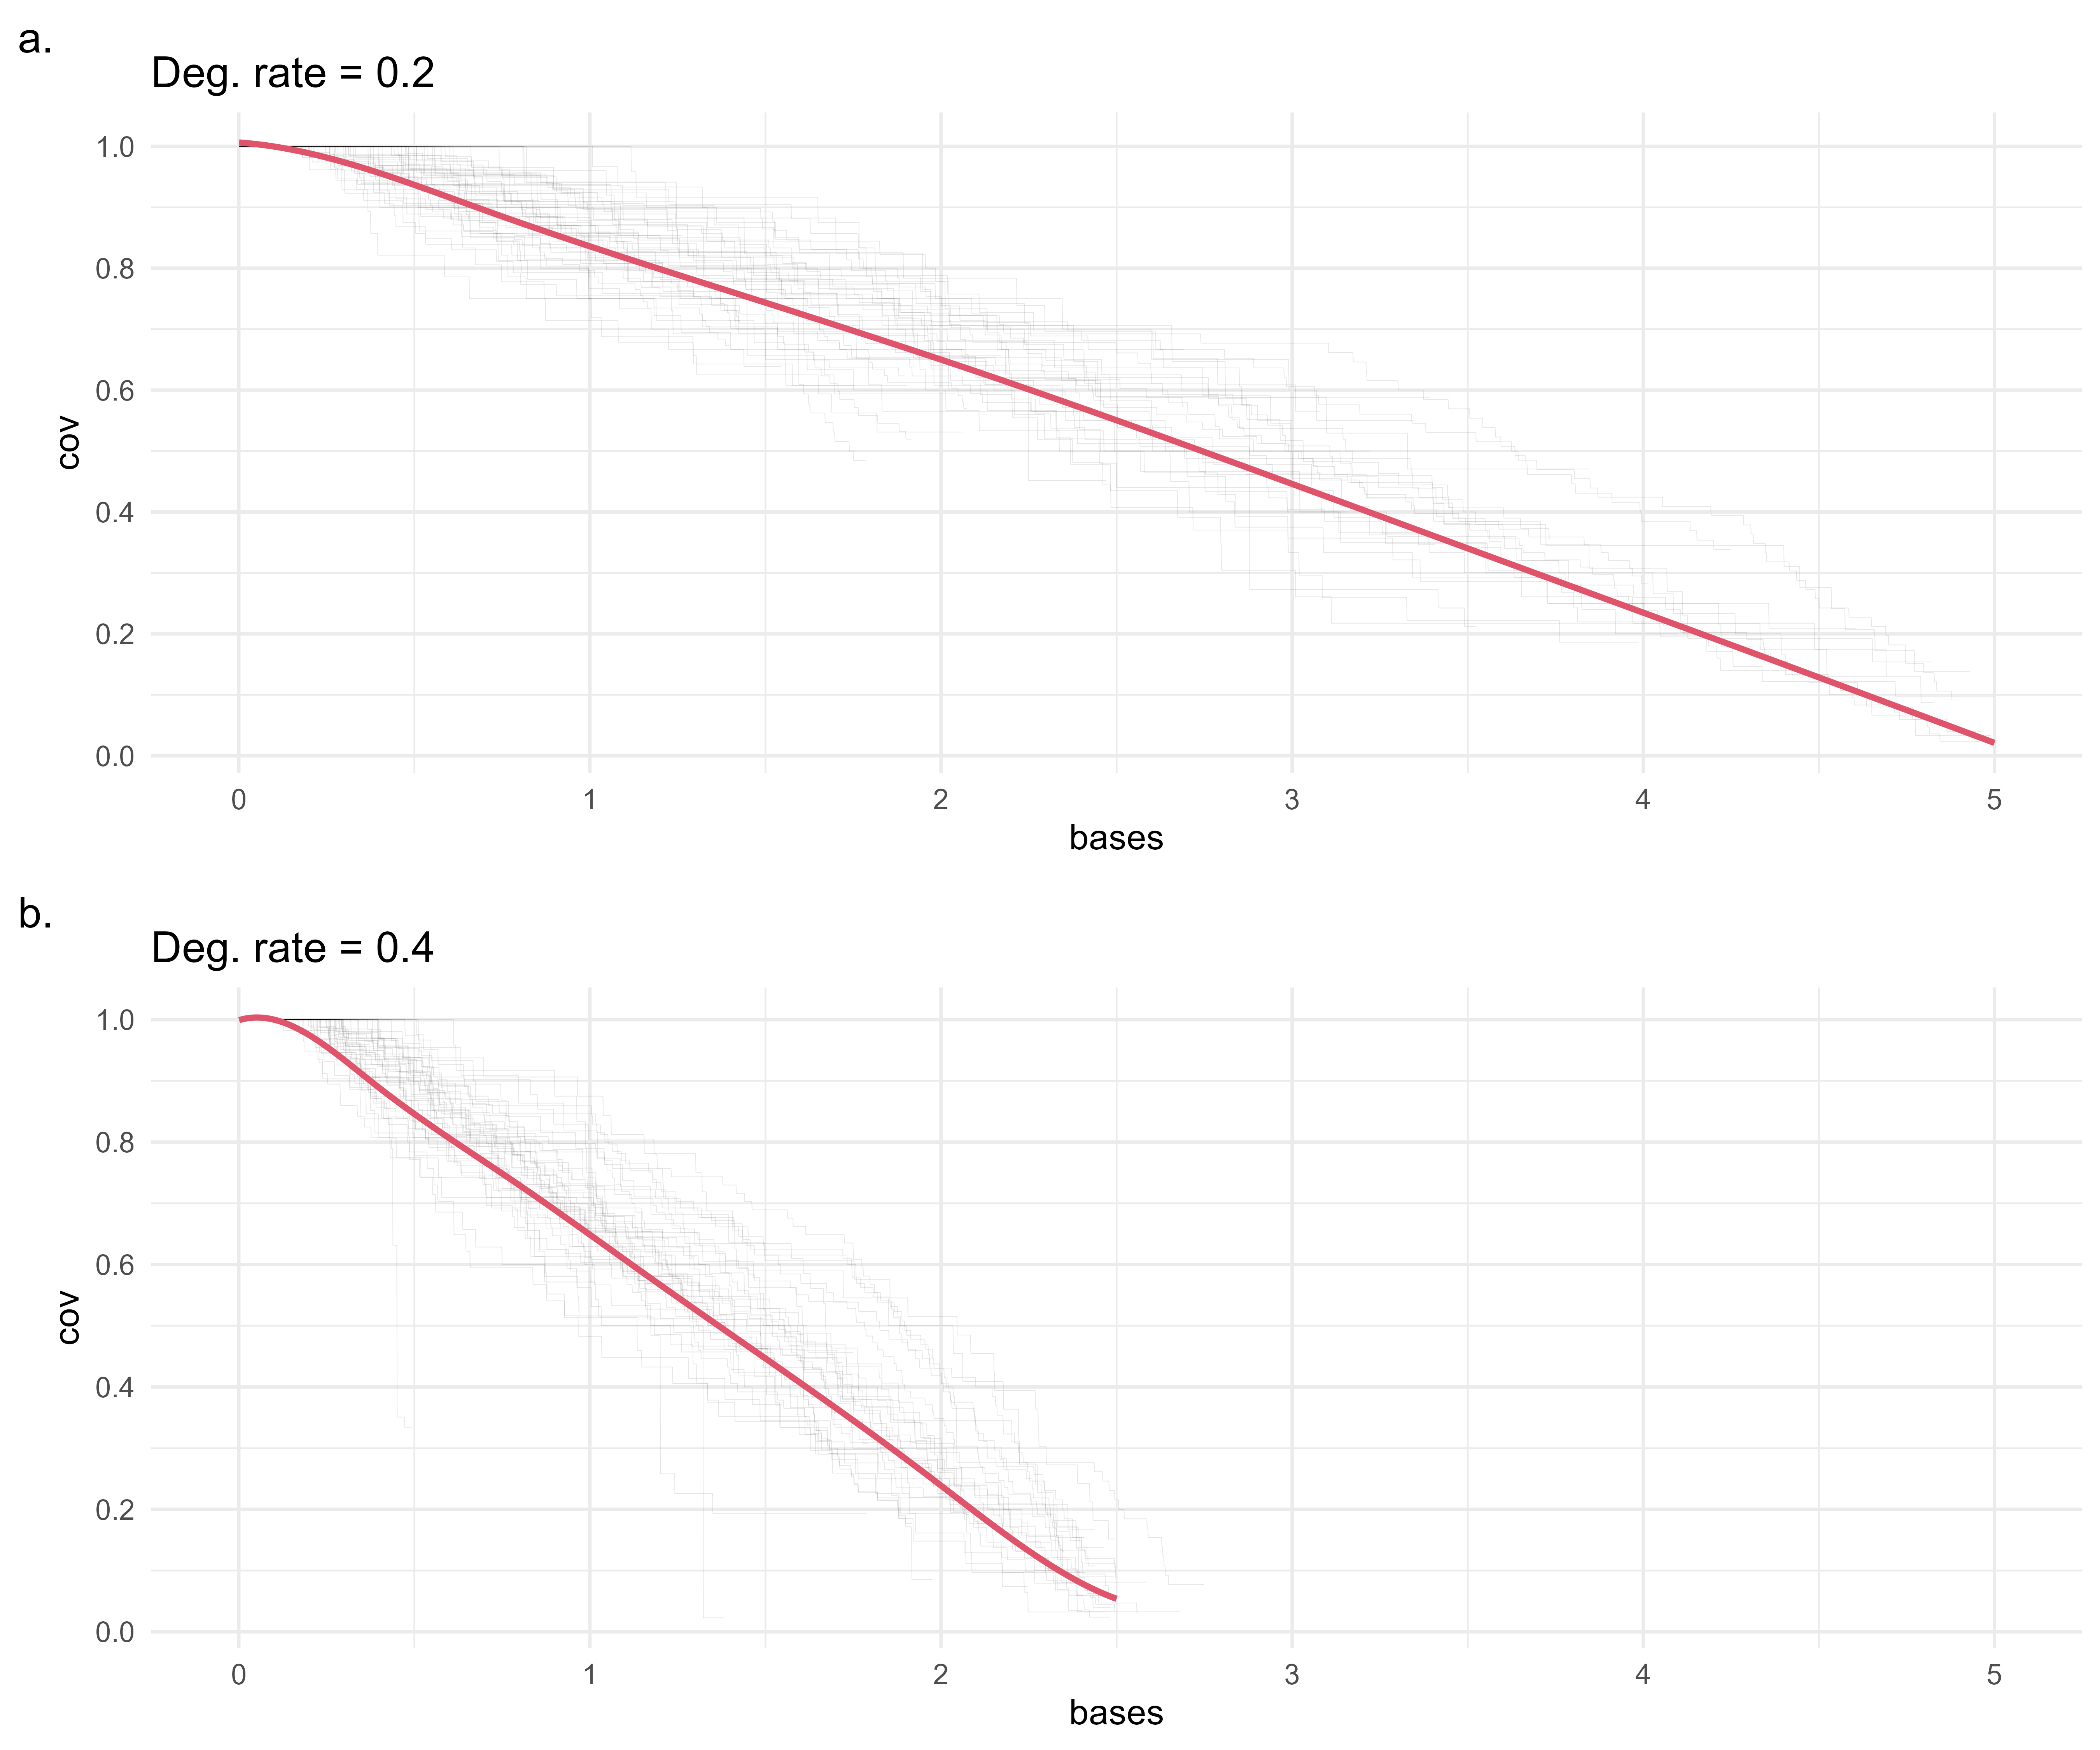
\includegraphics[width=0.9\textwidth]{figures/sec-2-cov-sim.png}
    \caption[Degradation curves on simulation datasets based on coverage]{Degradation curves on simulation datasets based on coverage. \textbf{a.} Degradation curve for dataset with $\mathbb{E}[d]$ = 0.2. Coverage drops close to 0 at 5kb with a degradation rate of 0.2. The estimated degradation rate is 0.201. \textbf{a.} Degradation curve for dataset with $\mathbb{E}[d]$ = 0.4. Coverage drops close to 0 at 2.5 kb. The estimated degradation rate is 0.403.}
    \label{fig:cov-sim}
\end{figure}

\begin{figure}[H]
    \centering
    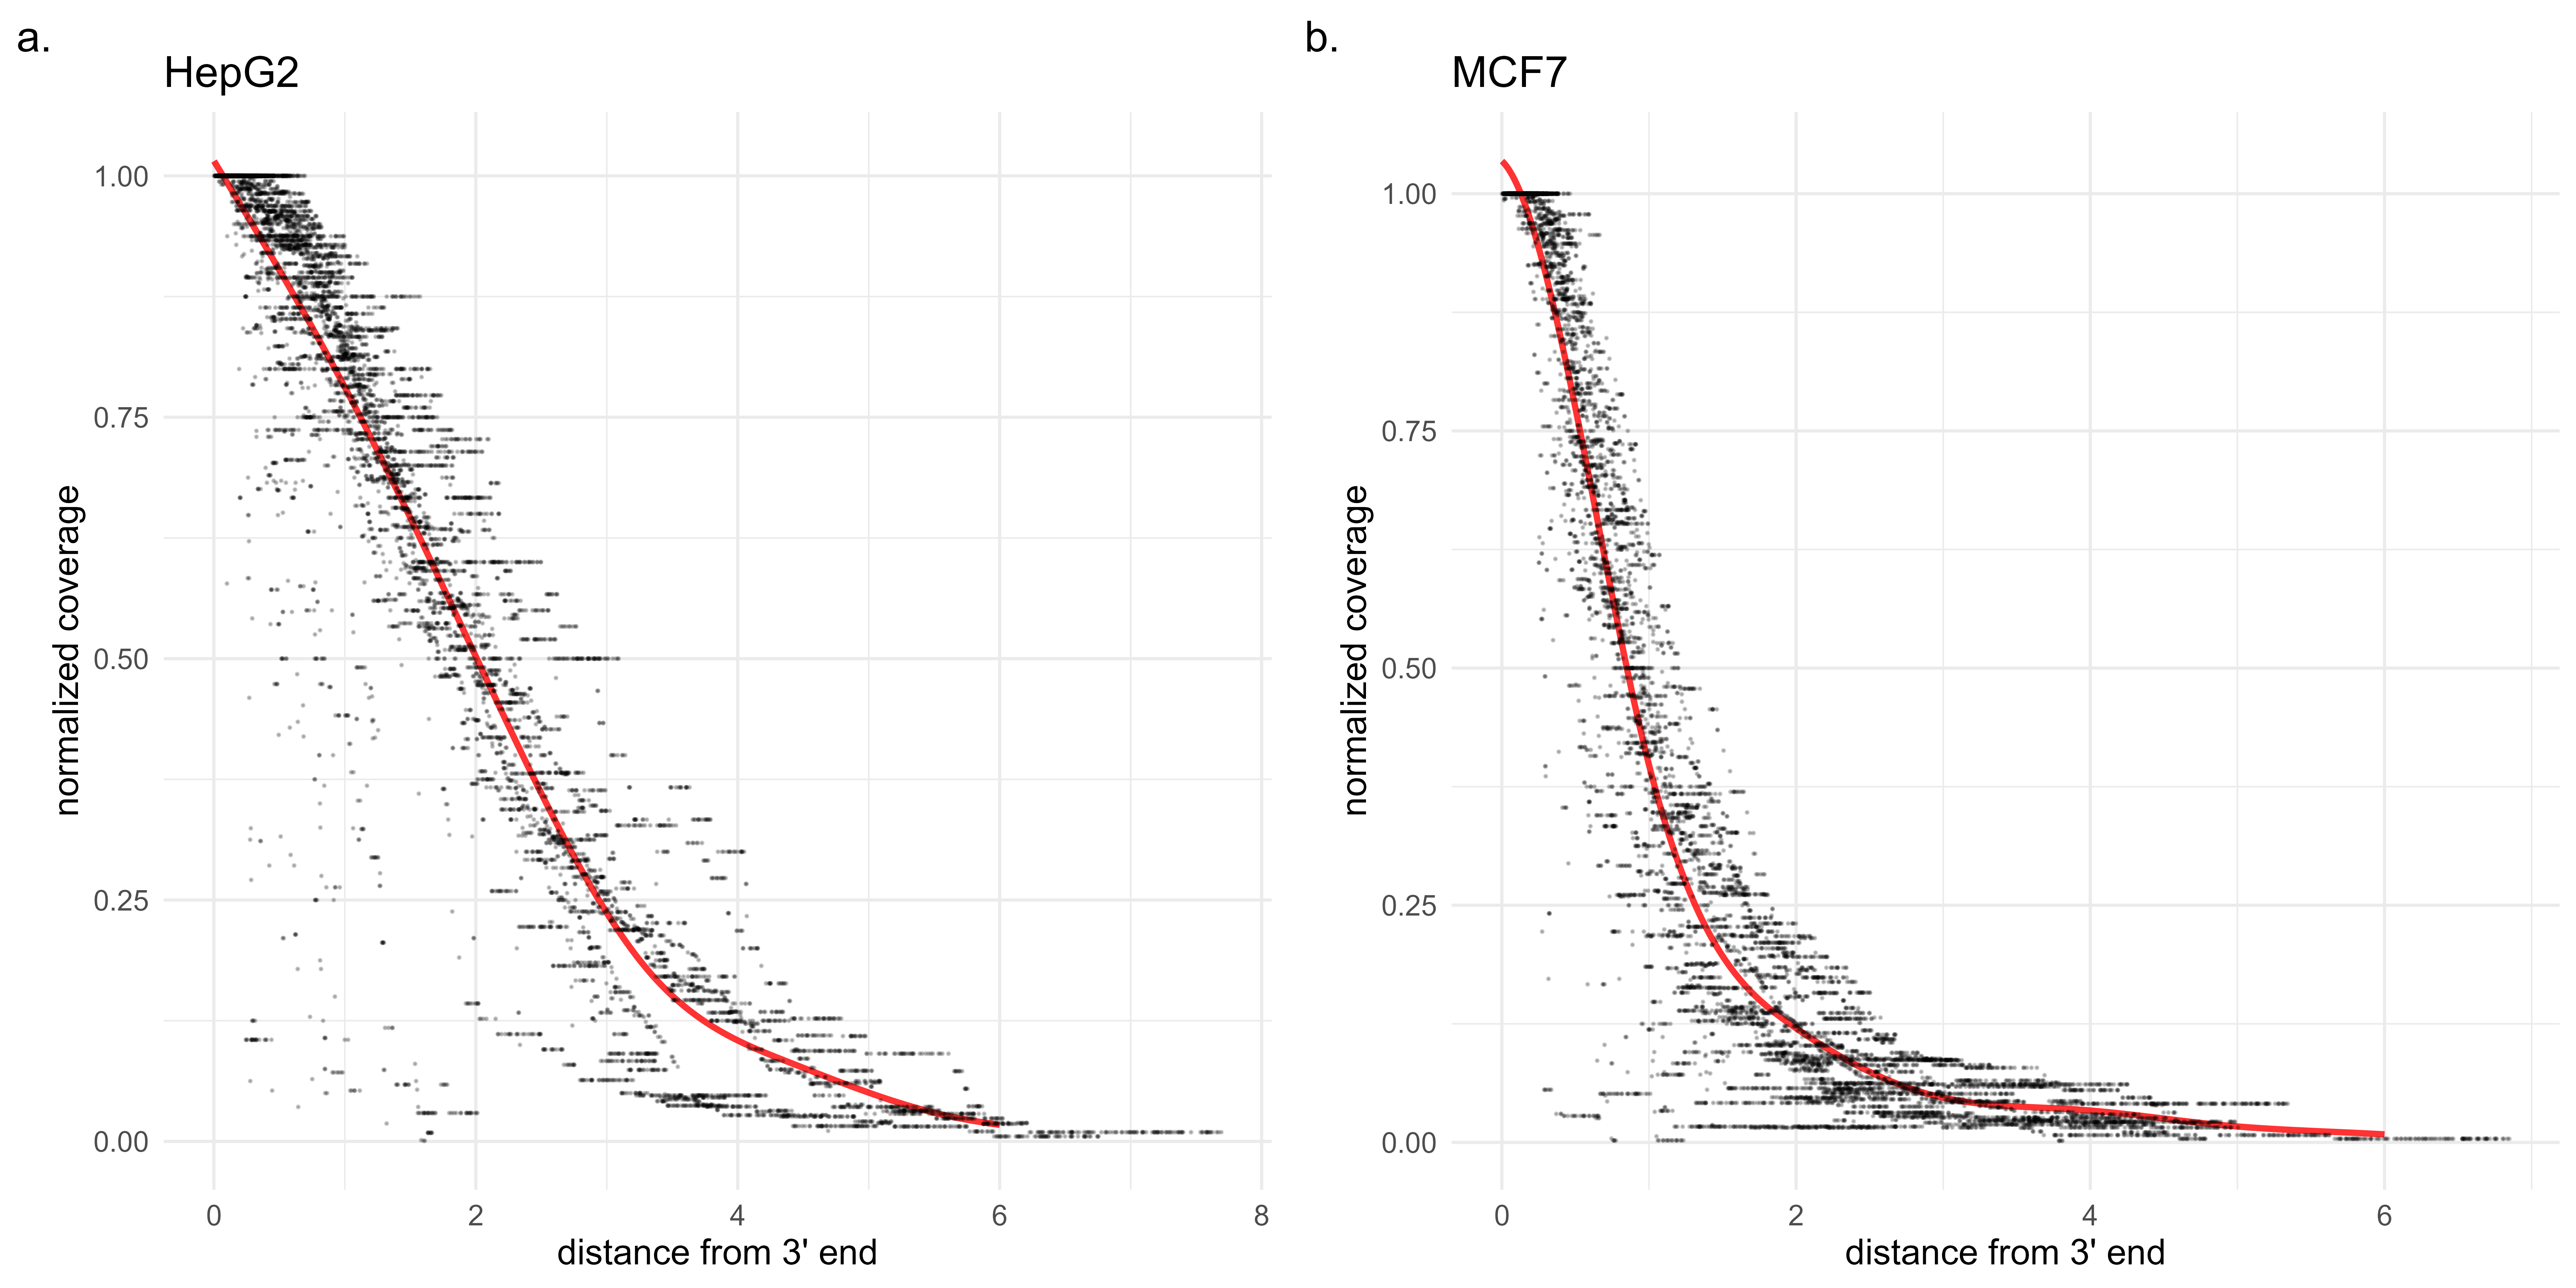
\includegraphics[width=0.9\textwidth]{figures/sec-2-cov-real.png}
    \caption[Degradation curves on real datasets based on coverage]{Degradation curves on real datasets based on coverage. These two datasets has the most isoforms post-filtering for degradation rate estimation. \textbf{a.} Degradation curve for a HepG2 cell line sample. \textbf{b.} Degradation curve for a MCF7 cell line sample.}
    \label{fig:cov-real}
\end{figure}

\subsection{Degradation by isoform features}

Here, we explore whether degradation rates vary between isoforms of different features. In particular, We striate isoforms by their annotated length , observed median coverage (Fig. \ref{fig:cov-feature}b) and biotype (Fig. \ref{fig:cov-feature}c). On a representative sample from the MCF7 cell line, estimated degradation rates do not appear to vary significantly between isoforms of different annotated length or median coverage (Fig. \ref{fig:cov-feature}a,b). However, the converse is true for different transcript biotypes. In particular, we observe higher degradation rates for processed pseudogenes (n = 7) and long non-coding RNAs (n = 3) as compared to protein coding genes (n = 42, Fig. \ref{fig:cov-feature}c). While the sample size here is small, this result corroborates findings in \cite{Clark2012} and \cite{Kaiwan2021}, which identified larger variance in the stabilities of lncRNAs.   

\begin{figure}[H]
    \centering
    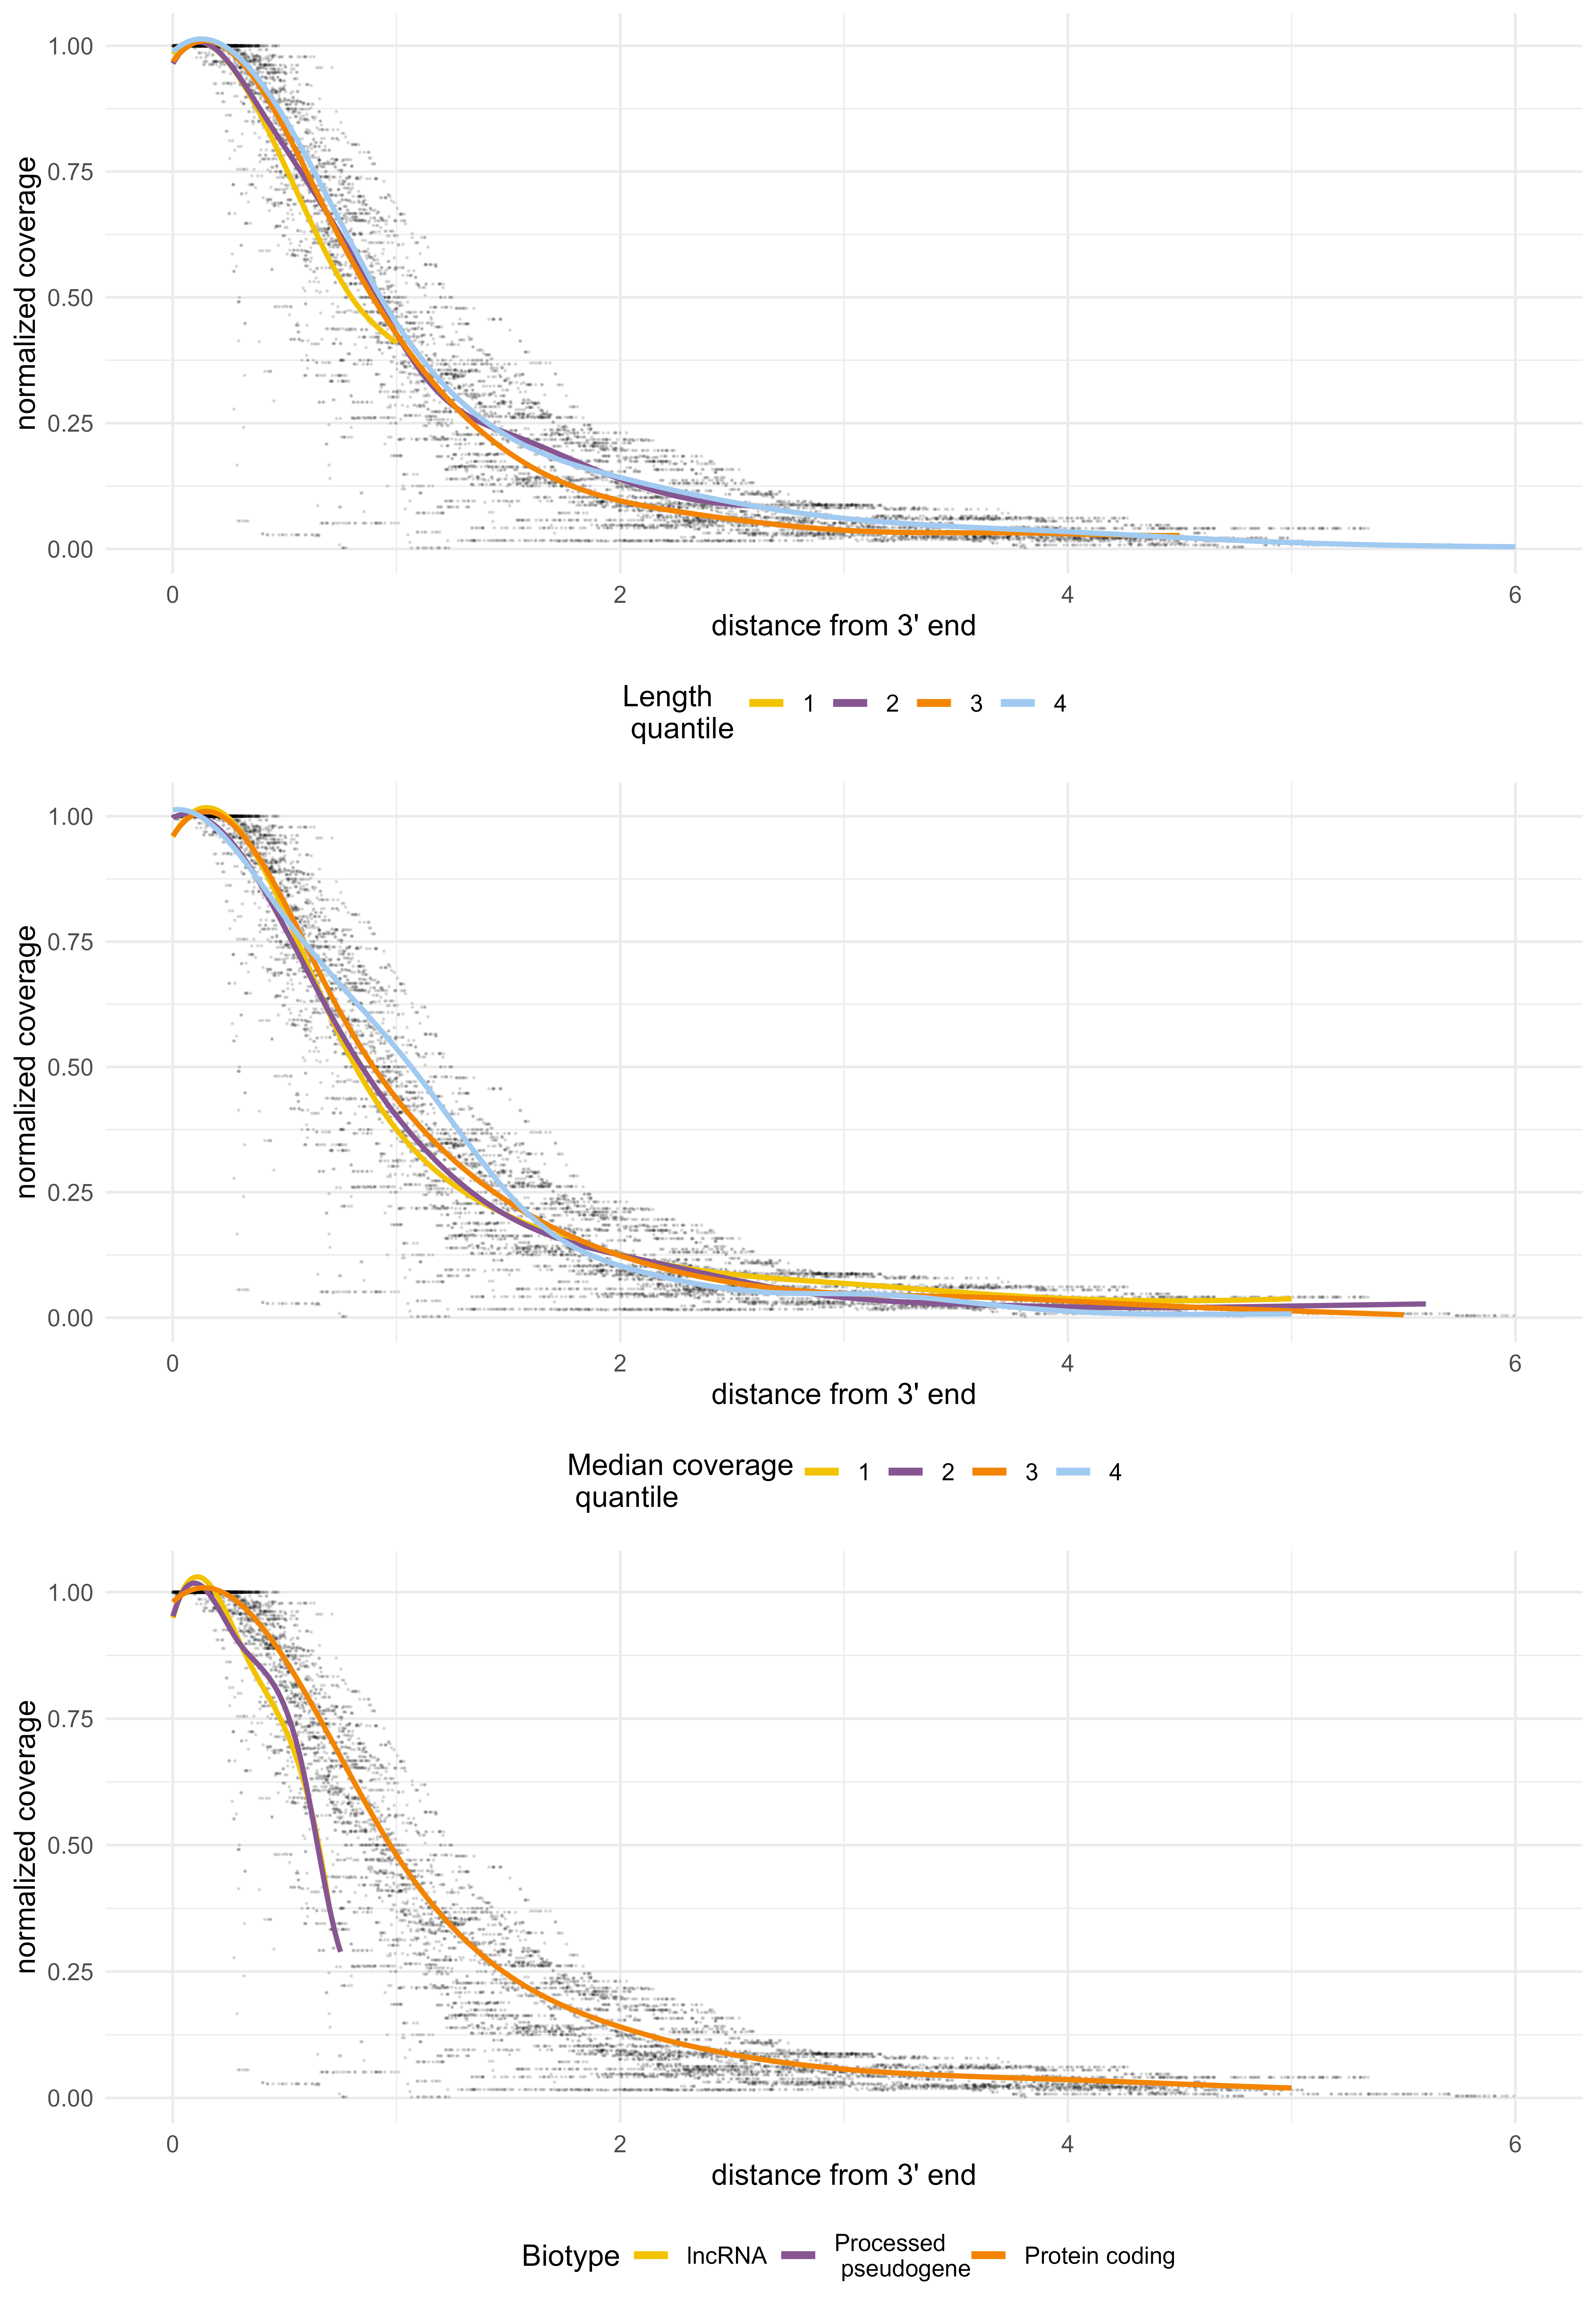
\includegraphics[width=0.95\textwidth]{figures/sec-2-by-feature.png}
    \caption[Degradation curves in MCF7 striated by features]{Degradation curves in MCF7 striated by features. \textbf{a.} Degradation curves fit for isoforms within each length quantile separately, with quantiles at 0\%: 320, 25\%: 1360, 50\%: 2820, 75\%: 5590, 100\%: 9038. \textbf{b.} Degradation curves fit for isoforms within each median coverage quantile separately, with quantiles at 0\%: 7, 25\%: 12, 50\%: 18, 75\%: 31, 100\%: 381. \textbf{c.} Degradation curves fit for isoforms of different biotypes.}
    \label{fig:cov-feature}
\end{figure}

\subsection{Degradation in spike-ins}

We now analyse possible degradation in sequencing spike-ins, which are synthetic RNA molecules added to endogenous RNA samples before library preparation \cite{Lexogen20201}. By doing so, we attempt to elucidate the relative contributions of \textit{in vivo} RNA decay and other extraneous factors unrelated to decay, such as library preparation or sequencing artifacts.

We examine SIRVs (Spike-in RNA Variants) present in a subset of SG-NEx samples. Fortunately, a subset of SIRV isoforms are non-overlapping, allowing us to easily apply coverage-based approaches for estimating the degradation. The degradation curves estimated on the SIRVs for six H9 samples (2 runs with 3 replicates each) show consistent patterns amongst themselves (dotted lines, Fig. \ref{fig:cov-spike}), suggesting a constant extraneous factor that acts on degrading SIRV reads. This is supported by the fact that, within each run, the SIRV degradation rates exhibit strong consistency.

\begin{figure}[H]
    \centering
    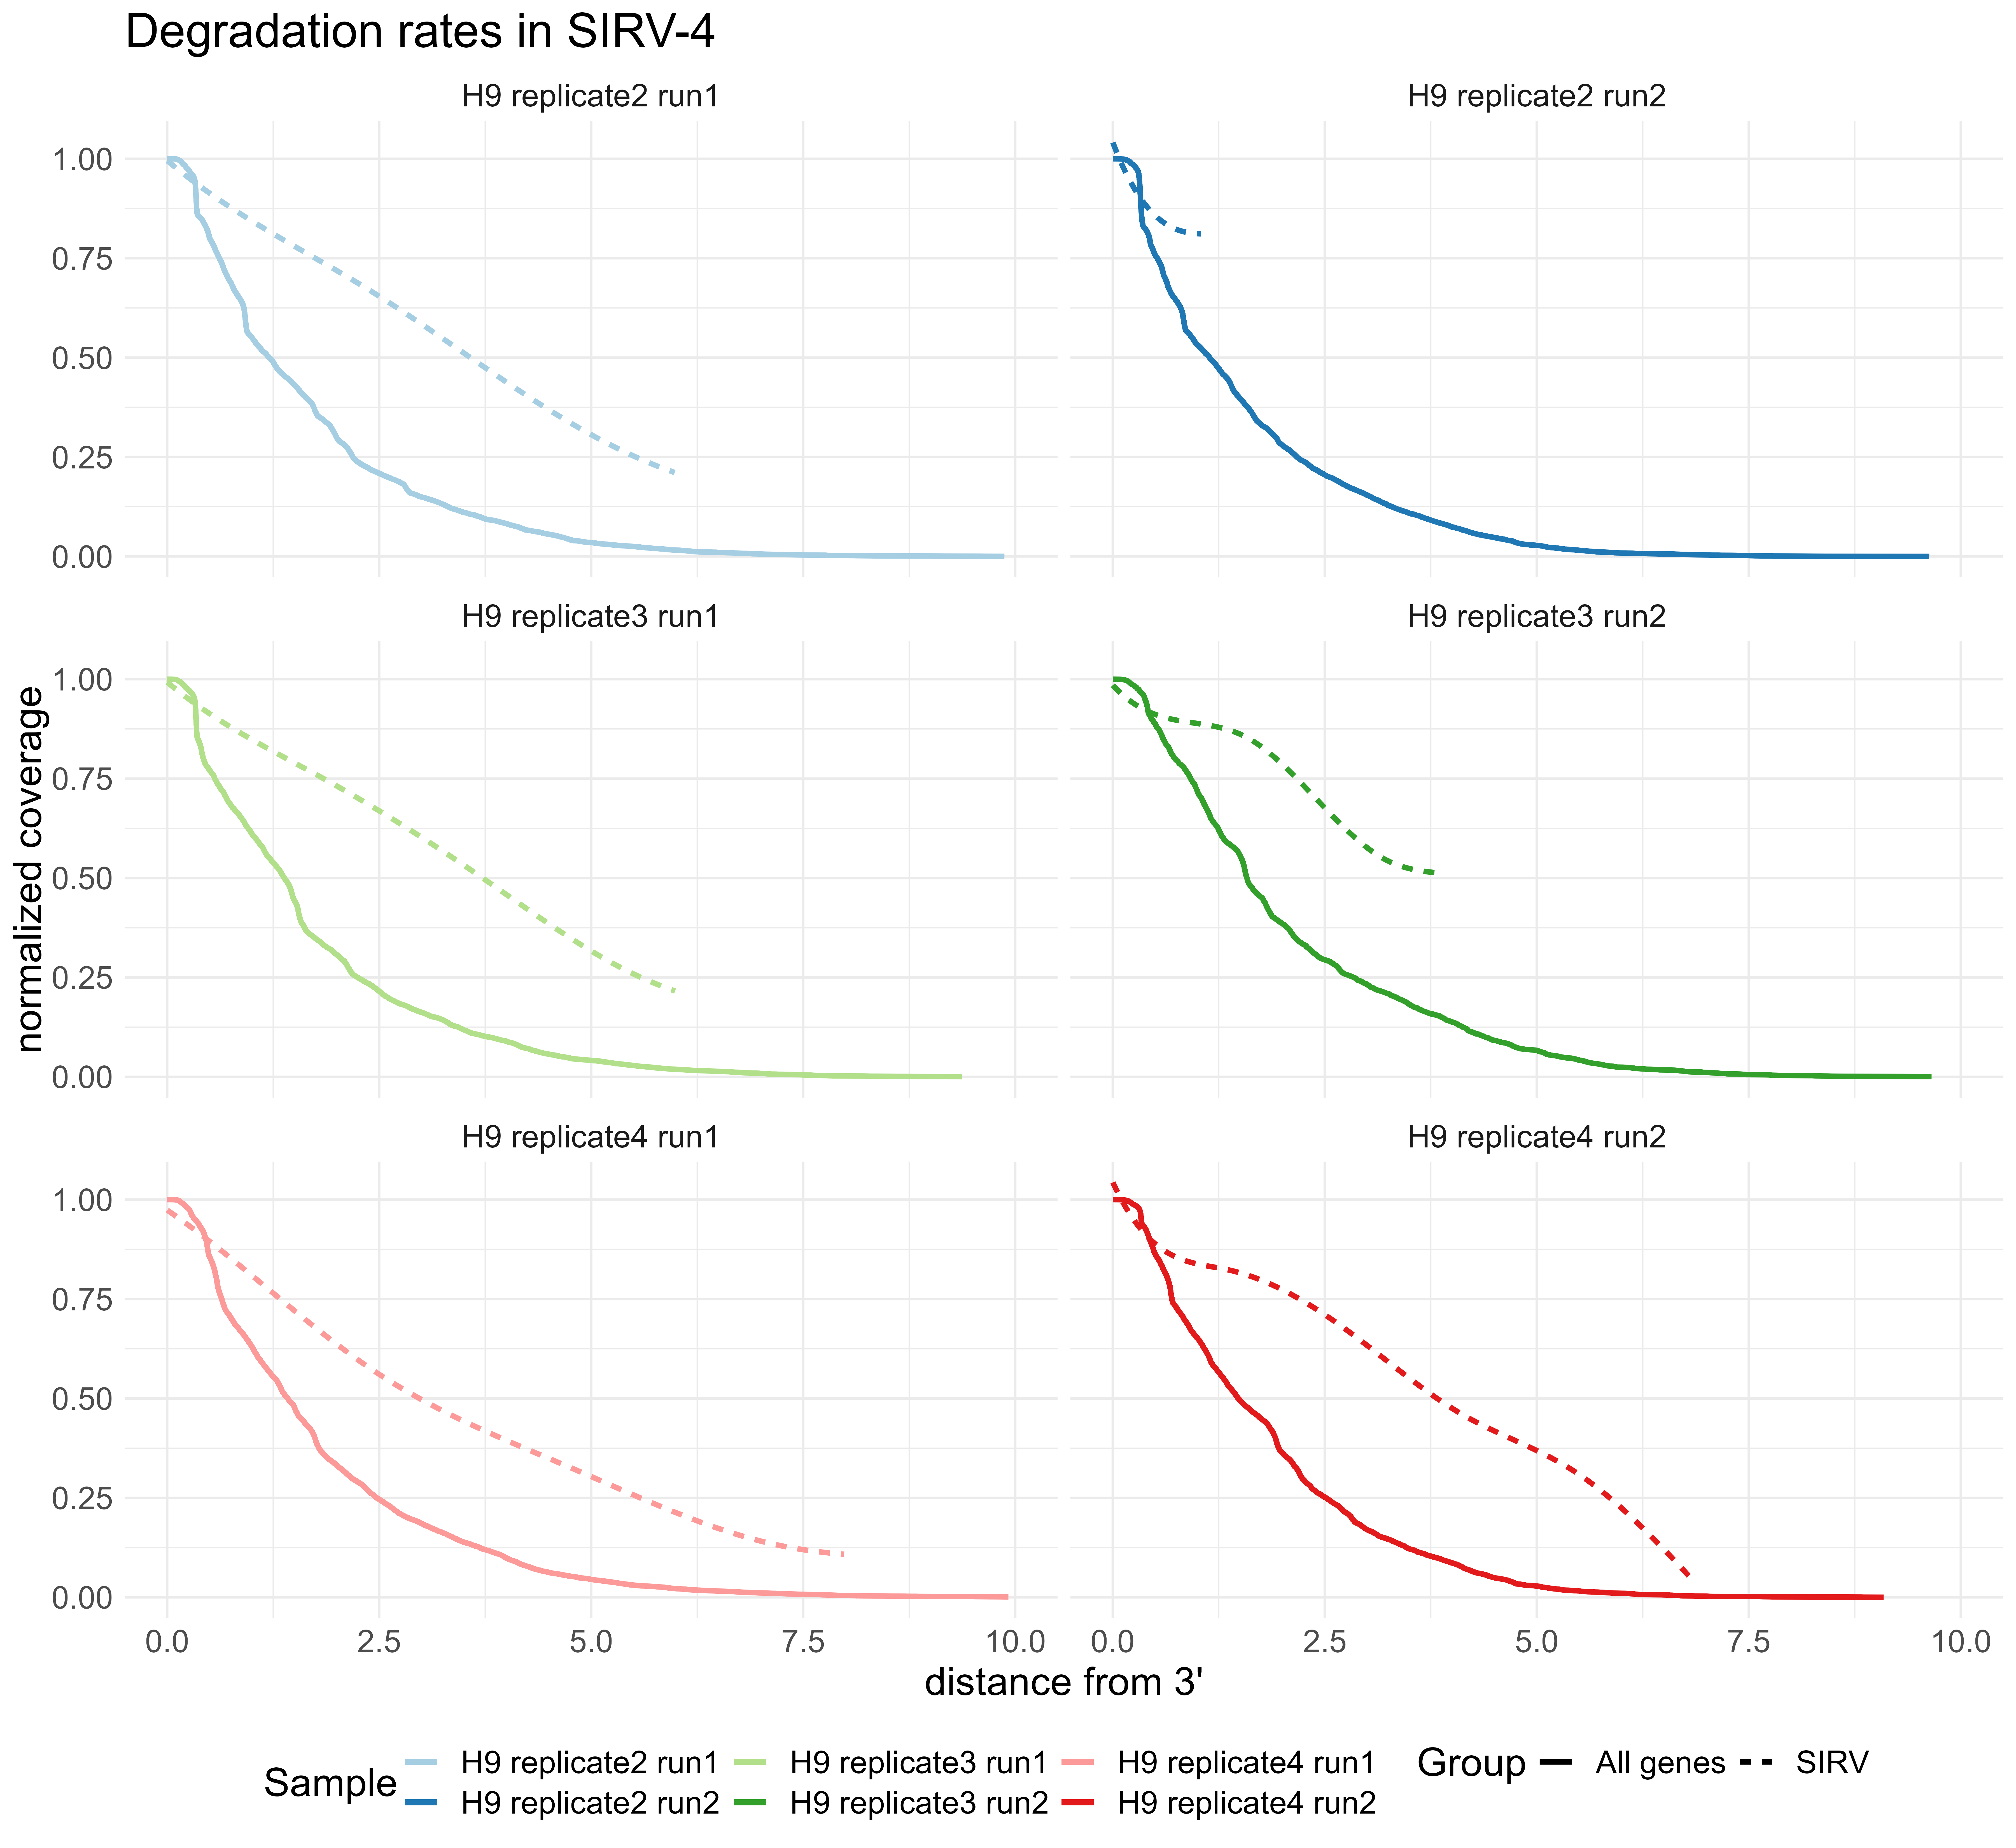
\includegraphics[width=0.9\textwidth]{figures/sec-2-cov-spike.png}
    \caption[Degradation curves for SIRVs based on coverage]{Degradation curves for SIRVs based on coverage for six H9 samples. The number of SIRV transcripts used to fit the degradation curve differs between samples, resulting in curves of different lengths.}
    \label{fig:cov-spike}
\end{figure}

However, when contrasted against degradation curves estimated on all isoforms from within the same sample (solid lines, Fig. \ref{fig:cov-spike}), the SIRVs show lower rates of degradation. This might suggest that the degradation in endogenous RNAs is a combination of RNA decay \textit{in vivo} and extraneous factors. 

\section{Read length-based degradation estimation}\label{sec:rld}

From the coverage-based estimation of degradation in the preceding sections, we gleaned that patterns of degradation tend to be consistent across transcript isoforms for a given sample across annotated length and median coverage. This holds at least for protein coding isoforms. Based on these observations, we develop a more efficient approach for estimating the degradation rate via the observed read length distributions.

Recall that our objective is to estimate the degradation curve, from which we can easily derive the degradation rate. The key observation for developing a read length-based degradation estimation approach is to note that the degradation curve is essentially the survival function on degraded read lengths. Let $X$ be a random variable denoting the length of a read. Then, its survival function is given by 
\begin{equation}
    S(x)=P(X>x)=1-F(x)
\end{equation}
where $F$ is the cumulative distribution function of $X$. Intuitively, the survival function gives the proportion of reads that exceed (survive after) a given length $x$. We make this clear with an illustration on a hypothetical dataset with a degradation rate of 0.2 (Fig. \ref{fig:survival}). Here, the degradation curve provides an easy way to read off the proportion of degraded reads that are at least 1 kb in length, which is $S(1)=0.8$.   

\begin{figure}[H]
    \centering
    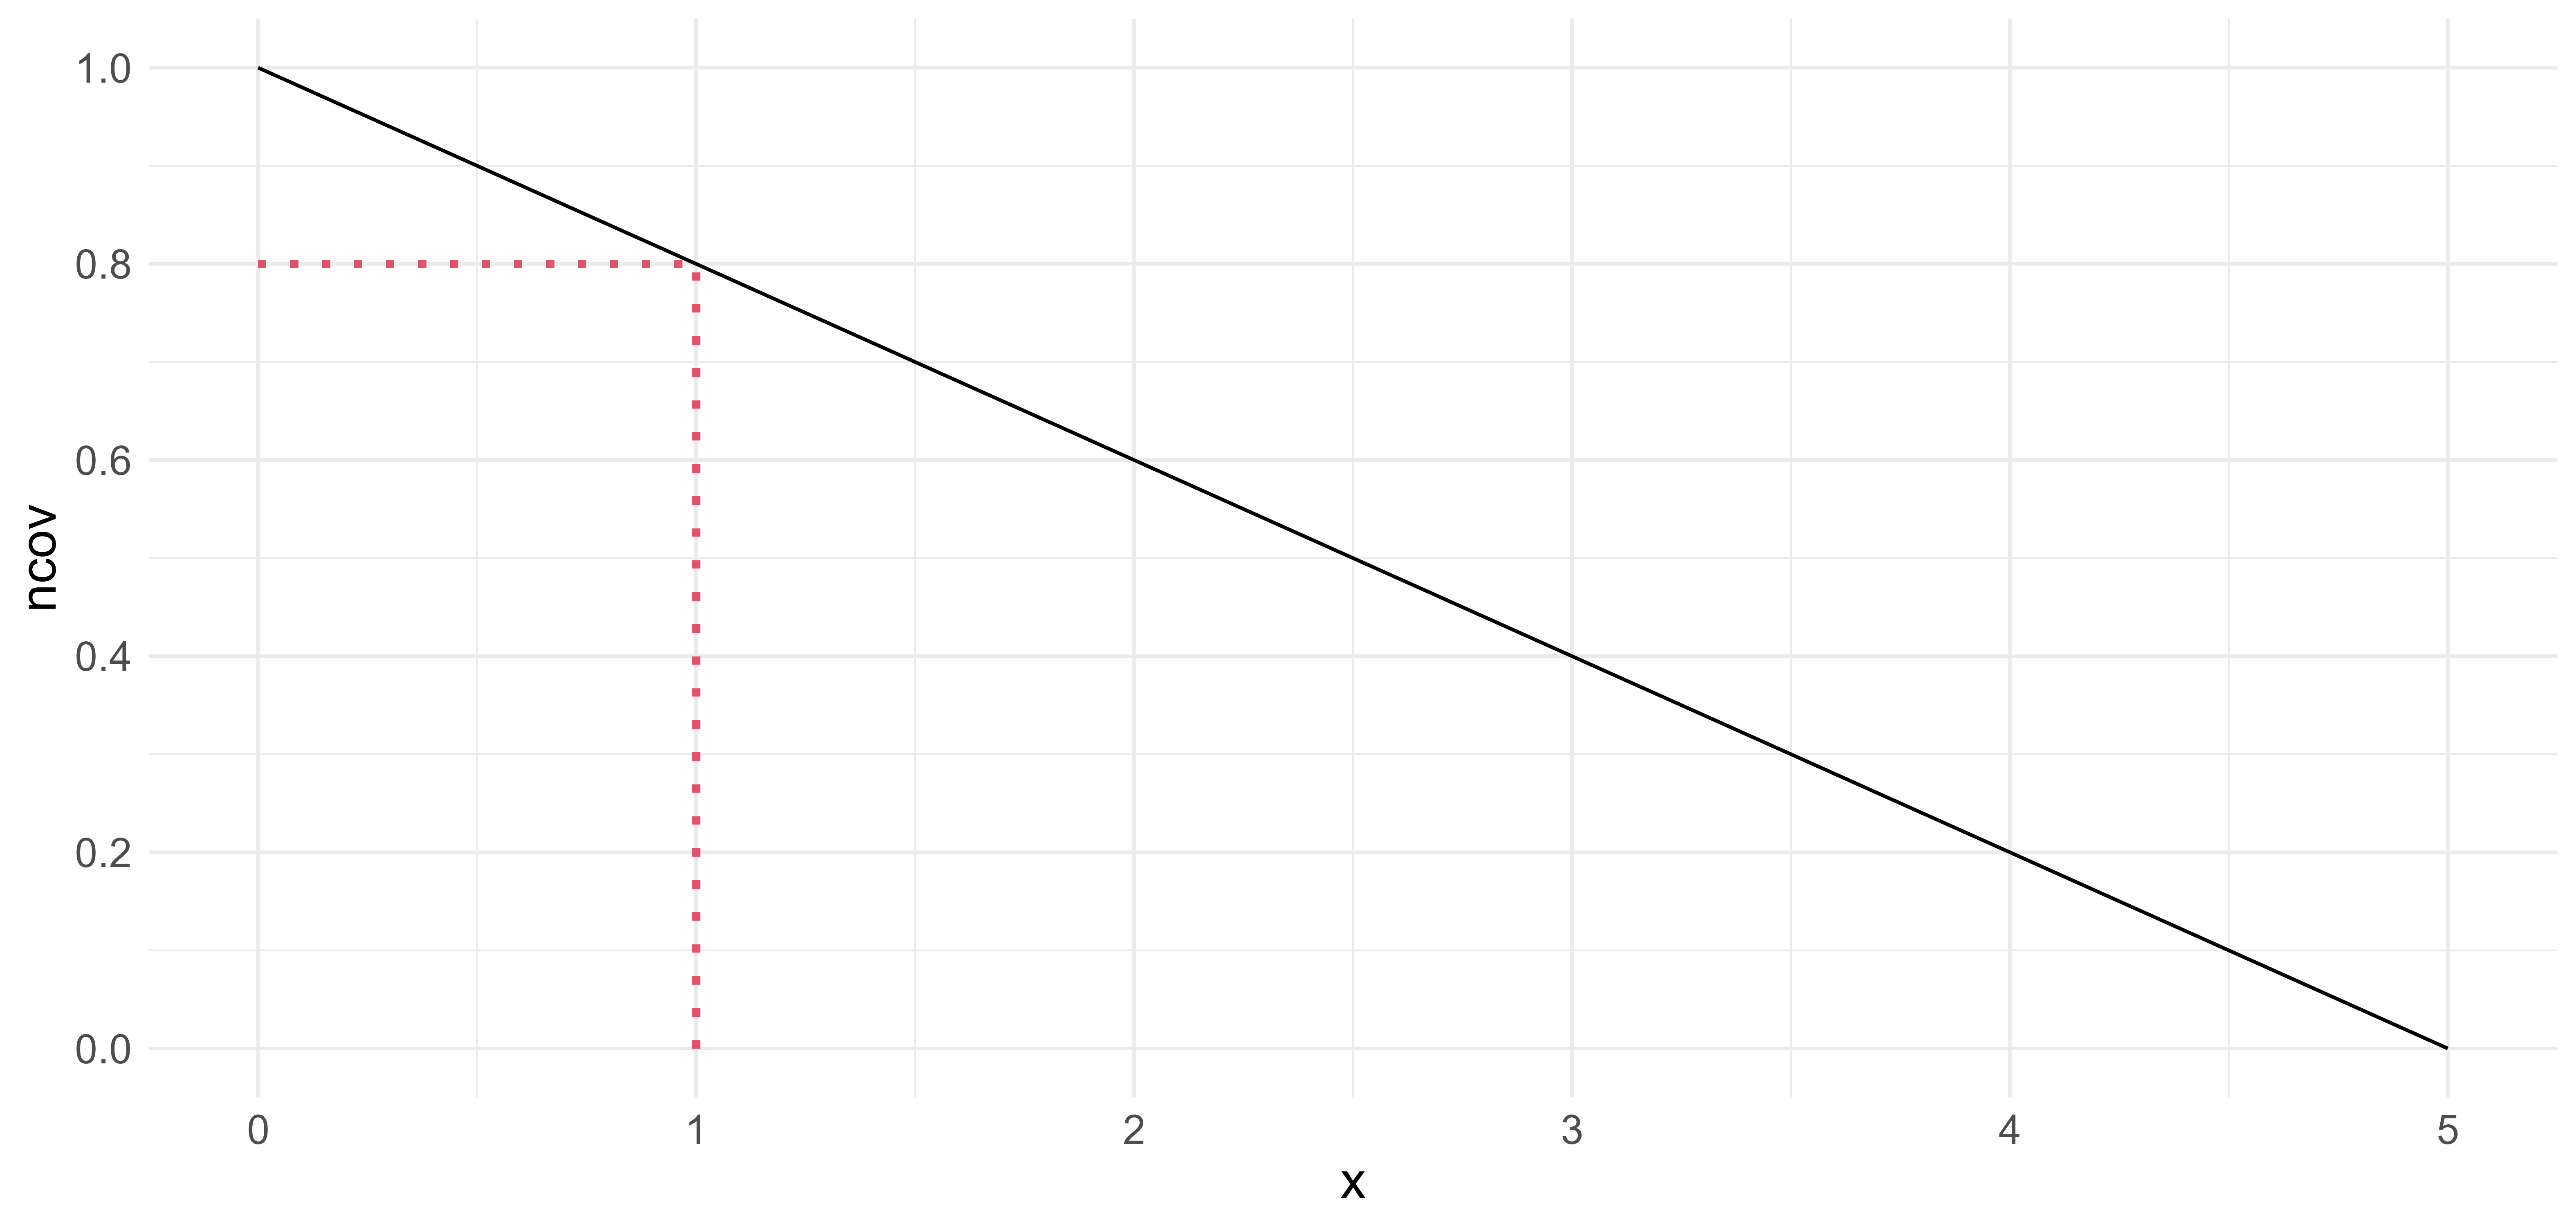
\includegraphics[width=0.85\textwidth]{figures/sec-2-length-example.png}
    \caption[Equivalence between degradation curves and survival functions]{Equivalence between degradation curves and survival functions on degraded read lengths.}
    \label{fig:survival}
\end{figure}

Based on this observation, we develop an approach for estimating degradation based on read length distributions:
\begin{enumerate}
    \item Bin lone isoforms by their length and sample a fixed number of isoforms from each bin. We do so to avoid capturing the isoform length distribution in the degraded read length distribution.  
    \item Extract degraded reads based on the isoforms sampled in step 1. We define degraded reads as those whose lengths are not within the annotated full length by some threshold (in practice, we use 50 bp). 
    \item Compute the empirical cumulative distribution function $F$ on the read lengths obtained in step 2. From here, the degradation curve can be easily computed with $1-F$. 
\end{enumerate}

\begin{figure}[H]
    \centering
    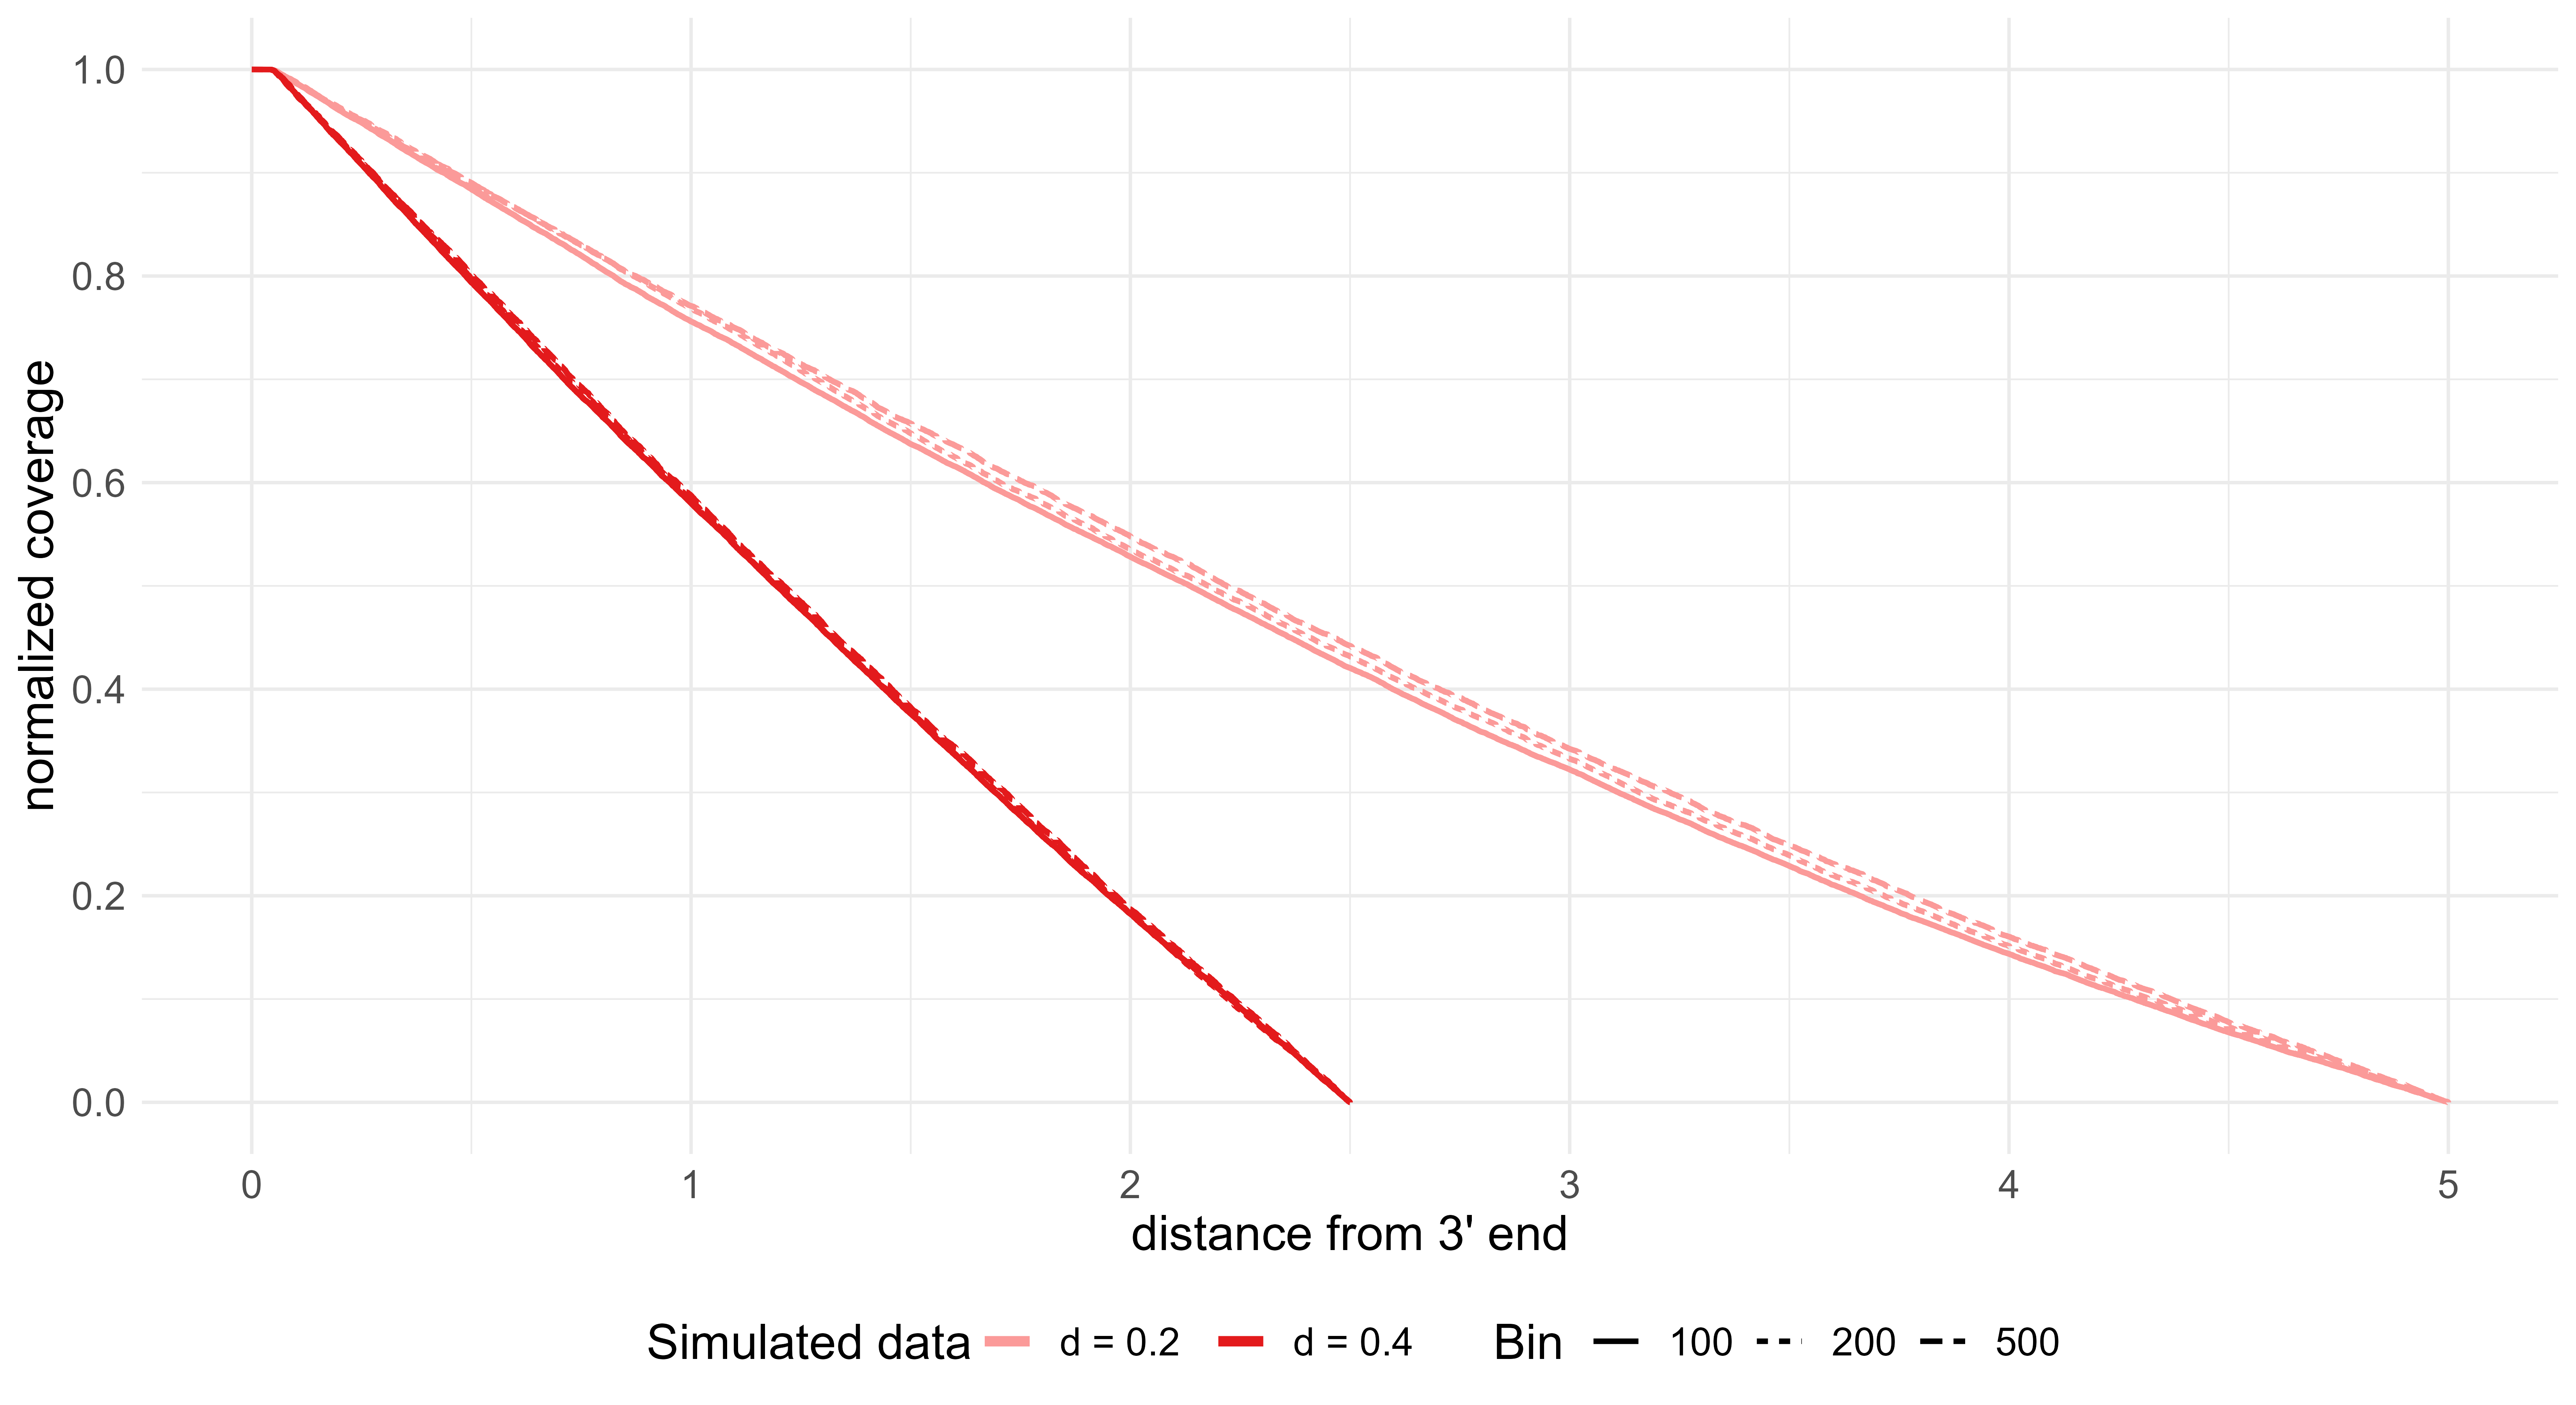
\includegraphics[width=0.85\textwidth]{figures/sec-2-length-sim.png}
    \caption[Degradation curves on simulated datasets based on read length distribution]{Degradation curves on simulated datasets based on read length distribution. For degradation rate of 0.2, coverage drops to 0 at 5 kb (light red), while for degradation rate of 0.4, coverage drops to 0 at 2.5 kb (dark red). The degradation rates are relatively robust to bin size.}
    \label{fig:length-sim}
\end{figure}

\begin{table}[H]
  \centering
    \begin{tabular}{|p{3.5cm}|p{1.5cm}|p{1.5cm}|p{1.5cm}|}
\cline{2-4}    \multicolumn{1}{r|}{} & \multicolumn{3}{c|}{Bin size} \bigstrut\\
    \hline
    Simulated dataset & 100   & 200   & 500 \bigstrut\\
    \hline
    d = 0.1 & 0.118 & 0.113 & \textbf{0.107} \bigstrut\\
    \hline
    d = 0.2 & 0.207 & 0.206 & \textbf{0.204} \bigstrut\\
    \hline
    d = 0.4 & \textbf{0.408} & 0.409 & \textbf{0.408} \bigstrut\\
    \hline
    d = 0.5 & 0.513 & 0.512 & \textbf{0.511} \bigstrut\\
    \hline
    \end{tabular}%
  \caption[Degradation estimates on simulated datasets based on read length distribution]{Degradation estimates on simulated datasets based on read length distribution. The length bin size is varied for 100, 200 and 500 bp, and the average degradation rate is computed.}
  \label{tab:binsize}%
\end{table}%

We validate this approach on the same simulated datasets with degradation rate of 0.2 and 0.4 and test the robustness of the length bin size used. The degradation curves qualitatively reflect the expected degradation rate (Fig. \ref{fig:length-sim}) and appear robust to the bin size chosen (Table \ref{tab:binsize}). We note that in the range of bin sizes we tested, a larger bin size yielded estimates closest to the expected degradation rates. Intuitively, a smaller bin size captures more variance in the degraded read length distribution, making the estimates noisier.         

With this validation in hand, we estimated degradation rates for 32 direct RNA-seq samples spanning six cell lines and six sequencing runs for multiple bin sizes (Table \ref{tab:six-six}). In general, degradation rates within a cell line varied across the samples (Fig. \ref{fig:length-sgnex}a), presumably due to variations in sequencing runs (Fig. \ref{fig:length-sgnex}b).   

\begin{table}[H]
  \centering
    \begin{tabular}{|p{1.5cm}|p{1.5cm}|p{1.5cm}|p{1.5cm}|p{1.5cm}|p{1.5cm}|p{1.5cm}|}
\cline{2-7}    \multicolumn{1}{l|}{} & Run1  & Run2  & Run3  & Run4  & Run5  & Run6 \bigstrut\\
    \hline
    A549  & 4     & 0     & 0     & 0     & 0     & 0 \bigstrut\\
    \hline
    H9    & 4     & 3     & 0     & 0     & 0     & 0 \bigstrut\\
    \hline
    Hct116 & 3     & 1     & 2     & 1     & 1     & 1 \bigstrut\\
    \hline
    HepG2 & 3     & 1     & 1     & 0     & 0     & 0 \bigstrut\\
    \hline
    MCF7  & 2     & 1     & 0     & 0     & 0     & 0 \bigstrut\\
    \hline
    K562  & 4     & 0     & 0     & 0     & 0     & 0 \bigstrut\\
    \hline
    \end{tabular}%
      \caption[Description of SG-NEx samples across cell lines and sequencing runs]{Description of SG-NEx samples across cell lines and sequencing runs}
  \label{tab:six-six}%
\end{table}%

Examining the degradation curves for all samples within sequencing run 1, we observe that 



\begin{figure}[H]
    \centering
    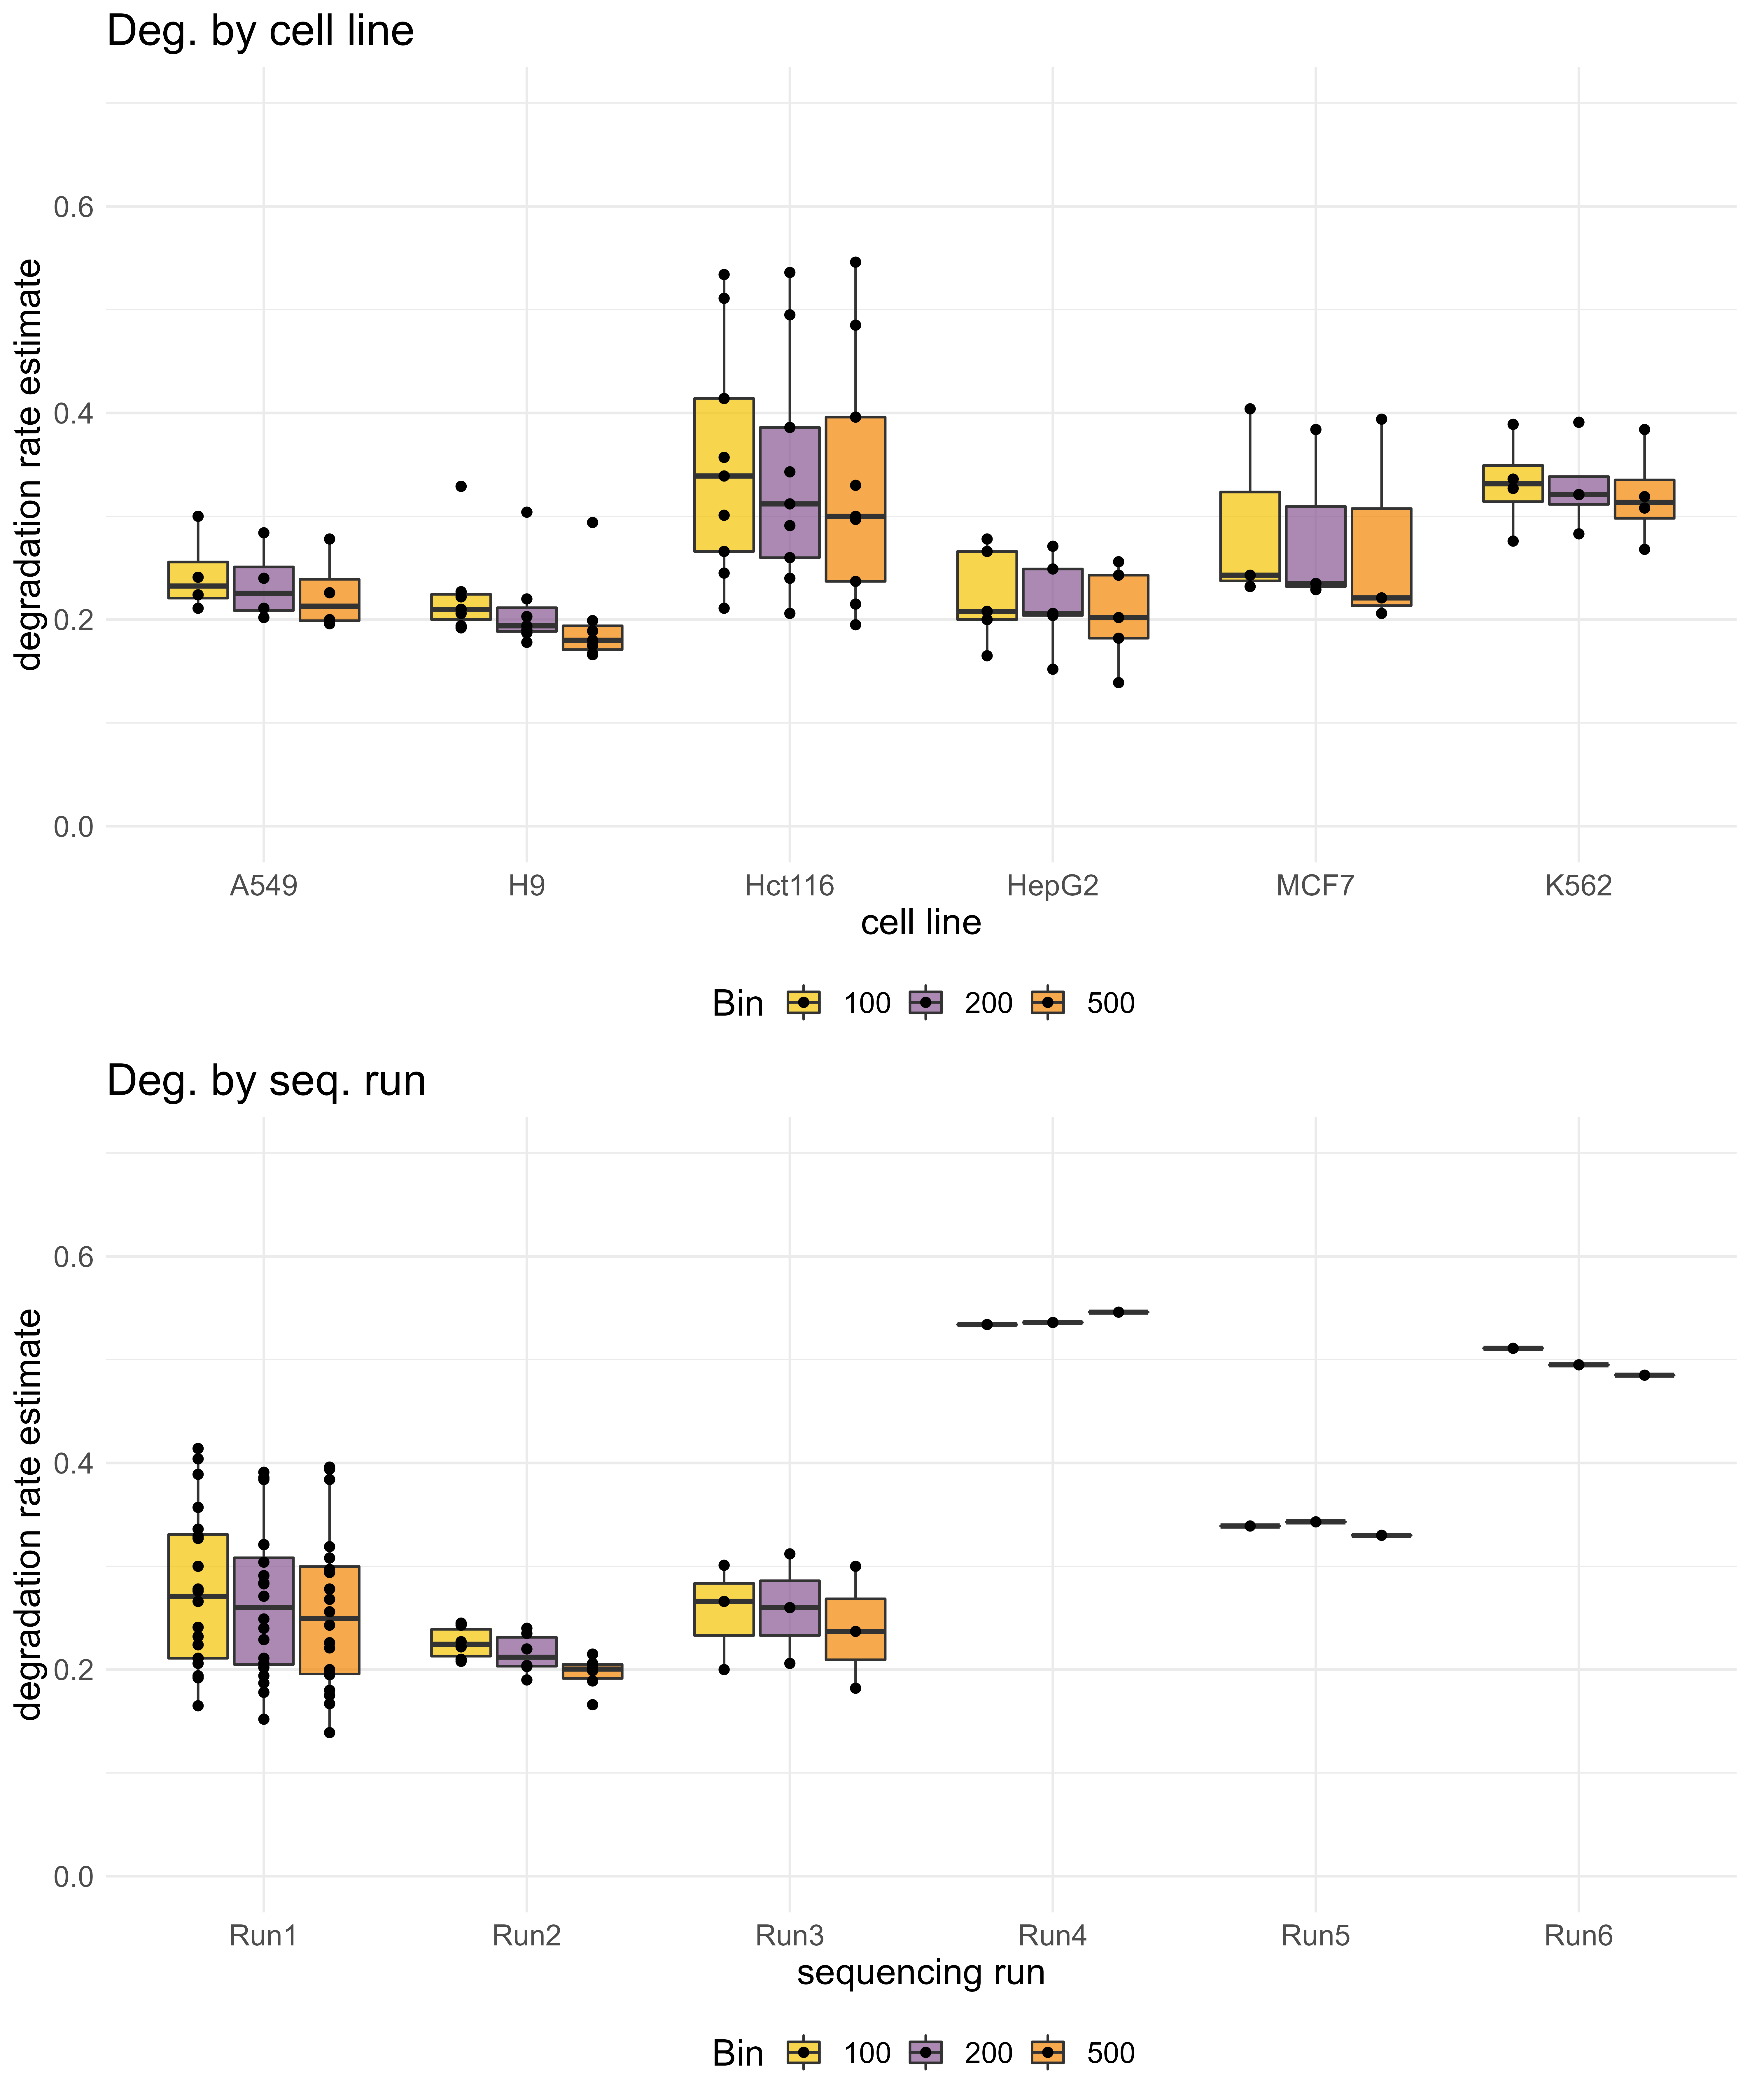
\includegraphics[width=\textwidth]{figures/sec-2-length-sgnex.png}
    \caption[Degradation estimates for real datasets based on read length distribution]{Degradation estimates for real datasets based on read length distribution. \textbf{a.} Samples grouped by cell line. \textbf{b.} Samples grouped by sequencing run.}
    \label{fig:length-sgnex}
\end{figure}

\begin{figure}[H]
    \centering
    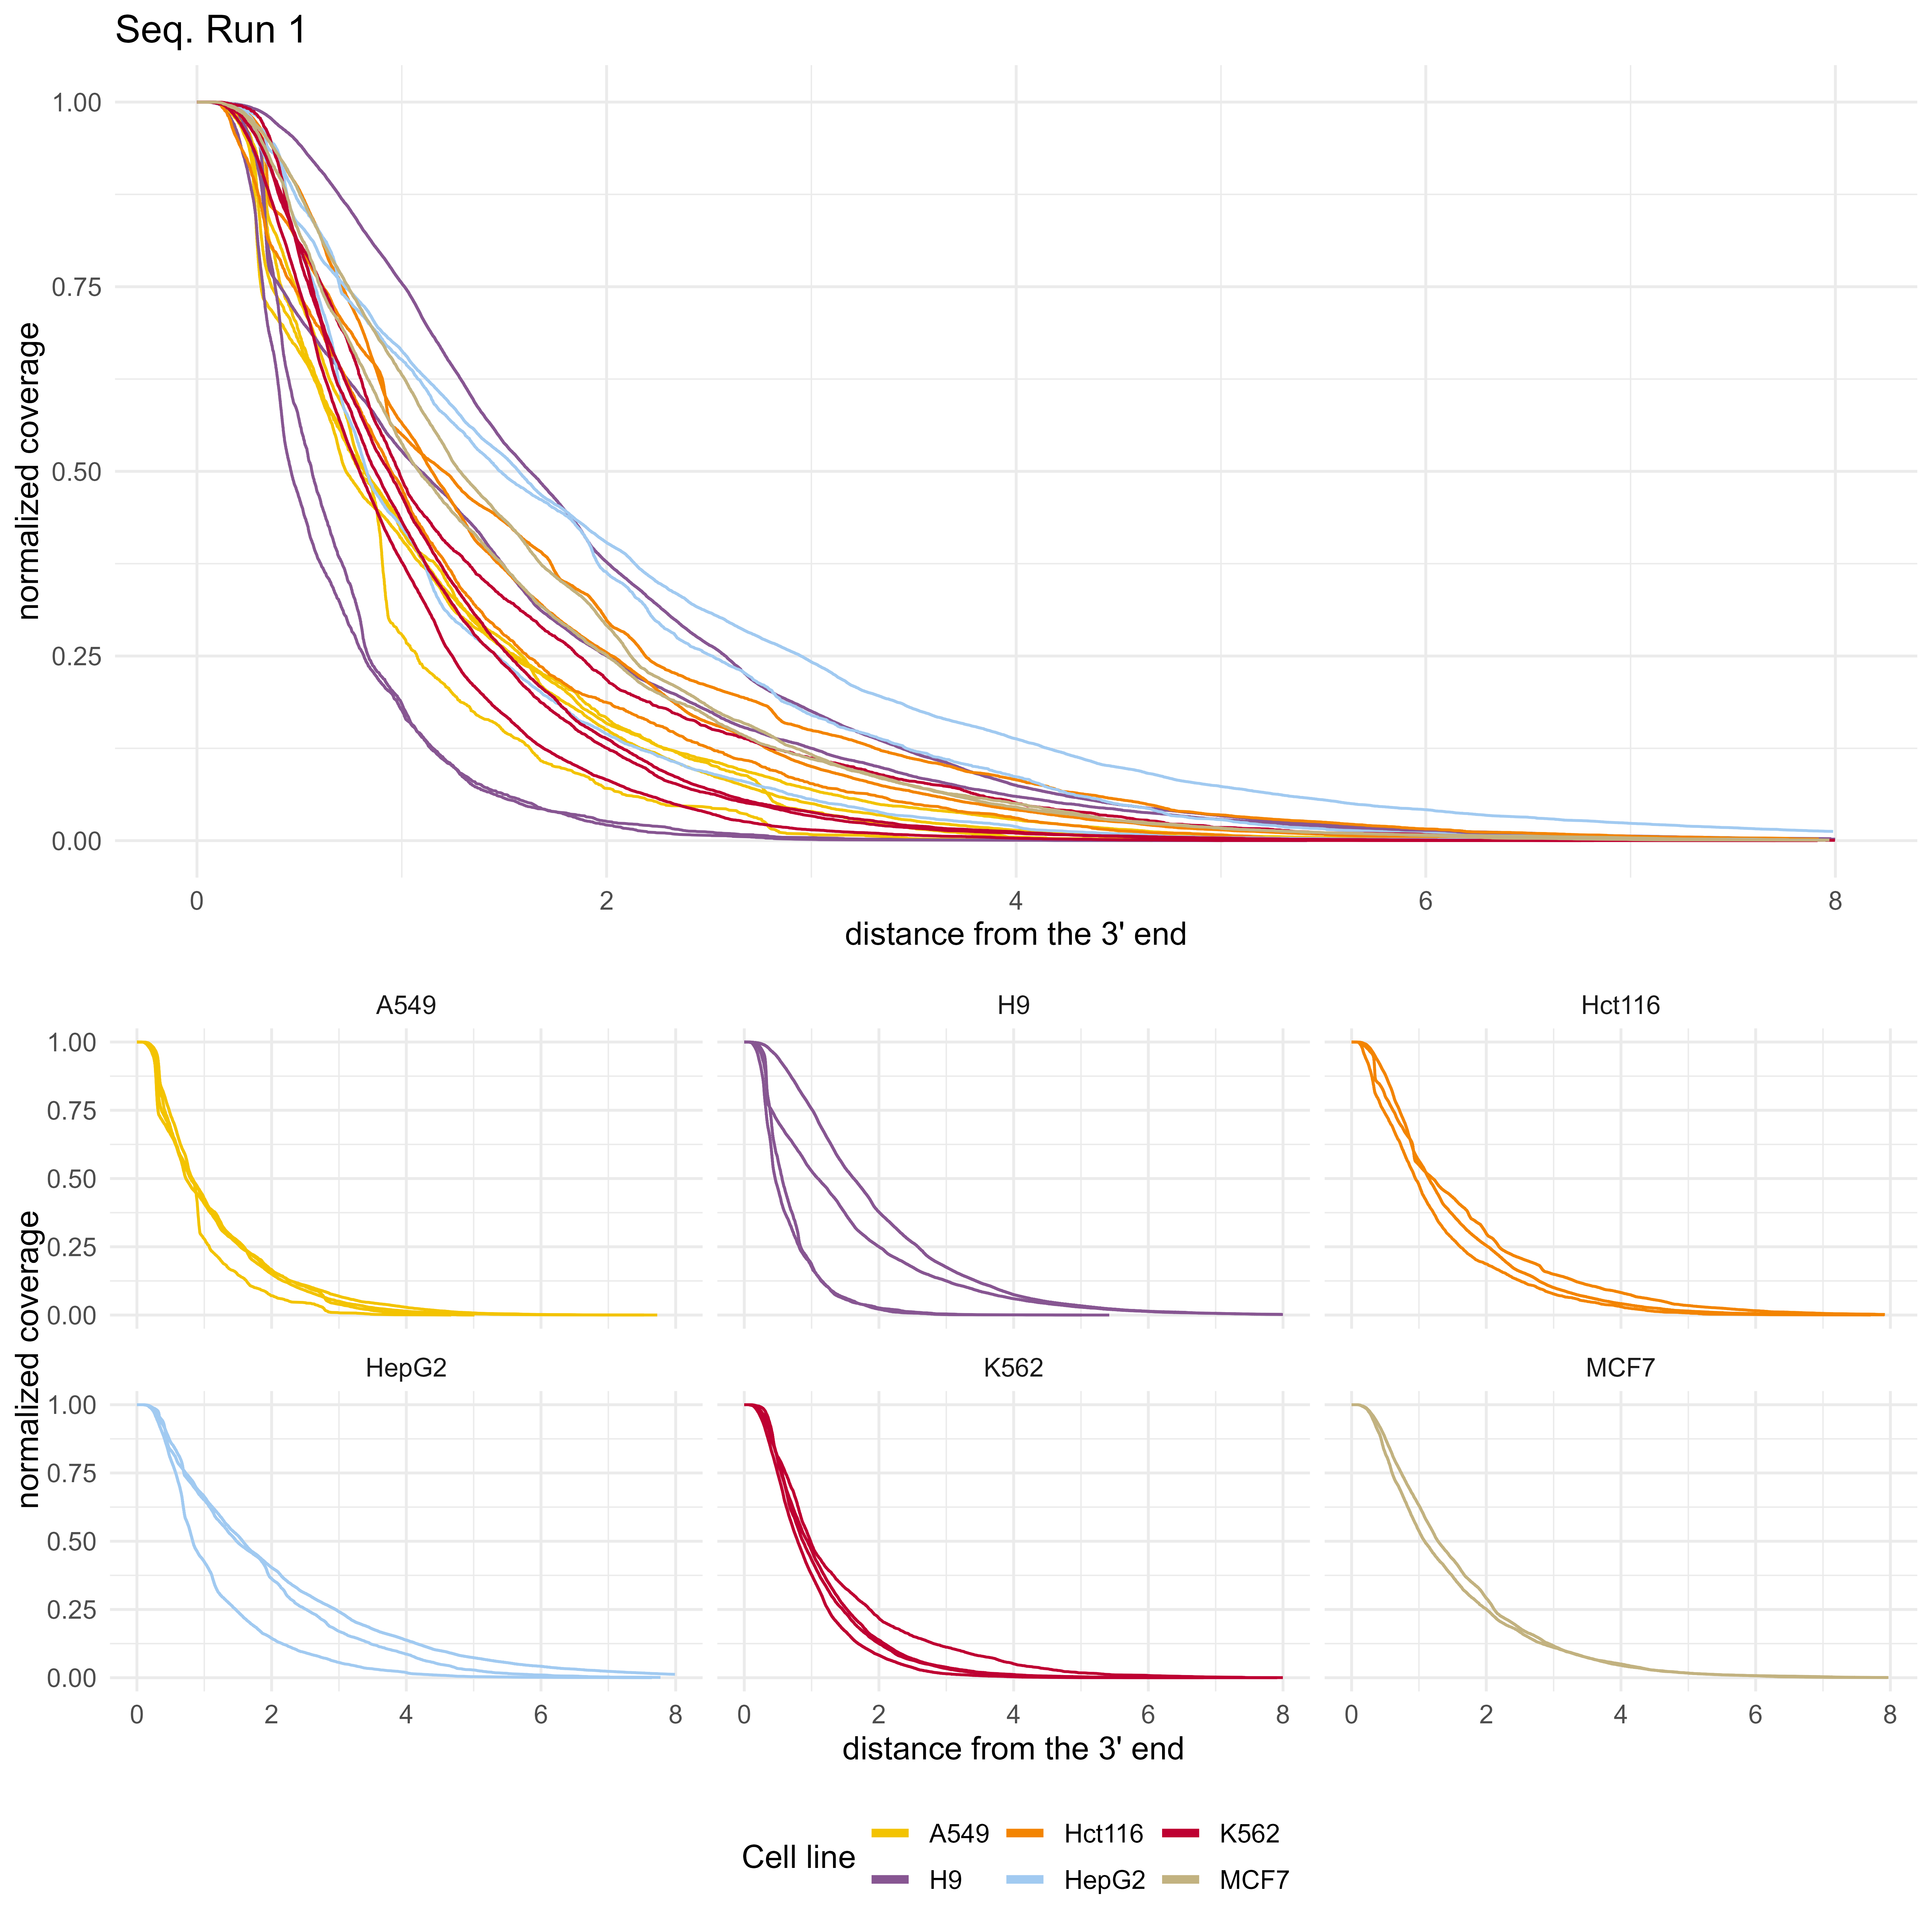
\includegraphics[width=\textwidth]{figures/sec-2-length-sgnex-curves.png}
    \caption[Degradation curves for real datasets based on read length distribution]{Degradation curves for real datasets based on read length distribution for sequencing run 1. The top panel shows all samples combined. The bottom panel splits the samples by cell lines.}
    \label{fig:length-sgnex}
\end{figure}



\chapter{Bias-aware quantification}

In this chapter, we specify a generative model for transcript quantification from long-read direct \gls{rnaseq} that accounts for bias due to degradation of \gls{mrna} transcripts. We detail the assumptions of our model, formulate the generative process and derive statistical algorithms for inference of the parameters of the model.  

\section{Model assumptions}\label{sec:model-assumptions}

The input to our model consists of reads obtained from sequencing transcripts with the \gls{ont} direct \gls{rnaseq} protocol aligned to the reference transcriptome. We assume there is a bijective mapping between reads and transcript, i.e., each read originates from only one transcript, and each transcript generates only one read. Reads are generated independently and identically distributed (iid) from a distribution to be specified, and the 3' end of each read aligns within some region close to the 3' end of the isoform it originated from.

We make two assumptions on the degradation rate $d$. First, we assume that the degradation of a transcript does not depend on the expression level or biotype of the isoform it originated from. Second, we assume that the expected degradation rate is constant, i.e, $\mathbb{E}[d]=c\in(0,1)$. Even though the second assumption is relatively strong (see Section \ref{sec:read-length-isoform-agreement}), we make this simplifying assumption to show that our model works on simulated data, and relax this assumption to allow our model to generalize to real datasets. 

\section{Generative model}\label{sec:generative-model}

Our model aims to capture the generative process of the observed degraded reads from their isoforms of origin. Here, we formalize our model and derive the complete data log likelihood for maximum likelihood estimation of the model parameters. 

\subsection{Notation and formulation}\label{sec:notation-and-formulation}

Let $N$ be the number of observed reads and $M$ be the number of isoforms the reads were generated from. 
\begin{itemize}
    \item We observe a set of reads $\bm{R}=\{r_1,...,r_N\}$, with $r_i$ representing the $i$\ts{th} read. The variable $r_i$ can be thought of as a collection of properties about the $i$\ts{th} read that are relevant for quantification, such as length, start and end positions or GC content.
    \item Our goal is to infer the unknown relative abundances of the isoforms $\bm{\theta}=\{\theta_1,...\theta_M\}$. These relative abundances sum to one and are non-negative, i.e., $\Sigma_j\theta_j=1, \theta_j\geq0$ $\forall j$. 
    \item We introduce $N$ latent variables $\bm{Z}=\{z_1,...,z_N\}$, where $z_i=(z_{i1}$ $...$ $z_{iM})^T$ is a binary vector in $M$-dimensions with $\Sigma_jz_{ij}=1$. $z_i$ describes the assignment of $r_i$ to one of $M$ isoforms, where
    \begin{equation}
        z_{ij} = 
        \begin{cases}
        1 & \text{if } r_i \text{ originated from isoform } j\\
        0 & \text{otherwise }
        \end{cases}
    \end{equation}
\end{itemize} 
The directed graphical model in Figure \ref{fig:graphical-model-1} illustrates the relationship between the variables $\bm{R}, \bm{Z}$ and parameters $\bm{\theta}$, and provides an easy way to read off the factorization of the joint distribution over the observed and latent variables:
\begin{equation}
    p(\bm{R},\bm{Z})=p(\bm{R}\mid\bm{Z})\cdot p(\bm{Z})\label{eq:joint-dist}
\end{equation}
\begin{figure}[H]
    \centering
    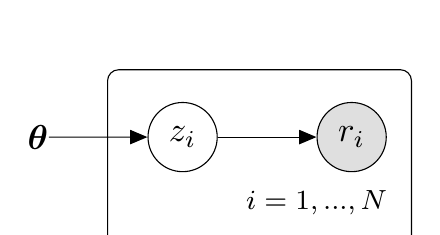
\begin{tikzpicture}[scale=1.25, every node/.style={transform shape}]
        \node[const](theta){$\bm{\theta}$}; % 
        \node[latent, right=of theta](z){$z_i$}; %
        \node[obs, right=of z](r){$r_i$}; %
        \edge{theta}{z}; %
        \edge{z}{r}; %
        \plate[inner sep=0.4cm, xshift = -0.1cm]{plate1}{(z)(r)}{$i=1,...,N$}; %
    \end{tikzpicture}
    \caption[Graphical model for long-read RNA-seq]{Graphical model for long-read RNA-seq. Nodes are random variables, and directed edges represent the dependencies between them. Shaded nodes are observed, while unshaded nodes are latent. Variables within the plate are replicated $N$ times.}
    \label{fig:graphical-model-1}
\end{figure}
\noindent The distribution over the latent variables is categorical:
\begin{equation}
    p(z_i)=\prod_{j=1}^M \theta_j^{z_{ij}}\label{eq:latent-dist}
\end{equation}
The conditional distribution of observing the read $r_i$ given $z_i$ is
\begin{equation}
    p(r_i\mid z_i)=\prod_{j=1}^M p(r_i\mid z_{ij})^{z_{ij}}\label{eq:cond-dist}
\end{equation}
We now model the probability that read $i$ originated from isoform $j$, i.e., $p(r_i\mid z_{ij}=1)$. This probability is proportional to:
\begin{itemize}
    \item The alignment compatibility $a_{ij}\in(0,1)$ between read $i$ and isoform $j$, which measures the alignment score (AS) of read $i$ against isoform $j$ scaled by the best alignment score of read $i$ against all isoforms:
    \begin{equation}
        a_{ij} = \frac{{\textrm{AS}}_{ij}}{\max_{j'} {\textrm{AS}}_{ij'}}
    \end{equation}
    \item The probability of observing a read of length $\ell_i$ given the degradation rate $d_j$ of isoform $j$, i.e., $p(\ell_i\mid d_j, \mathrm{len}(j), z_{ij}=1)$, where $\ell_i$ is the length of $r_i$. We refer to this probability as the \textit{read length-isoform agreement} model.      
\end{itemize}
Combining alignment compatibility and the read length-isoform agreement model, we have 
\begin{equation}
    p(r_i\mid z_{ij}=1) = a_{ij}\cdot p(\ell_i\mid d_j, z_{ij}=1)\label{eq:read-iso-agreement}
\end{equation}
We make some remarks on equation \ref{eq:read-iso-agreement}. First, $a_{ij}$ measures how well read $i$ aligns to isoform $j$ compared to its best alignment. Note that if we do not observe an alignment between read $i$ and isoform $j$, then $\mathrm{AS}_{ij}=0$, $a_{ij}=0$, and thus $p(r_i\mid z_{ij}=1)=0$ as expected. Second, the read length-isoform agreement model captures the expected read length distribution for isoform $j$ given its degradation rate and length. In the absence of degradation, we expect that the lengths of all reads originating from isoform $j$ will be equal to the length len$(j)$ of isoform $j$, i.e., $p(\ell_i=\mathrm{len}(j)\mid d_j, z_{ij}=1)=1$ and $0$ otherwise.   

\subsection{Read length-isoform agreement}\label{sec:read-length-isoform-agreement}

We specify the read length-isoform agreement model with the assumption that the expected degradation is constant, i.e., $\mathbb{E}[d]=c\in(0,1)$. For example, if the degradation rate for all transcripts is $d_j=0.2$, then for every kb from the 3' end, we expect 20\% less reads. A constant expected degradation rate  implies that the maximum possible sequenced read length $\ell_\mathrm{max}$ is bounded, and is given by:
\begin{equation}
    -c\cdot \ell_\mathrm{max} + 1 = 0 \implies \ell_\mathrm{max} = 1/c
\end{equation}
For instance, a $\mathbb{E}[d]=0.2$ implies that $\ell_\mathrm{max}=5$ kb. The assumption made here is unrealistic, given that \gls{ont} devices are capable of sequencing reads upwards of $10$ kb in length. Nevertheless, this simplifying assumption enables us to test a simpler read length-isoform agreement model on simulated datasets. We develop a more flexible model allowing for variable degradation in the following section.  

Let the length of isoform $j$  in kb be len$(j)$. For constant expected degradation, we have
\begin{equation}
    p(\ell_i\mid d_j, z_{ij}=1) = 
    \begin{cases}
        \dfrac{d_j}{\mathrm{len}(j)\cdot10^3} & \textrm{if } \ell_i<\min(\mathrm{len}(j), \ell_\mathrm{max})\\
        1-d_j\cdot\mathrm{len}(j) & \textrm{if } \ell_i=\mathrm{len}(j)
    \end{cases}
\end{equation}

\subsection{Likelihood formulation}\label{sec:likelihood-formulation}

The marginal distribution of $r_i$ is obtained by summing the joint distribution (Eq. \ref{eq:joint-dist}) over all $M$ possible states of $z_i$. From Eqs. \ref{eq:latent-dist}, \ref{eq:cond-dist} and \ref{eq:read-iso-agreement}, we obtain
\begin{equation}
    p(r_i)=\sum_{z_i}p(z_i)\cdot p(r_i\mid z_i)=\sum_{j=1}^M \theta_j\cdot a_{ij}\cdot p(\ell_i\mid d_j, z_{ij}=1)
\end{equation}
Since we assume the reads are generated iid, the likelihood is a product over $N$ reads:
\begin{equation}
    p(\bm{R}\mid\bm{\theta}) = \prod_{i=1}^N \sum_{j=1}^M \theta_j\cdot a_{ij}\cdot p(\ell_i\mid d_j, z_{ij}=1)\label{eq:lik}
\end{equation}
The corresponding log-likelihood is 
\begin{equation}
    \log p(\bm{R}\mid\bm{\theta}) = \sum_{i=1}^N \log \left[\sum_{j=1}^M \theta_j\cdot a_{ij}\cdot p(\ell_i\mid d_j, z_{ij}=1)\right]\label{eq:log-lik}
\end{equation}
It is difficult to maximize Eq. \ref{eq:log-lik} with respect to $\bm{\theta}$ because the log acts on the sum. If we had access to the latent variables $\bm{Z}$, the likelihood will decompose. To demonstrate this, we write the complete data likelihood as
\begin{equation}
    p(\bm{R},\bm{Z}\mid\bm{\theta})=\prod_{i=1}^N\prod_{j=1}^M \theta_j^{z_{ij}}\cdot\left[a_{ij}\cdot p(\ell_i\mid d_j, z_{ij}=1)\right]^{z_{ij}}\label{eq:comp-lik}
\end{equation}
The corresponding complete data log-likelihood is 
\begin{equation}
    \log p(\bm{R},\bm{Z}\mid\bm{\theta})=\sum_{i=1}^N\sum_{j=1}^M z_{ij}\cdot\log \left[\theta_j\cdot a_{ij}\cdot p(\ell_i\mid d_j, z_{ij}=1)\right]\label{eq:comp-log-lik}
\end{equation}

\section{Parameter inference}

We describe two strategies to infer the parameters $\bm{\theta}$ that maximize the likelihood of the observed data: expectation maximization and variational Bayesian inference.  

\subsection{Expectation maximization}\label{sec:em}

The EM algorithm is a powerful method for finding maximum likelihood estimates of parameters in latent variable models. It consists of a two-stage iterative optimization procedure for maximizing the likelihood. In our setting, we seek to maximize the complete data log-likelihood with respect to $\bm{\theta}$. However, we observe only the incomplete data $\bm{R}$. Since we cannot obtain the complete data log-likelihood (Eq. \ref{eq:comp-log-lik}), we take its expectation under the posterior of the latent variables $\bm{Z}$ given some setting of the parameters $\bm{\theta}^{(t)}$: this corresponds to the E step of the EM algorithm. In the M step, we maximize this expectation with respect to the parameters $\bm{\theta}$ to obtain a new estimate of the parameters $\bm{\theta}^{(t+1)}$.   

We obtain the posterior of the latent variables $\bm{Z}$ from Eqs. \ref{eq:latent-dist} and \ref{eq:joint-dist}:
\begin{equation}
    p(\bm{Z}\mid\bm{R},\bm{\theta})\propto\prod_{i=1}^N\prod_{j=1}^M\left[\theta_j\cdot a_{ij}\cdot p(\ell_i\mid d_j,z_{ij})\right]^{z_{ij}=1}\label{eq:post}
\end{equation}
\paragraph{E-step} We take the expectation of the complete data log-likelihood (Eq. \ref{eq:comp-log-lik}) with respect to the posterior distribution of the latent variables (Eq. \ref{eq:post}):
\begin{equation}
    \mathbb{E}_{\bm{Z}\mid\bm{R},\bm{\theta}}\left[\log p(\bm{R},\bm{Z}\mid\bm{\theta})\right]=\sum_{i=1}^N\sum_{j=1}^M \mathbb{E}[z_{ij}]\cdot\log \left[\theta_j\cdot a_{ij}\cdot p(\ell_i\mid d_j, z_{ij}=1)\right]\label{eq:e-step}
\end{equation}
where 
\begin{equation}
    \mathbb{E}[z_{ij}]=\frac{\theta_j\cdot a_{ij}\cdot p(\ell_i\mid d_j, z_{ij}=1)}{\sum_{j'}\theta_j'\cdot a_{ij'}\cdot p(\ell_i\mid d_{j'}, z_{ij'}=1)}=\gamma_{ij}
\end{equation}

\paragraph{M-step} We maximize the expression in Eq. \ref{eq:e-step} with respect to $\bm\theta$ constrained by $\sum_j\theta_j=1$, which is equivalent to the following:
\begin{equation}
    \mathrm{argmax}_{\bm\theta}\sum_i\sum_j\gamma_{ij}\cdot\log\theta_{ij}
\end{equation}
The Lagrangian is
\begin{equation}
    \mathcal{L}(\theta_j,\lambda)=\sum_i\sum_j\gamma_{ij}\cdot\theta_j + \lambda\left[\sum_j\theta_j-1\right]
\end{equation}
Taking the derivative with respect to $\theta_j$ and setting to $0$ we have
\begin{equation}
    \frac{\partial\mathcal{L}(\theta_j,\lambda)}{\partial\theta_j}=\sum_i\frac{\gamma_{ij}}{\theta_j}+\lambda=0\implies\theta_j=-\frac{\sum_i\gamma_{ij}}{\lambda}\label{eq:derivative}
\end{equation}
Obtain $\lambda$ by observing that
\begin{equation}
    1=\sum_j\theta_j=\sum_j-\frac{\sum_i\gamma_{ij}}{\lambda}=\sum_i-\frac{\sum_j\gamma_{ij}}{\lambda}=\sum_i-\frac{1}{\lambda}=-\frac{N}{\lambda}\implies\lambda=-N\label{eq:lambda}
\end{equation}
From Eqs. \ref{eq:derivative} and \ref{eq:lambda} we find that
\begin{equation}
    \theta_j=\frac{\sum_i\gamma_{ij}}{N}\label{eq:thetaj}
\end{equation}
An intuitive interpretation of Eq. \ref{eq:thetaj} is that the relative abundance of isoform $j$ is the fraction of all reads that are soft-assigned to isoform $j$ by the EM algorithm. In summary, the EM algorithm for our model is as follows:
\begin{enumerate}
    \item Initialize $\bm{\theta}^{(0)}$
    \item E step: compute $\gamma_{ij}^{(t)}=\frac{\theta_j^{(t)}\cdot a_{ij}\cdot p(\ell_i\mid d_j, z_{ij}=1)}{\sum_{j'}\theta_{j'}^{(t)}\cdot a_{ij'}\cdot p(\ell_i\mid d_{j'}, z_{ij'}=1)}$
    \item M step: compute $\theta_j^{(t+1)}=\frac{\sum_i\gamma_{ij}^{(t)}}{N}$
    \item Repeat steps 2 and 3 until convergence.
\end{enumerate}
To initialize $\bm\theta$, we assign equal relative abundances to all isoforms by setting $\theta_j=1/M$ $\forall j$. We test for convergence by computing changes in the parameters or the log-likelihood in Eq. \ref{eq:log-lik} after each iteration of the algorithm. Once the change in the  parameters or log-likelihood falls below a certain threshold, we terminate the algorithm. Proof of the concavity of the log-likelihood function, and thus the optimality of the inferred parameters, can be found in the Appendix \ref{sec:proof-log-lik}. 

\subsection{Variational Bayesian inference}

In addition to the maximum likelihood approach in section \ref{sec:em}, one can adopt a Bayesian approach to infer the posterior distribution of the parameters $\bm\theta$ given the observed data $\bm{R}$. Here, we treat $\bm\theta$ as a random variable and place a Dirichlet prior parameterised by hyperparameters $\bm\alpha_0\in\mathbb{R}^{M}$ over $\bm{\theta}$ (Eq. \ref{eq:prior}) based on conjugacy with the categorical distribution over the latent variables $\bm{Z}$  (Eq. \ref{eq:bayes-cond}). The graphical model in \ref{fig:graphical-model-2} shows the dependency between all parameters, latent and observed variables.  
\begin{equation}\label{eq:prior}
    p(\bm\theta\mid\bm\alpha_0)\propto \prod_{j=1}^M \theta_j^{\alpha_{0j}-1}
\end{equation}
\begin{equation}\label{eq:bayes-cond}
    p(\bm{Z}\mid\bm\theta)=\prod_{j=1}^M\theta_j^{z_{ij}}
\end{equation}
\begin{figure}[H]
    \centering
    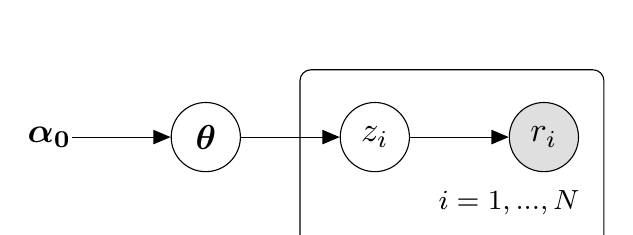
\begin{tikzpicture}[scale=1.25, every node/.style={transform shape}]
        \node[const](alpha){$\bm{\alpha_0}$}; %
        \node[latent, right=of alpha](theta){$\bm{\theta}$}; % 
        \node[latent, right=of theta](z){$z_i$}; %
        \node[obs, right=of z](r){$r_i$}; %
        \edge{alpha}{theta}; %
        \edge{theta}{z}; %
        \edge{z}{r}; %
        \plate[inner sep=0.4cm, xshift = -0.1cm]{plate1}{(z)(r)}{$i=1,...,N$}; %
    \end{tikzpicture}
    \caption[Bayesian graphical model for long-read RNA-seq]{Bayesian graphical model for long-read RNA-seq. Under this model, $\bm\theta$ is a random variable distributed according to $\textrm{Dir}(\bm{\alpha_0})$.}
    \label{fig:graphical-model-2}
\end{figure}
\noindent The posterior probability of the parameters and latent variables given the observed data is 
\begin{equation}\label{eq:post-full}
\begin{split}
    p(\bm{\theta},\bm{Z}\mid\bm{R}) & =\frac{p(\bm{R},\bm{Z},\bm{\theta})}{p(\bm{R})} \\
    & = \frac{p(\bm{R}\mid\bm{Z})\cdot p(\bm{Z}\mid\bm{\theta})\cdot p(\bm{\theta})}{p(\bm{R})} \\
    & = \frac{p(\bm{R}\mid\bm{Z})\cdot p(\bm{Z}\mid\bm{\theta})\cdot p(\bm{\theta})}{\int_\theta \sum_{\bm{Z}} p(\bm{R}\mid\bm{Z})\cdot p(\bm{Z}\mid\bm{\theta})\cdot p(\bm{\theta})\cdot d\theta}
\end{split}
\end{equation}
Direct evaluation of the posterior is intractable, since evaluating the denominator of the final expression in Eq. \ref{eq:post-full} requires summation over the space of $\bm{Z}$, which is exponential ($M^N$) in size. We turn to approximate inference methods for posterior inference. In particular, we consider a variational approximation to the posterior $q(\bm{Z},\bm{\theta})$ that is mean-field, such that the variational distribution factorizes:
\begin{equation}
    q(\bm{Z},\bm{\theta})=q(\bm{Z})\cdot q(\bm\theta)
\end{equation}
Here, we present the optimal variational distributions for $\bm{Z}$ and $\bm\theta$ that minimize the KL divergence to the posterior. Full derivations are presented in Appendix \ref{sec:variational-dist} for brevity. The optimal variational distribution for $\bm{Z}$ is
\begin{equation}\label{eq:opt-z-1}
    q(\bm{Z})=\prod_{i=1}^N\prod_{j=1}^M \gamma_{ij}^{z_{ij}}
\end{equation}
Here, $\gamma_{ij}$ is defined by 
\begin{equation}\label{eq:opt-z-2}
    \gamma_{ij}=\frac{\rho_{ij}}{\sum_j\rho_{ij}}
\end{equation}
with
\begin{equation}\label{eq:opt-z-3}
    \log\rho_{ij}=\log\left[a_{ij}\cdot p(\ell_i\mid d_j,z_{ij}=1)\right]+\psi(\alpha_j)-\psi\left(\sum_{j=1}^M\alpha_j\right)
\end{equation}
where $\psi(\cdot)$ is the digamma function. 
The optimal variational distribution for $\bm\theta$ is
\begin{equation}\label{eq:opt-theta-1}
    q(\bm\theta) = \mathrm{Dir}(\bm\alpha)
\end{equation}
where the $j$\ts{th} component of $\bm\alpha$ is given by
\begin{equation}\label{eq:opt-theta-2}
    \alpha_j=\alpha_{0j}+\sum_{i=1}^N\gamma_{ij}
\end{equation}
From Eqs. \ref{eq:opt-z-1} and \ref{eq:opt-theta-1}, we perform coordinate ascent inference by iteratively optimizing each variational distribution holding the other fixed. This results in an iterative optimization procedure analogous to the EM algorithm:
\begin{enumerate}
    \item Initialize hyperparameters $\alpha_j^{(0)}=\alpha_{0j}$
    \item Update $q(\bm{Z})$: compute $\gamma_{ij}^{(t)}$  with $\alpha_j^{(t)}$ from Eqs. \ref{eq:opt-z-2} and \ref{eq:opt-z-3}
    \item Update $q(\bm\theta)$: compute $\alpha_{j}^{(t+1)}$  with $\gamma_{ij}^{(t)}$ from Eq. \ref{eq:opt-theta-2}
    \item Repeat steps 2 and 3 until convergence. 
\end{enumerate}
Upon convergence, the abundance estimate for the $j$\ts{th} isoform can be obtained by taking the expectation of $\theta_j$ under the posterior distribution:
\begin{equation}
    \mathbb{E}[\theta_j] = \frac{\alpha_{0j}+\sum_i\gamma_{ij}}{\sum_j\alpha_{0j}+N}
\end{equation}

One option for setting hyperparameters $\bm{\alpha_0}$ for the prior $p(\bm{\theta}\mid\bm{\alpha_0})$ is by setting all $\alpha_{0j}$ to some constant $\alpha_0$, yielding a symmetric Dirichlet prior. Small values of $\alpha_0$ result in a sparser $\bm\theta$, while larger values result in a more uniform $\bm\theta$. Another option is to place a hyperprior on $\bm{\alpha_0}$. Since $\bm{\alpha_0}>0$, we can consider
\begin{equation}
    \alpha_{0j}\sim\textrm{Gamma}(a,b)
\end{equation}
We evaluate the choice of priors on transcript quantification in the following section. 



\chapter{Model evaluation and results}

In this chapter, we evaluate our quantification model and inference algorithms on simulated datasets with constant expected degradation rates and real direct RNA-seq datasets with sequencing spike-ins. 

\section{Read alignment}

Simulated and real reads were aligned with minimap2 \cite{Minimap2018, Minimap2021}, a popular aligner for long reads. For alignment to the genome, we used the flags \texttt{-ax splice -uf -k14} that take into account splicing and forward strand alignment for ONT direct RNA-seq as recommended by minimap2 developers. For alignment to the transcriptome, we use default flags \texttt{-ax map-ont -N10} for mapping ONT reads, keeping 10 secondary alignments due to similarities in transcript isoform sequences. We used the same genomic or transcriptomic alignments across the tools, depending on which is required as input.   

\section{Model variations}

We compare two variations of our model based on the read length-isoform agreement:

\paragraph{Deg. EM (exact)} We ran our model with the exact read length-isoform agreement model (Eqn. \ref{eq:read-iso-agreement}) and provided the known degradation rate to the model for inference. This is of course unrealistic, since in real data, the degradation rate is not known \textit{a priori} and there is no bound on the maximum read length (i.e., the degradation rate is not constant). Nevertheless, this serves as a useful sanity check that our approach works. 

\paragraph{Deg. EM (emp.)} The second variation of our model uses the empirical read length-isoform agreement model (Eqn. ) and estimates the degradation rate per base from the data. This variation has no limitation on the maximum read length nor constraints on the degradation rate. 

\section{Methods for benchmarking}

We benchmark our model against three existing methods for transcript quantification from long-read RNA-seq. For brevity, detailed descriptions of these methods are omitted here but included in Appendix \ref{ap:meth}.

\paragraph{Bambu} Bambu (manuscript under review) \cite{Bambu2022} is a method for reference guided transcript discovery and quantification for long read RNA-seq data. Crucially, Bambu is one of the few existing long-read quantification methods that models degradation bias. For benchmarking, we ran Bambu (v.2.0.6) without transcript discovery. For transcript quantification, we ran Bambu with bias correction (default) and without bias correction (\texttt{degradationBias=FALSE}). We used the defaults for all other parameters.

\paragraph{FLAIR} Full-Length Alternative Isoform analysis of RNA (FLAIR) \cite{Tang2020} is a method for correction, isoform definition and alternative splicing analysis of long reads. For benchmarking, we ran FLAIR (v.1.5.1) with the modules \texttt{correct}, \texttt{collapse} and \texttt{quantify}. When running FLAIR on simulated data, we set \texttt{--support 1} for FLAIR \texttt{collapse}, keeping isoforms that are supported by minimally one read (default=3).  

\paragraph{NanoCount} NanoCount \cite{Gleeson2021} is a method for quantifying isoform abundance from ONT direct RNA-seq data. Of the three methods listed here, it is the most comparable to our model as it is tailored for direct RNA-seq and uses an expectation maximization algorithm for estimating isoform abundance estimates. For benchmarking, we ran NanoCount (v.1.0.0.post6) with default parameters.

\section{Evaluations on simulated data}\label{sec:eval-sim}

To evaluate our model's ability to correct for degradation bias, we simulated five datasets for a range of degradation rates $\mathbb{E}[d]\in\{0.05,0.1,0.2,0.4,0.5\}$ (Appendix \ref{ap:sim-deg-reads}). In addition, we simulated reads for artificial novel isoforms that are modified by dropping exons from the 5' end of selected reference isoforms, termed \textit{subset} isoforms (Appendix \ref{ap:gen-novl-iso}, Fig. \ref{fig:app-a-1}). This increases the proportion of multi-mapping reads and makes correcting for degradation bias crucial for accurate transcript quantification. 

The read counts for simulation follow a negative binomial distribution, which is often used for modeling RNA-seq counts and other count data that is over-dispersed, i.e., where the assumption of equal mean and variance is not held \cite{Cameron2013, Anders2010, Robinson2010}. We parameterise the distribution with the mean $\mu$ and a dispersion parameter $\alpha$ such that the variance is given by $\mu+\alpha\mu^2$. This is the same parameterisation used in \cite{Robinson2010}. To ensure that the negative binomial is a valid choice of distribution, we fit discrete distributions to the counts returned by existing methods on real long-read RNA-seq data, and find that the negative binomial provides a better fit to the data compared to the Poisson distribution (Appendix \ref{ap:count-dist}).   

\subsection{Comparisons between model variations}

In this section, we compare the Deg. EM (exact) and Deg. EM (emp.) models based on the isoform abundance estimates obtained. We compare these estimates against the simulated ground truth based on Spearman correlation (SCC), normalized root-mean-squared error (NRMSE) and median relative difference (MRD). Explanations of these metrics can be found in Appendix \ref{ap:eval-metrics}.  

Both variations of the model perform comparably well on the simulated data, achieving SCC $>$ 0.7 across all five simulated datasets with low NRMSE and MRD. Table \ref{tab:summary-1} shows the mean of each metric across the five datasets for all and subset isoforms. We first note that performance on the subset isoforms is poorer compared to that on all isoforms, for both variations and across metrics. This is expected as there is more ambiguity in read assignment with the subset isoforms. 

% Table generated by Excel2LaTeX from sheet 'sec-4-1-table'
\begin{table}[htbp]
\centering
  \resizebox{\columnwidth}{!}{%
\begin{tabular}{|l|P{2cm}|P{2cm}|P{2cm}|P{2cm}|P{2cm}|P{2cm}|}
\cline{2-7}    \multicolumn{1}{c|}{} & \multicolumn{3}{c|}{All isoforms} & \multicolumn{3}{c|}{Subset isoforms} \bigstrut\\
\hline
Method & SCC   & NRMSE & MRD   & SCC   & NRMSE & MRD \bigstrut\\
\hline
Deg. EM (exact) & 0.832 & 0.455 & \textbf{0.006} & \textbf{0.793} & 0.711 & \textbf{0.162} \bigstrut\\
\hline
Deg. EM (emp.) & \textbf{0.852} & \textbf{0.416} & 0.016 & 0.783 & \textbf{0.446} & 0.277 \bigstrut\\
\hline
\end{tabular}%
}
\caption[Summary of metrics across simulated datasets for model variations]{Summary of metrics across simulated datasets for model variations. We report the mean SCC, NRMSE and MRD across the five datasets for all isoforms and subset isoforms separately. Bold values indicate the best performance for each column.}
\label{tab:summary-1}
\end{table}%

Next, we examine the performance on each dataset separately by examining performance on each metric across the datasets for all and subset isoforms (Fig. \ref{fig:4-1-scc-nrmse}). We observe an interesting trend in both the SCC and NRMSE: as the degradation rate increases, the empirical model performs slightly better compared to the exact model. In contrast, the exact model dominates the empirical model in terms of the MRD, especially for subset isoforms.  

To investigate this further, we visualised estimates and fitted a kernel density estimate on the subset isoforms only for datasets with degradation rates 0.2 and 0.5 (Fig. \ref{fig:4-1-scatter}). On a dataset with relatively lower degradation rate (0.2), the exact model performs qualitatively well, with the density of points over the diagonal (Fig. \ref{fig:4-1-scatter}a), while the empirical model underestimates counts for certain isoforms (Fig. \ref{fig:4-1-scatter}b). However, for higher degradation rates (0.5), the exact model appears to aggressively overestimate counts for a subset of isoforms (Fig. \ref{fig:4-1-scatter}c) compared to the empirical model, where the counts are moderately distributed about the diagonal (Fig. \ref{fig:4-1-scatter}d). This explains the significant increase in NRMSE in the exact model for larger degradation rates compared to the empirical model (Fig. \ref{fig:4-1-scc-nrmse}) because the NRMSE penalizes large errors more strongly than moderate errors. 

Based on our analyses in section \ref{sec:deg-est}, we observed that average degradation rates in real direct RNA-seq data tend to be in the range of 0.1-0.2. In this range, the two variations perform comparably, and have a high SCC with each other ($\mathbb{E}[d]$=0.1, SCC=0.957, $\mathbb{E}[d]$=0.2, SCC=0.909).  

\begin{figure}[H]
    \centering
    \includegraphics[width=0.9\textwidth]{figures/sec-4-1-scc-nrmse.png}
    \caption[SCC, NRMSE and MRD across simulated datasets for model variations]{SCC, NRMSE and MRD across simulated datasets for model variations. Here, each point is a dataset with constant expected degradation $\mathbb{E}[d]=\{0.05,0.1,0.2,0.4,0.5\}$. \textbf{a.} SCC on all isoforms. \textbf{b.} SCC on subset isoforms. \textbf{c.} NRMSE on all isoforms. \textbf{d.} NRMSE on subset isoforms. \textbf{f.} MRD on all isoforms. \textbf{e.} MRD on subset isoforms.}
    \label{fig:4-1-scc-nrmse}
\end{figure}

\begin{figure}[H]
    \centering
    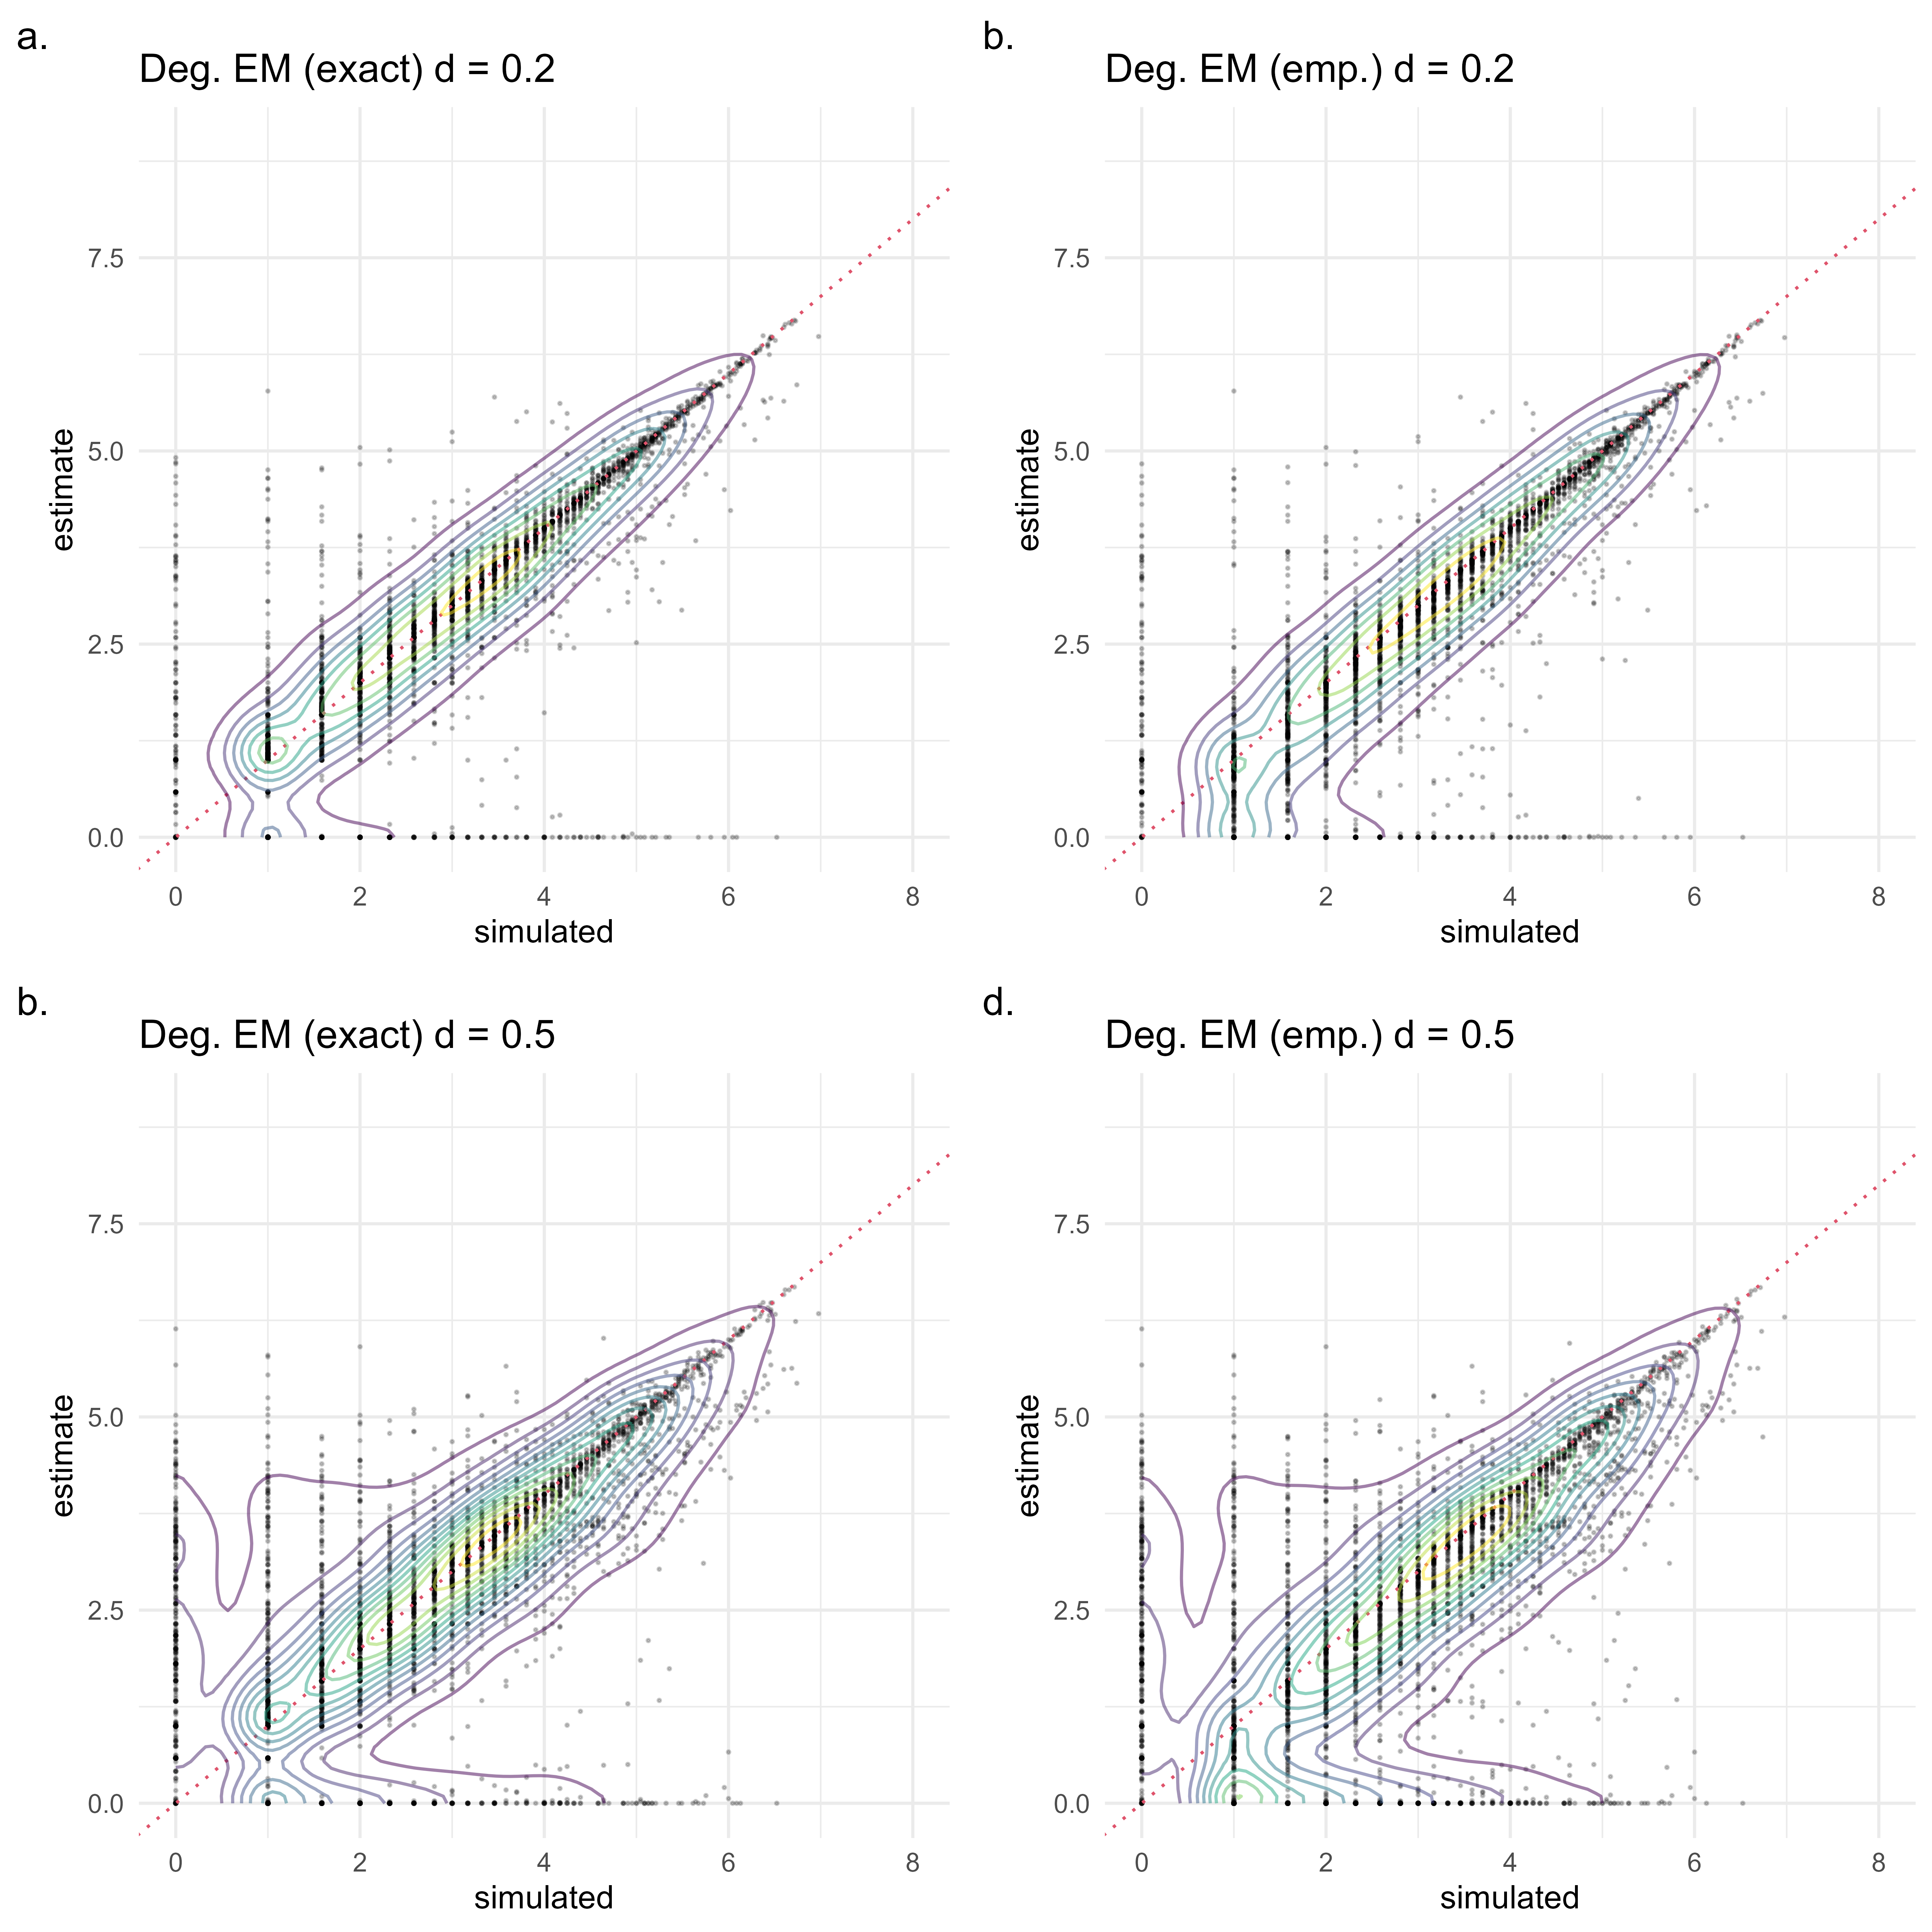
\includegraphics[width=\textwidth]{figures/sec-4-1-scatter-hard.png}
    \caption[Scatter plots across simulated datasets for model variations]{Scatter plots of the simulated and estimated counts on the log2 scale across simulated datasets with $\mathbb{E}[d]=0.2$ and $\mathbb{E}[d]=0.5$ for the exact and empirical model. \textbf{a.} Exact model with degradation 0.2. \textbf{b.} Empirical model with degradation 0.2. \textbf{c.} Exact model with degradation 0.5. \textbf{d.} Empirical model with degradation 0.5.}
    \label{fig:4-1-scatter}
\end{figure}

\subsection{Comparisons with existing methods}

We now benchmark our model against Bambu with and without bias modeling, FLAIR and NanoCount by comparing the estimates returned by each method with the simulated ground truth. We analyse counts for all isoforms that we included in the simulation and where the sum of counts across the methods was greater than zero. In addition, we make a distinction between methods that are \textit{bias-aware} (Deg. EM (exact), Deg. EM (emp.), Bambu) and methods that are \textit{bias-unaware} (Bambu (no bias), FLAIR, NanoCount). 

All methods perform reasonably well on the simulated data across all isoforms, achieving SCC $>$ 0.69 across all five simulated datasets (Table \ref{tab:summary-2}). NRMSE across the methods are comparable, but MRD for the other methods are about one order of magnitude larger than those attained by our model. However, we observe stark differences between the bias-aware and bias-unaware methods on the subset isoforms. In particular, bias-unaware methods perform considerably poorer on SCC and MRD than bias-aware ones (Table \ref{tab:summary-2}).    

\begin{table}[htbp]
\centering
\resizebox{\columnwidth}{!}{%
\begin{tabular}{|l|P{2cm}|P{2cm}|P{2cm}|P{2cm}|P{2cm}|P{2cm}|}
\cline{2-7}    \multicolumn{1}{r|}{} & \multicolumn{3}{c|}{All isoforms} & \multicolumn{3}{c|}{Subset isoforms} \bigstrut\\
\hline
Method & SCC   & NRMSE & MRD   & SCC   & NRMSE & MRD \bigstrut\\
\hline
Deg. EM (exact) & 0.845 & 0.449 & \textbf{0.002} & \textbf{0.815} & 0.699 & \textbf{0.135} \bigstrut\\
\hline
Deg. EM (emp.) & \textbf{0.863} & \textbf{0.41} & 0.012 & 0.801 & \textbf{0.439} & 0.241 \bigstrut\\
\hline
Bambu & 0.771 & 0.599 & 0.101 & 0.671 & 1.009 & 0.36 \bigstrut\\
\hline
Bambu (no bias) & 0.739 & 0.637 & 0.107 & 0.432 & 1.165 & 0.926 \bigstrut\\
\hline
FLAIR & 0.696 & 0.697 & 0.081 & 0.153 & 1.176 & 0.974 \bigstrut\\
\hline
NanoCount & 0.759 & 0.566 & 0.105 & 0.408 & 1.056 & 0.931 \bigstrut\\
\hline
\end{tabular}%
}
\caption[Summary of metrics across simulated datasets for different methods]{Summary of metrics across simulated datasets for different methods. We report the mean SCC, NRMSE and MRD across the five datasets for all isoforms and subset isoforms separately. Bold values indicate the best performance for each column.}
\label{tab:summary-2}
\end{table}%

Next, we examine the performance on each dataset separately for all the methods on all and subset isoforms separately (Fig. \ref{fig:4-2-scc-nrmse}). Both Deg. EM (exact) and Deg. EM (empirical) show better performance on all metrics compared to other methods across the datasets. We also note that Bambu with bias modeling improves the performance over Bambu without bias modeling across the whole range of degradation rates. In addition, Bambu's performance drops quickly as the degradation rate increases, as its degradation rate is purposefully calibrated or moderated to lower degradation rates. The authors note that this is to allow for comparisons across samples or replicates, as correction for different degradation rates across samples may result in technical variation which impact downstream analyses. We examine this claim based on reproducibility metrics on real data in the following section. For degradation rates commonly observed in real data (0.1-0.2), Bambu performs better compared to FLAIR and NanoCount on both SCC and NRMSE (Fig. \ref{fig:4-1-scc-nrmse}a,c). 

Bias-unaware methods perform poorly over the subset isoforms across the whole range of degradation rates. Interestingly, the MRD on subset isoforms for bias-unaware methods remained consistently high and was invariant across the range of degradation rates, while for bias-aware methods, the MRD was always lower compared to bias-unaware methods and increased with the degradation rate (\ref{fig:4-2-scc-nrmse}e). This demonstrates the importance of bias correction and illustrates the difficulty of correcting for degradation bias when the degradation rate is high.     

\newpage

\begin{figure}[H]
    \centering
    \includegraphics[width=0.9\textwidth]{figures/sec-4-2-scc-nrmse.png}
    \caption[SCC, NRMSE and MRD across simulated datasets for different methods]{SCC, NRMSE and MRD across simulated datasets for different methods. Here, each point is a dataset with constant expected degradation $\mathbb{E}[d]=\{0.05,0.1,0.2,0.4,0.5\}$. \textbf{a.} SCC on all isoforms. \textbf{b.} SCC on subset isoforms. \textbf{c.} NRMSE on all isoforms. \textbf{d.} NRMSE on subset isoforms. \textbf{f.} MRD on all isoforms. \textbf{e.} MRD on subset isoforms.}
    \label{fig:4-2-scc-nrmse}
\end{figure}

\newpage

\begin{figure}[H]
    \centering
    \includegraphics[width=0.9\textwidth]{figures/sec-4-2-scatter-hard.png}
    \caption[Scatter plots across simulated datasets for different methods]{Scatter plots of the simulated and estimated counts on the log2 scale across simulated datasets with $\mathbb{E}[d]=0.2$ for all methods. \textbf{a.} Deg. EM (exact) model. \textbf{b.} Deg. EM (emp.) model. \textbf{c.} Bambu with bias modeling. \textbf{d.} Bambu with no bias modeling. \textbf{e.} FLAIR. \textbf{f.} NanoCount.}
    \label{fig:4-2-scatter}
\end{figure}

\newpage

Finally, we visualised estimates and fitted a kernel density estimate on the subset isoforms for all methods on the dataset with a degradation rate of 0.2 (Fig. \ref{fig:4-2-scatter}), which we observe to be common in real data. On this dataset, bias-aware methods significantly improve over bias-unaware ones qualitatively (Fig. \ref{fig:4-2-scatter}a,b,c). In particular, without correcting for bias, Bambu (no bias), FLAIR and NanoCount (Fig. \ref{fig:4-2-scatter}d,e,f) severely underestimate the counts for subset isoforms to different extents, with FLAIR performing the worst.

\subsection{Runtime analysis}

We measured the end-to-end runtime taken for all methods (Fig. \ref{fig:runtime}) excluding the read alignment step. Bambu and FLAIR were run with 12 threads, while NanoCount and the current verison of our model do not implement parallelisation. Across the five datasets, NanoCount was the fastest, followed by Deg. EM (exact). Bambu and FLAIR performed similarly, though FLAIR had a much larger variance in the runtime. Even though the time complexity for both Deg. EM (exact) and Deg. EM (emp.) is $\mathcal{O}(N_A)$, where $N_A$ is the number of alignments, Deg. EM (emp.) is much slower than all other methods because calculation of the empirical read length-isoform agreement probabilities is computationally intensive. Even though the runtimes for the empirical model are longer, they are still tolerable in absolute terms, and come with improvements in accuracy for accurately quantifying degraded reads. Nevertheless, this is one area for improvement for future iterations of our model.  

\begin{figure}[H]
    \centering
    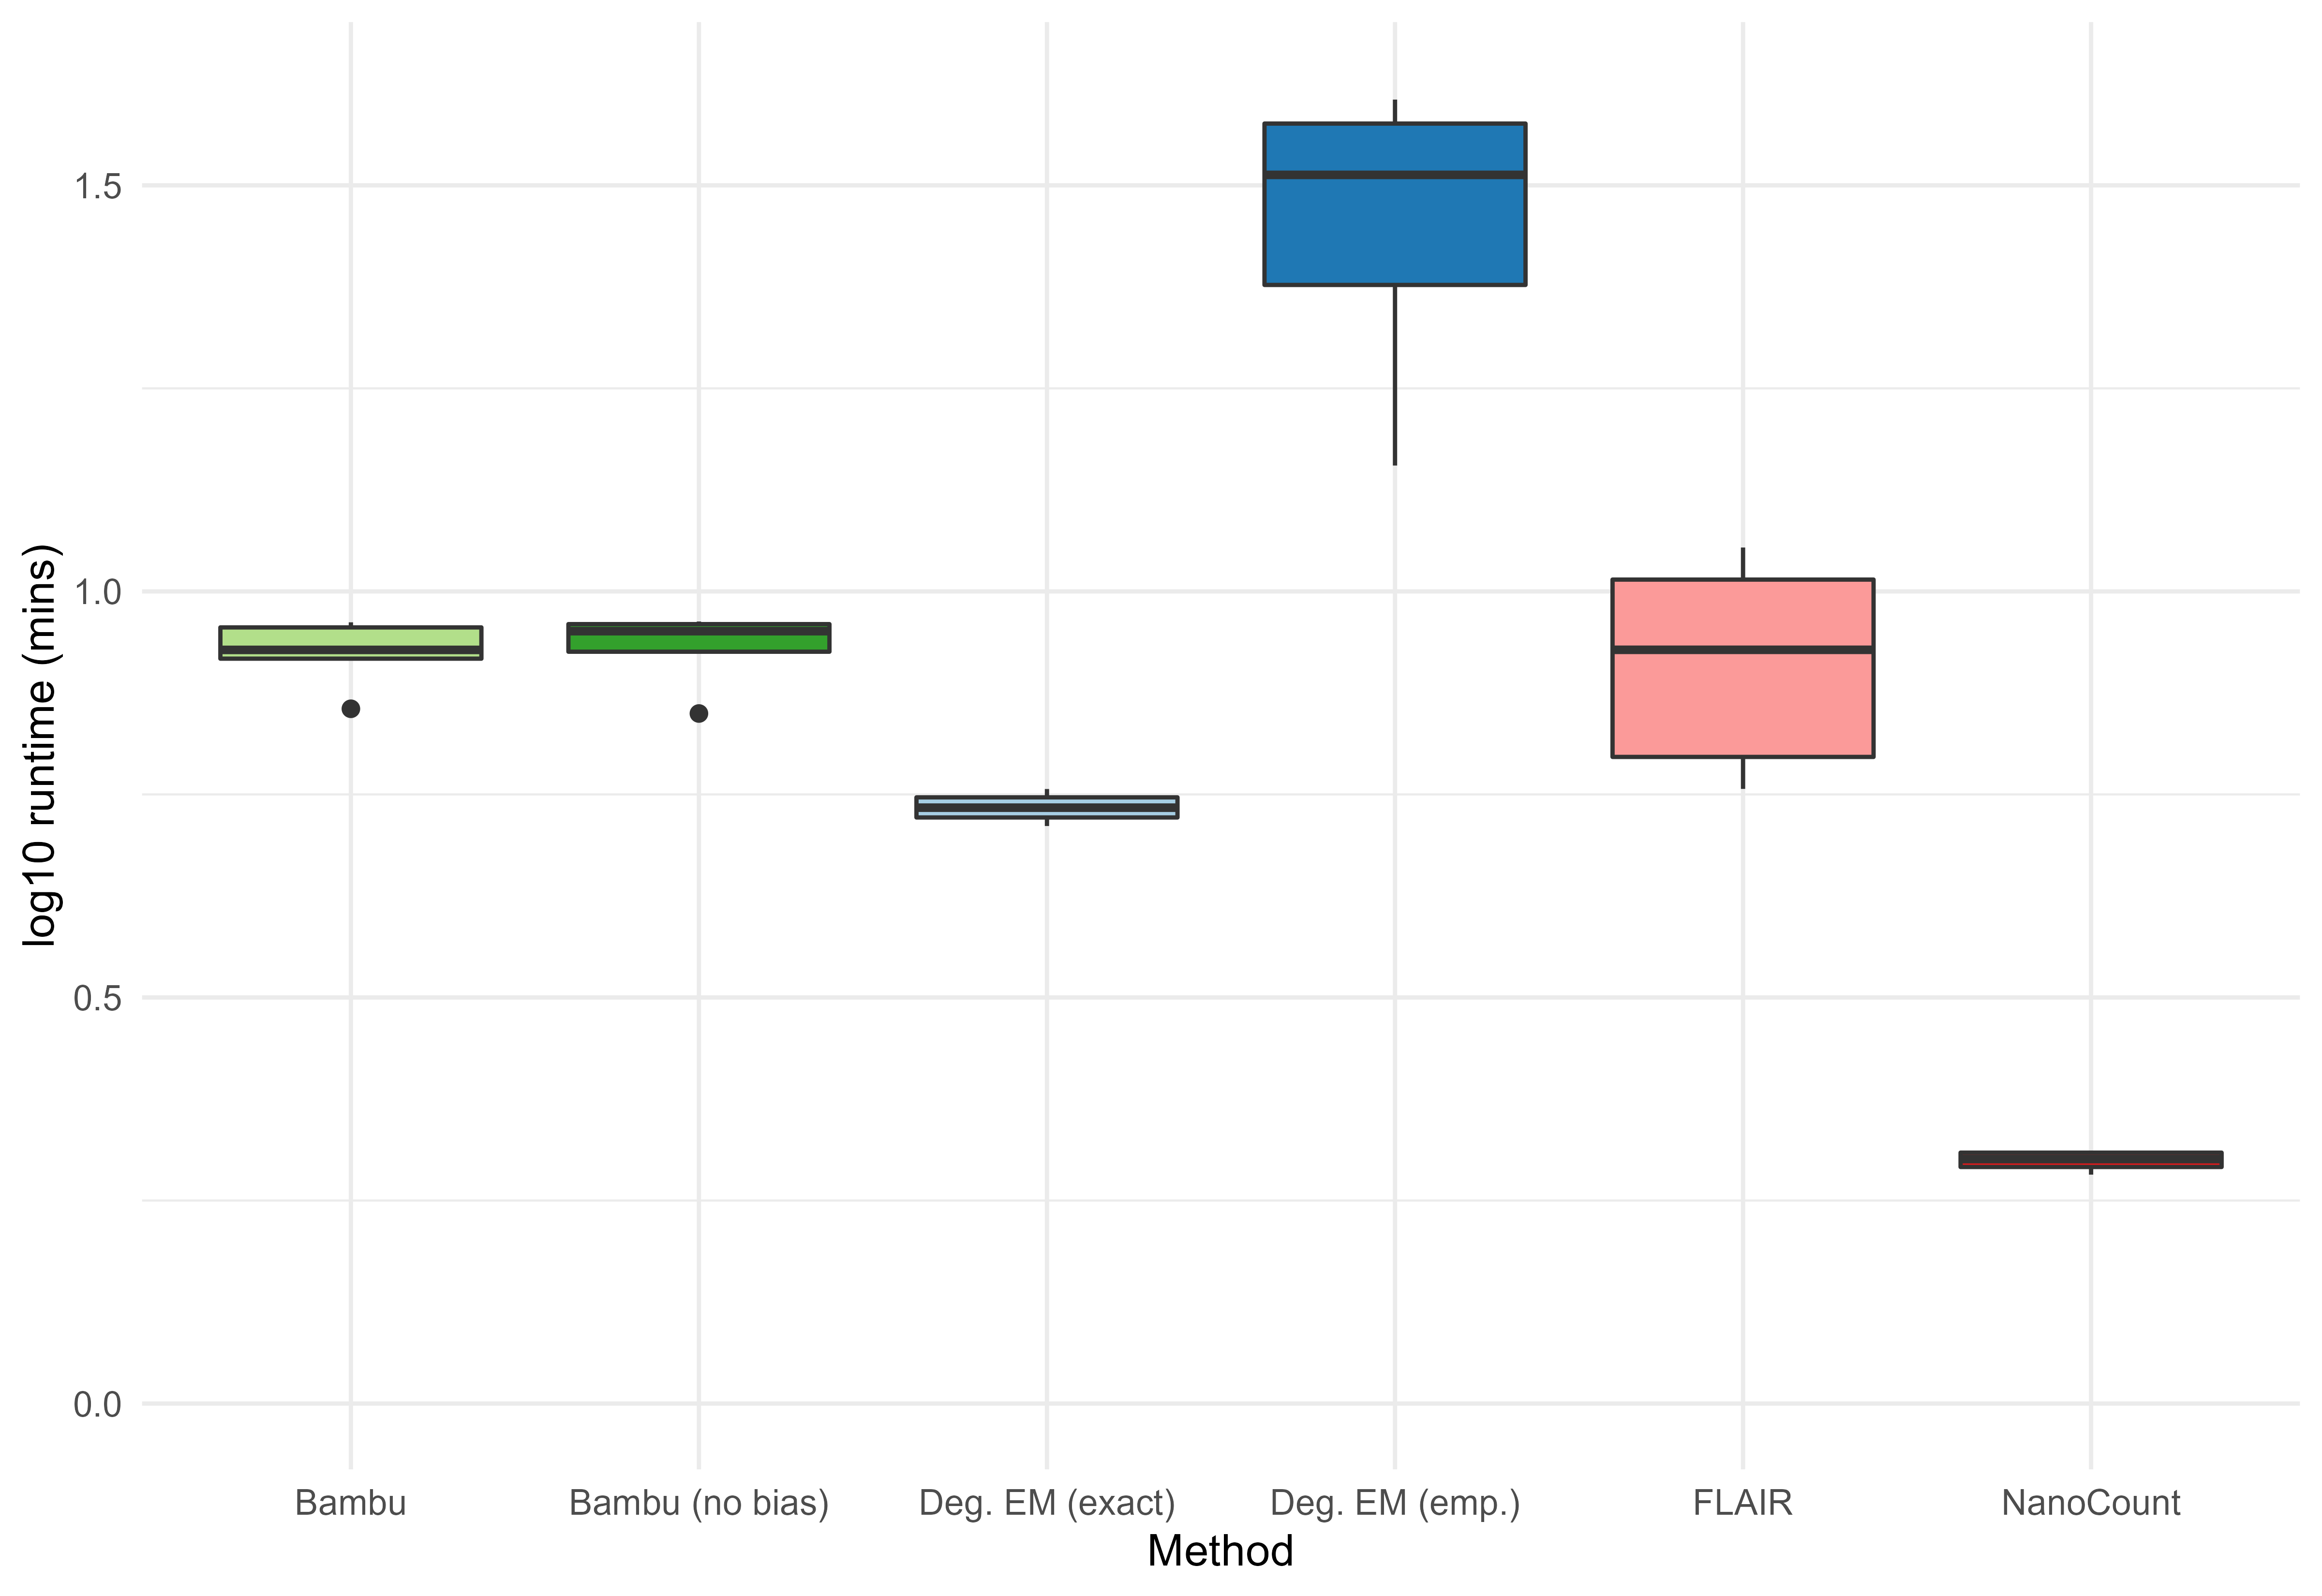
\includegraphics[width=0.825\textwidth]{figures/sec-4-runtime.png}
    \caption[Runtime across simulated datasets for different methods]{Runtime (mins) across simulated datasets for different methods. Times are log10 transformed.}
    \label{fig:runtime}
\end{figure}

\section{Evaluations on real data}

In this section, we evaluate Deg. EM (emp.), Bambu with bias modeling, and NanoCount on direct RNA-seq data with  from the SG-NEx project. In particular, we examine the performance of these methods on samples containing RNA sequencing spike-ins (Table \ref{tab-sgnex}). A subset of samples contain Spike-In RNA Variants (SIRVs) \cite{Lexogen20201} while another contain RNA sequins \cite{Sequins} (See Appendix \ref{ap-spike} for more details). The expression of these spike-ins are supposedly known and can be used as a reference.   

\begin{table}[htbp]
  \centering
    \begin{tabular}{|p{2cm}|p{2cm}|p{2cm}|p{3.5cm}|}
    \hline
    Cell Line & Run & Replicate   & Spike-in \bigstrut\\
    \hline
    Hct116 & 1     & 3     & Sequin Mix A v1.0 \bigstrut\\
    \hline
    K562  & 1     & 4     & Sequin Mix A v1.0 \bigstrut\\
    \hline
    K562  & 1     & 5   & Sequin Mix A v1.0 \bigstrut\\
    \hline
    MCF7  & 1     & 4     & Sequin Mix A v1.0 \bigstrut\\
    \hline
    H9    & 1     & 2     & SIRV-4 \bigstrut\\
    \hline
    H9    & 1     & 3     & SIRV-4 \bigstrut\\
    \hline
    H9    & 1     & 4     & SIRV-4 \bigstrut\\
    \hline
    H9    & 2     & 2     & SIRV-4 \bigstrut\\
    \hline
    H9    & 2     & 3     & SIRV-4 \bigstrut\\
    \hline
    H9    & 2     & 4     & SIRV-4 \bigstrut\\
    \hline
    \end{tabular}%
  \caption[Description of SG-NEx direct RNA-seq samples.]{Description of SG-NEx direct RNA-seq samples. A subset of samples is spiked-in with Sequins while another is spiked-in with SIRV-4.}
  \label{tab-sgnex}
\end{table}%

\subsection{Empirical results on spike-ins}

First, we examine results on the RNA sequin spike-ins (n=41 transcripts). For each of the four samples, we computed the SCC, NRMSE and MRD on the abundance estimates returned by each method (Fig. \ref{fig:sequin-metrics}). Deg. EM (emp.) achieved the highest median SCC, while NanoCount perform reasonably well with a median SCC $>$ 0.7. Bambu's performance was weighed down by an outlier (Fig. \ref{fig:sequin-metrics}a). NRMSE and MRD metrics show similar trends, with Deg. EM (emp.) achieving the lowest median NRMSE and MRD (Fig. \ref{fig:sequin-metrics}b,c).

We visualize the estimates and supposed concentrations of the sequins for the sample K562 replicate 5 run 1 (Fig \ref{fig:sequin-scatter}) which obtained close to median performance across the metrics for all methods. Qualitatively, Deg. EM and NanoCount achieve similar results, though in the latter, there is a slight overestimation of counts. Bambu underestimates the counts for a subset of lowly expressed sequins that results in a decrease in performance over the three metrics.  

\begin{figure}[H]
    \centering
    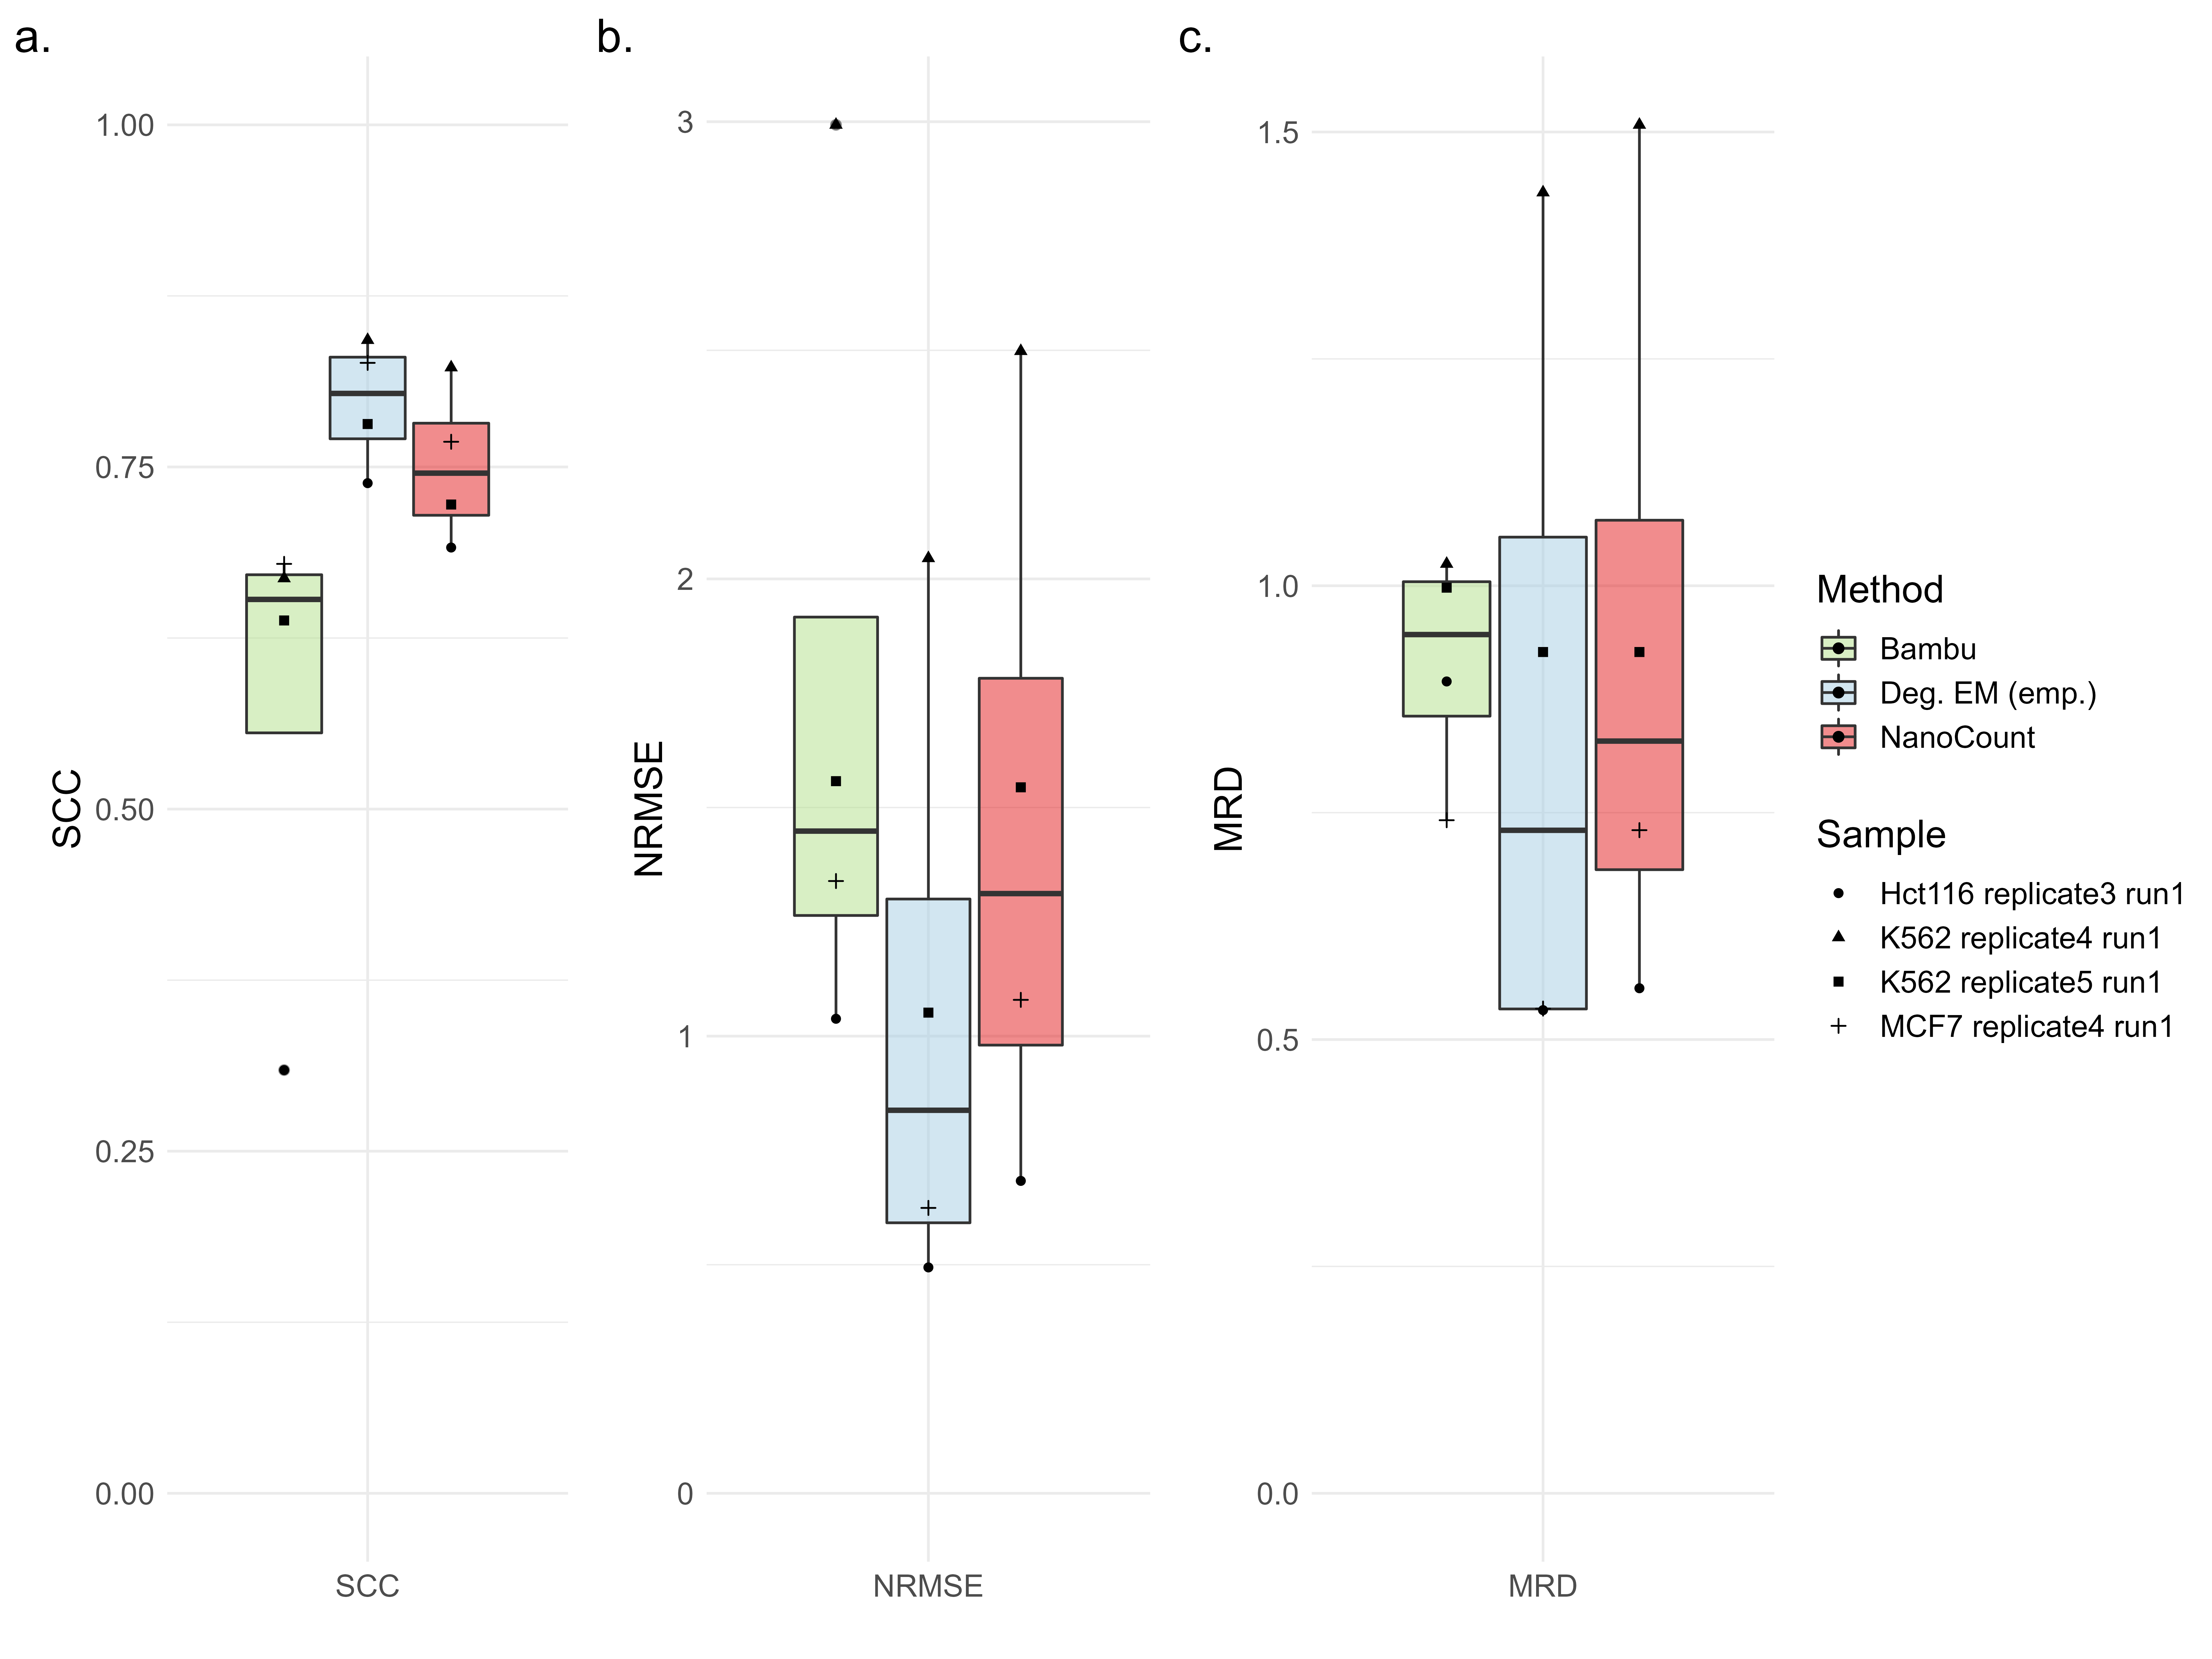
\includegraphics[width=\textwidth]{figures/sequin-metrics.png}
    \caption[SCC, NRMSE and MRD on RNA sequins in SG-NEx data]{SCC, NRMSE and MRD on RNA sequins in SG-NEx data. \textbf{a.} SCC, \textbf{b.} NRMSE and \textbf{c.} MRD for each of the three methods across four samples.}
    \label{fig:sequin-metrics}
\end{figure}

\begin{figure}[H]
    \centering
    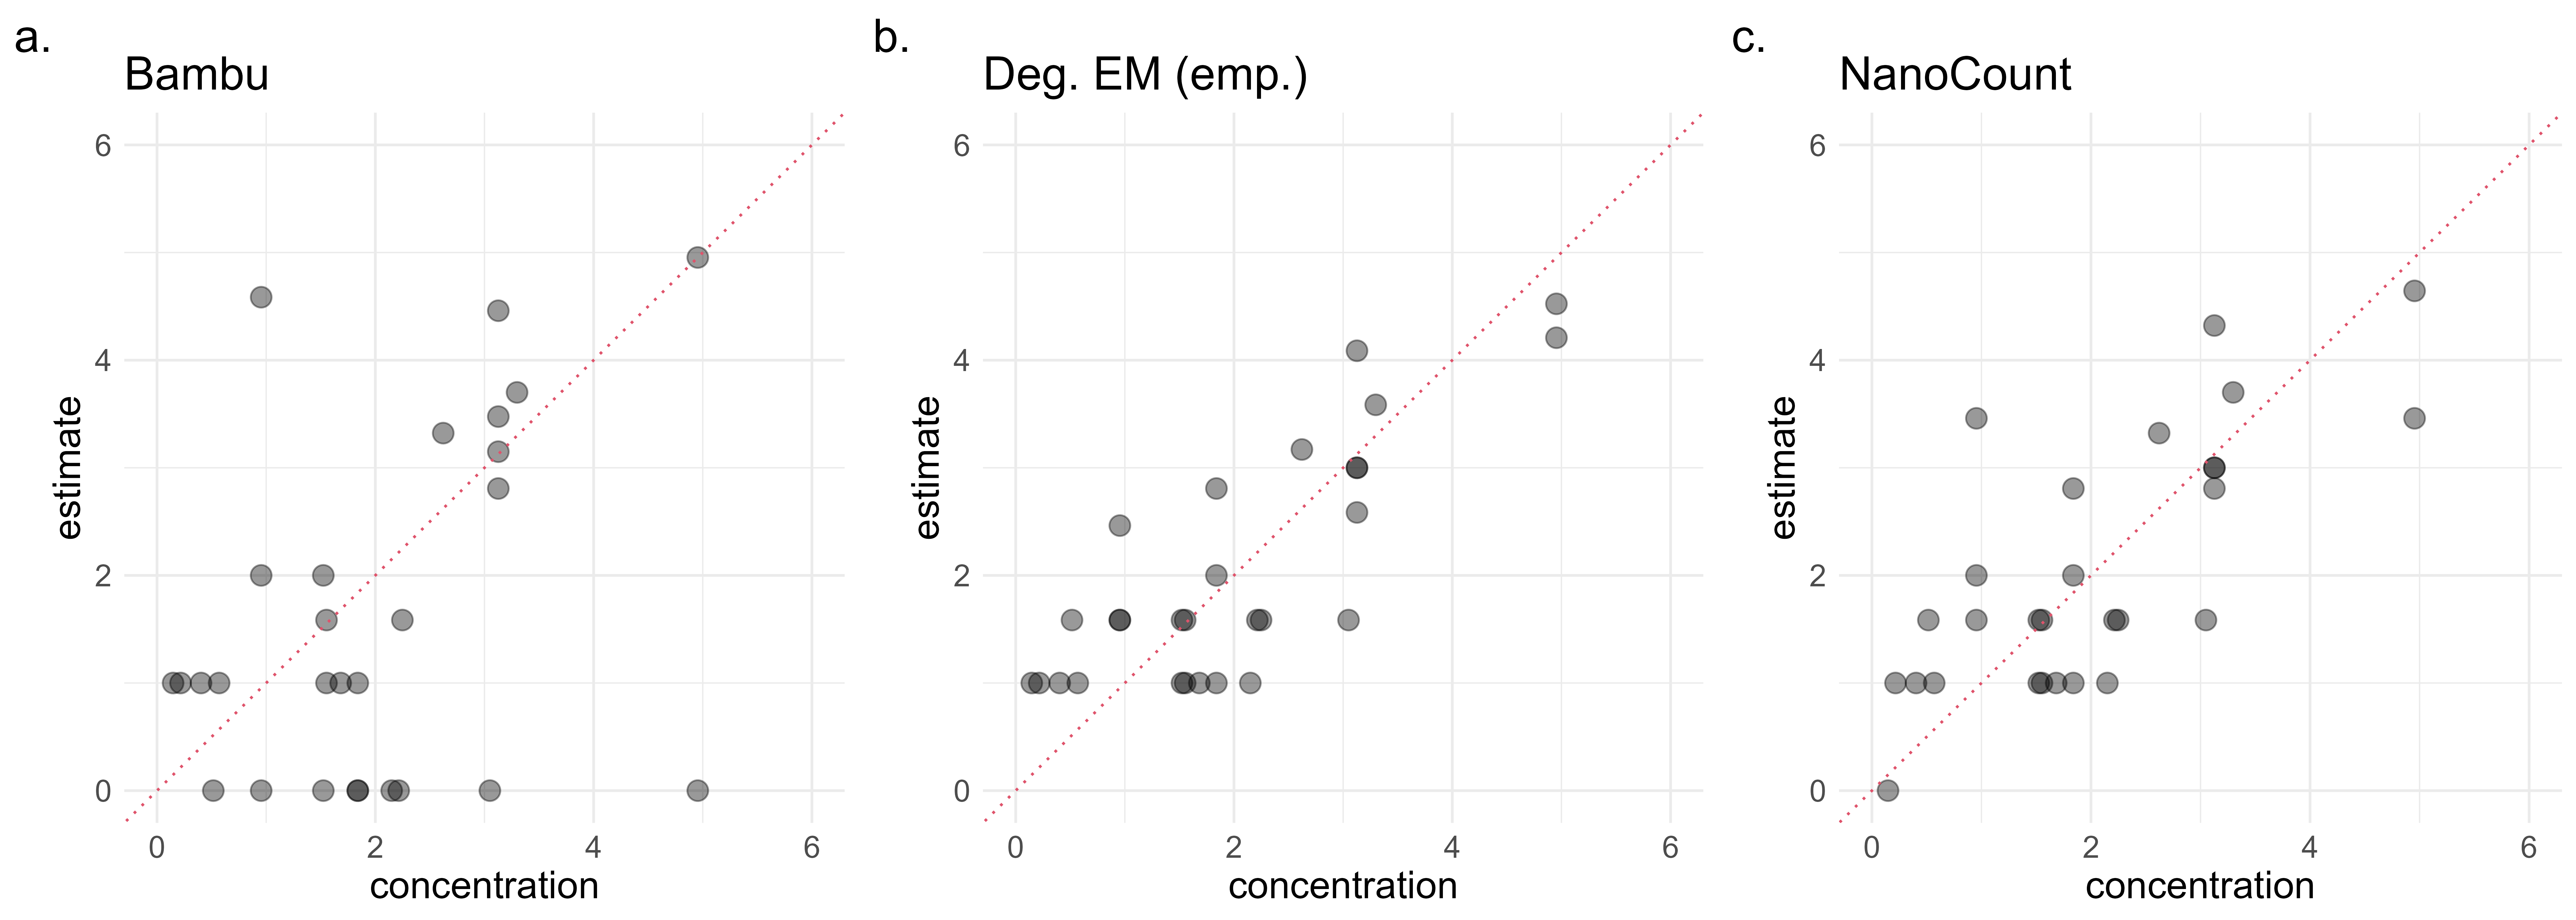
\includegraphics[width=\textwidth]{figures/sequin-scatter.png}
    \caption[Scatter plots on RNA sequins in SG-NEx data]{Scatter plots on RNA sequins in sample K562 replicate 5 run 1 for \textbf{a.} Bambu, \textbf{b.} Deg. EM (emp.) and \textbf{c.} NanoCount. Plots for rest of the samples are qualitatively similar.}
    \label{fig:sequin-scatter}
\end{figure}

\begin{figure}[H]
    \centering
    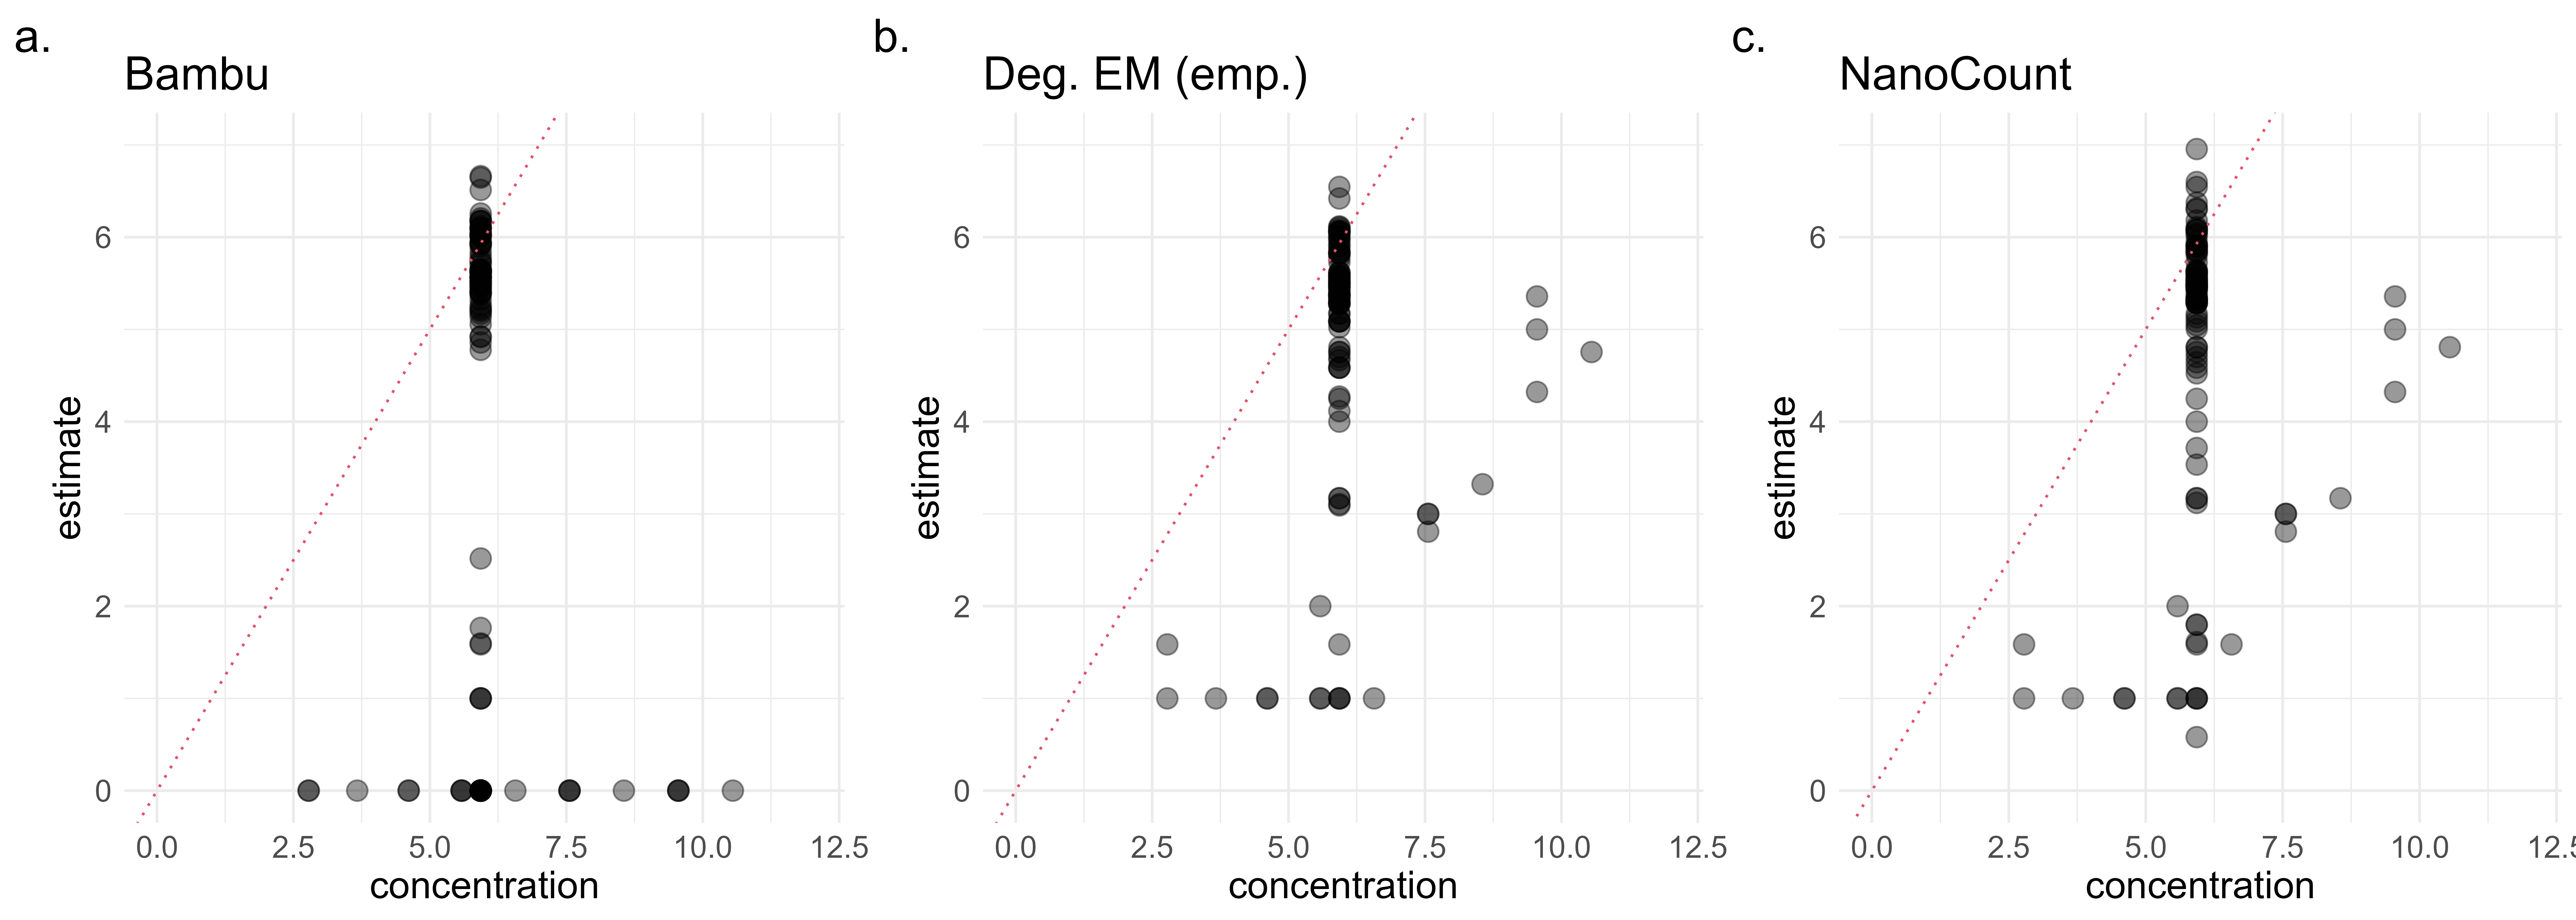
\includegraphics[width=\textwidth]{figures/lexogen-scatter.png}
    \caption[Scatter plots on SIRVs in SG-NEx data]{Scatter plots on SIRVs in SG-NEx data in H9 replicate 4 run 1 for \textbf{a.} Bambu, \textbf{b.} Deg. EM (emp.) and \textbf{c.} NanoCount. Plots for rest of the samples are qualitatively similar.}
    \label{fig:lexogen-scatter}
\end{figure}

\begin{figure}[H]
    \centering
    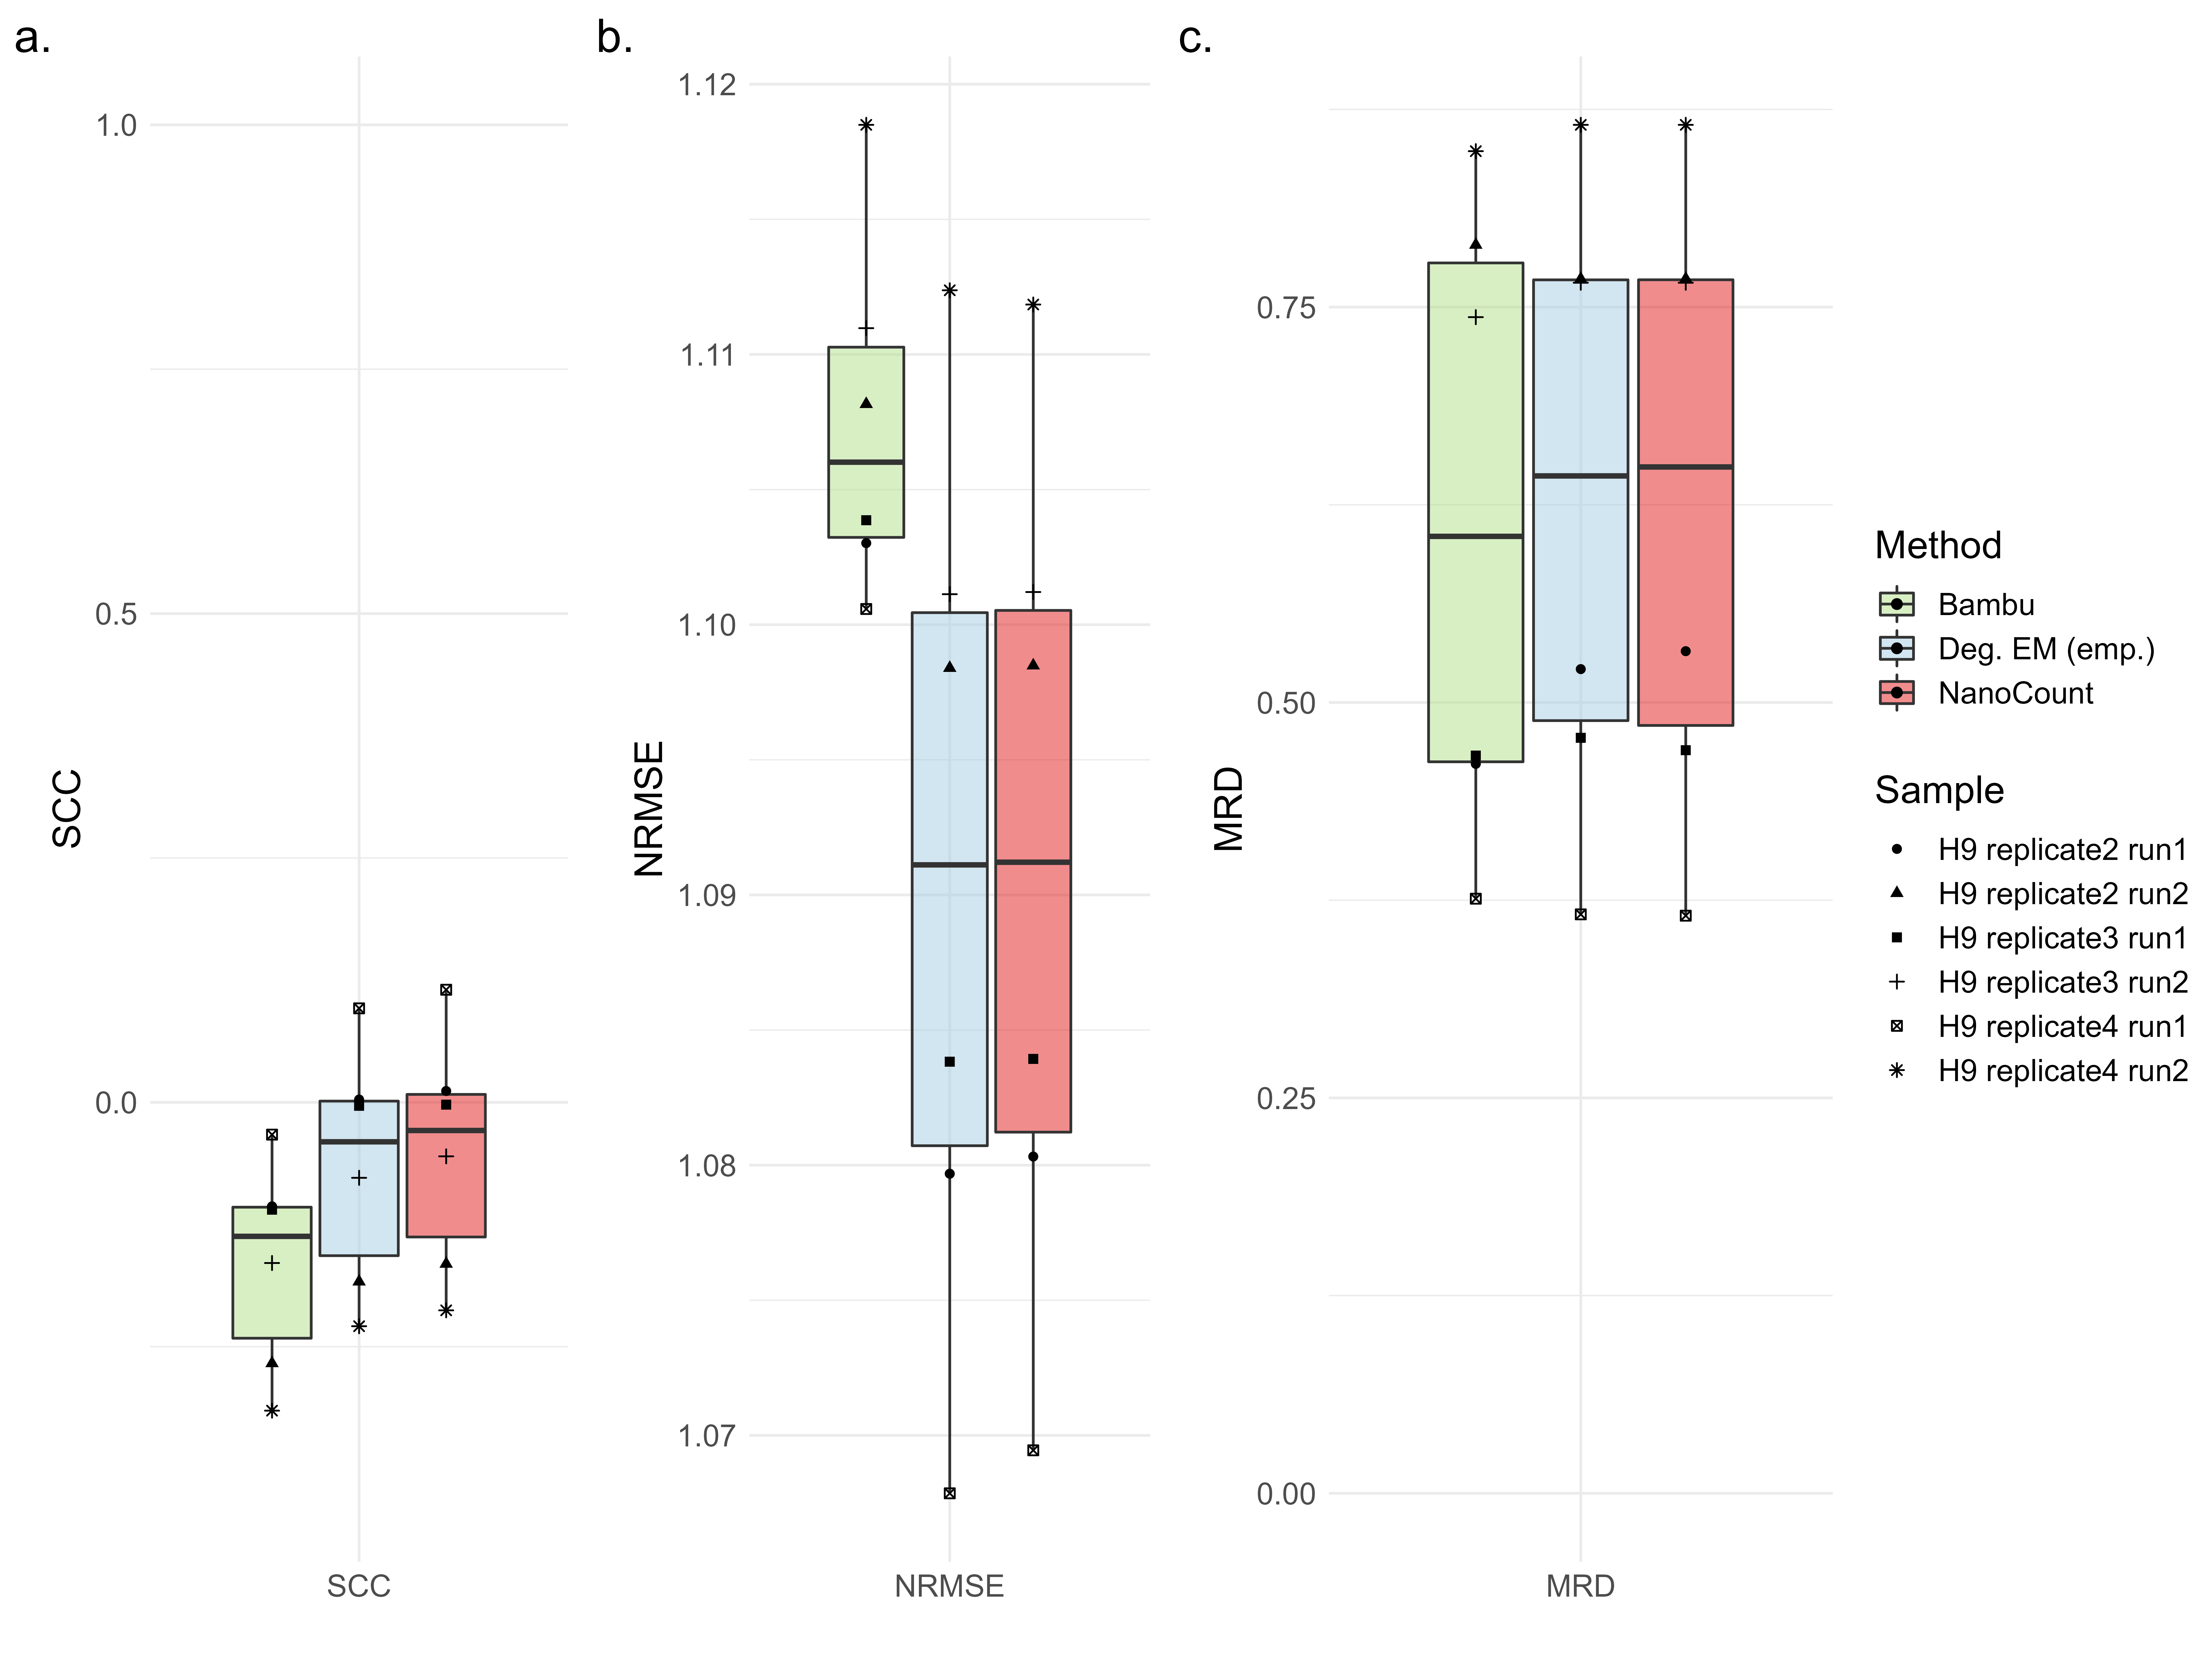
\includegraphics[width=\textwidth]{figures/lexogen.png}
    \caption[SCC, NRMSE and MRD on SIRVs in SG-NEx data]{SCC, NRMSE and MRD on SIRV-4 in SG-NEx data. \textbf{a.} SCC, \textbf{b.} NRMSE and \textbf{c.} MRD for each of the three methods across six H9 samples.}
    \label{fig:lexogen-metrics}
\end{figure}

In addition to the sequin spike-in samples, we examined the SIRV spike-ins in six H9 direct RNA-seq samples (Table \ref{tab-sgnex}). For all methods and across the samples, the abundance estimates for SIRVs did not reflect the supposed concentration (Fig. \ref{fig:lexogen-scatter}). However, the estimates obtained across the methods correlated well with each other (median of median pairwise SCC = 0.806, p-value $<$ 2.2e-16). This might suggest that the supposed SIRV concentrations do not accurately represent what is actually present in the samples, diminishing their utility as a control for RNA-seq in this context. Nevertheless, we computed the SCC, NRMSE and MRD across the six samples for each method (Fig. \ref{fig:lexogen-metrics}). The performance on all metrics is similar across the methods, but is unlikely to be informative due to reasons discussed above.   

\section{Reproducibilty measures}

Besides quantifying accuracy, we can also measure the reproducibility of abundance estimates for each method. We do so with the reproducibility metric (RM), which is a measure of the standard deviation of abundance estimates across replicates (Appendix \ref{ap:eval-metrics}). We use H9 samples in the SG-NEx data that were sequenced in two runs, with three replicates in each run (Table \ref{tab-sgnex}). Within each run, we calculated the RM across the replicates for each isoform called as expressed in at least one method and obtained the median reproducibiltiy metric (MRM) (Table \ref{tab-mrm}). For all methods, MRM in the first run was higher than that in the second by virtue of the number of isoforms the MRM was calculated over (Run 1 = 30,720, Run 2 = 21,536). In both runs, Deg. EM (emp.) achieved the lowest MRM suggesting higher reproducibility compared to NanoCount or Bambu. 

\begin{table}[htbp]
\centering
\begin{tabular}{|p{3cm}|p{2cm}|p{2cm}|}
\hline
Method & Run 1 & Run 2 \bigstrut\\
\hline
Deg. EM (emp.) & \textbf{0.904} & \textbf{0.812} \bigstrut\\
\hline
Bambu & 1.193 & 0.943 \bigstrut\\
\hline
NanoCount & 0.943 & 0.816 \bigstrut\\
\hline
\end{tabular}%
\caption[MRM across different runs for SG-NEx data]{MRM across different runs for SG-NEx H9 samples.}
\label{tab-mrm}%
\end{table}%

The incorporation of bias modeling in Deg. EM improves reproducibility. We can infer this by comparing the MRMs obtained by Deg. EM and NanoCount, which Deg. EM can most closely be compared to. By modeling the bias, read-to-isoform assignment is improved across replicates with potentially different degradation rates, thus stabilising variance in abundance estimates across the replicates.       

\section{Comparisons of estimated degradation}

Lastly, we compare the estimated average degradation rates obtained by Bambu and Deg. EM (emp.) across samples from four cell lines. We note that we do not expect the absolute values of the degradation rates to be similar; rather, we expect the estimates to be linearly related. Indeed, by fitting a regressing the estimates from Bambu against Deg. EM (Fig. \ref{fig:real-deg-rate}) in a linear model, we find that the linear relationship is significant (p-value = 2.63e-05, adjusted $R^2$ = 0.890). Even though the sample size here is small, the concordance between the degradation rates estimated by Bambu and Deg. EM (emp.) on real data provides a useful sanity check for our model.

\begin{figure}
    \centering
    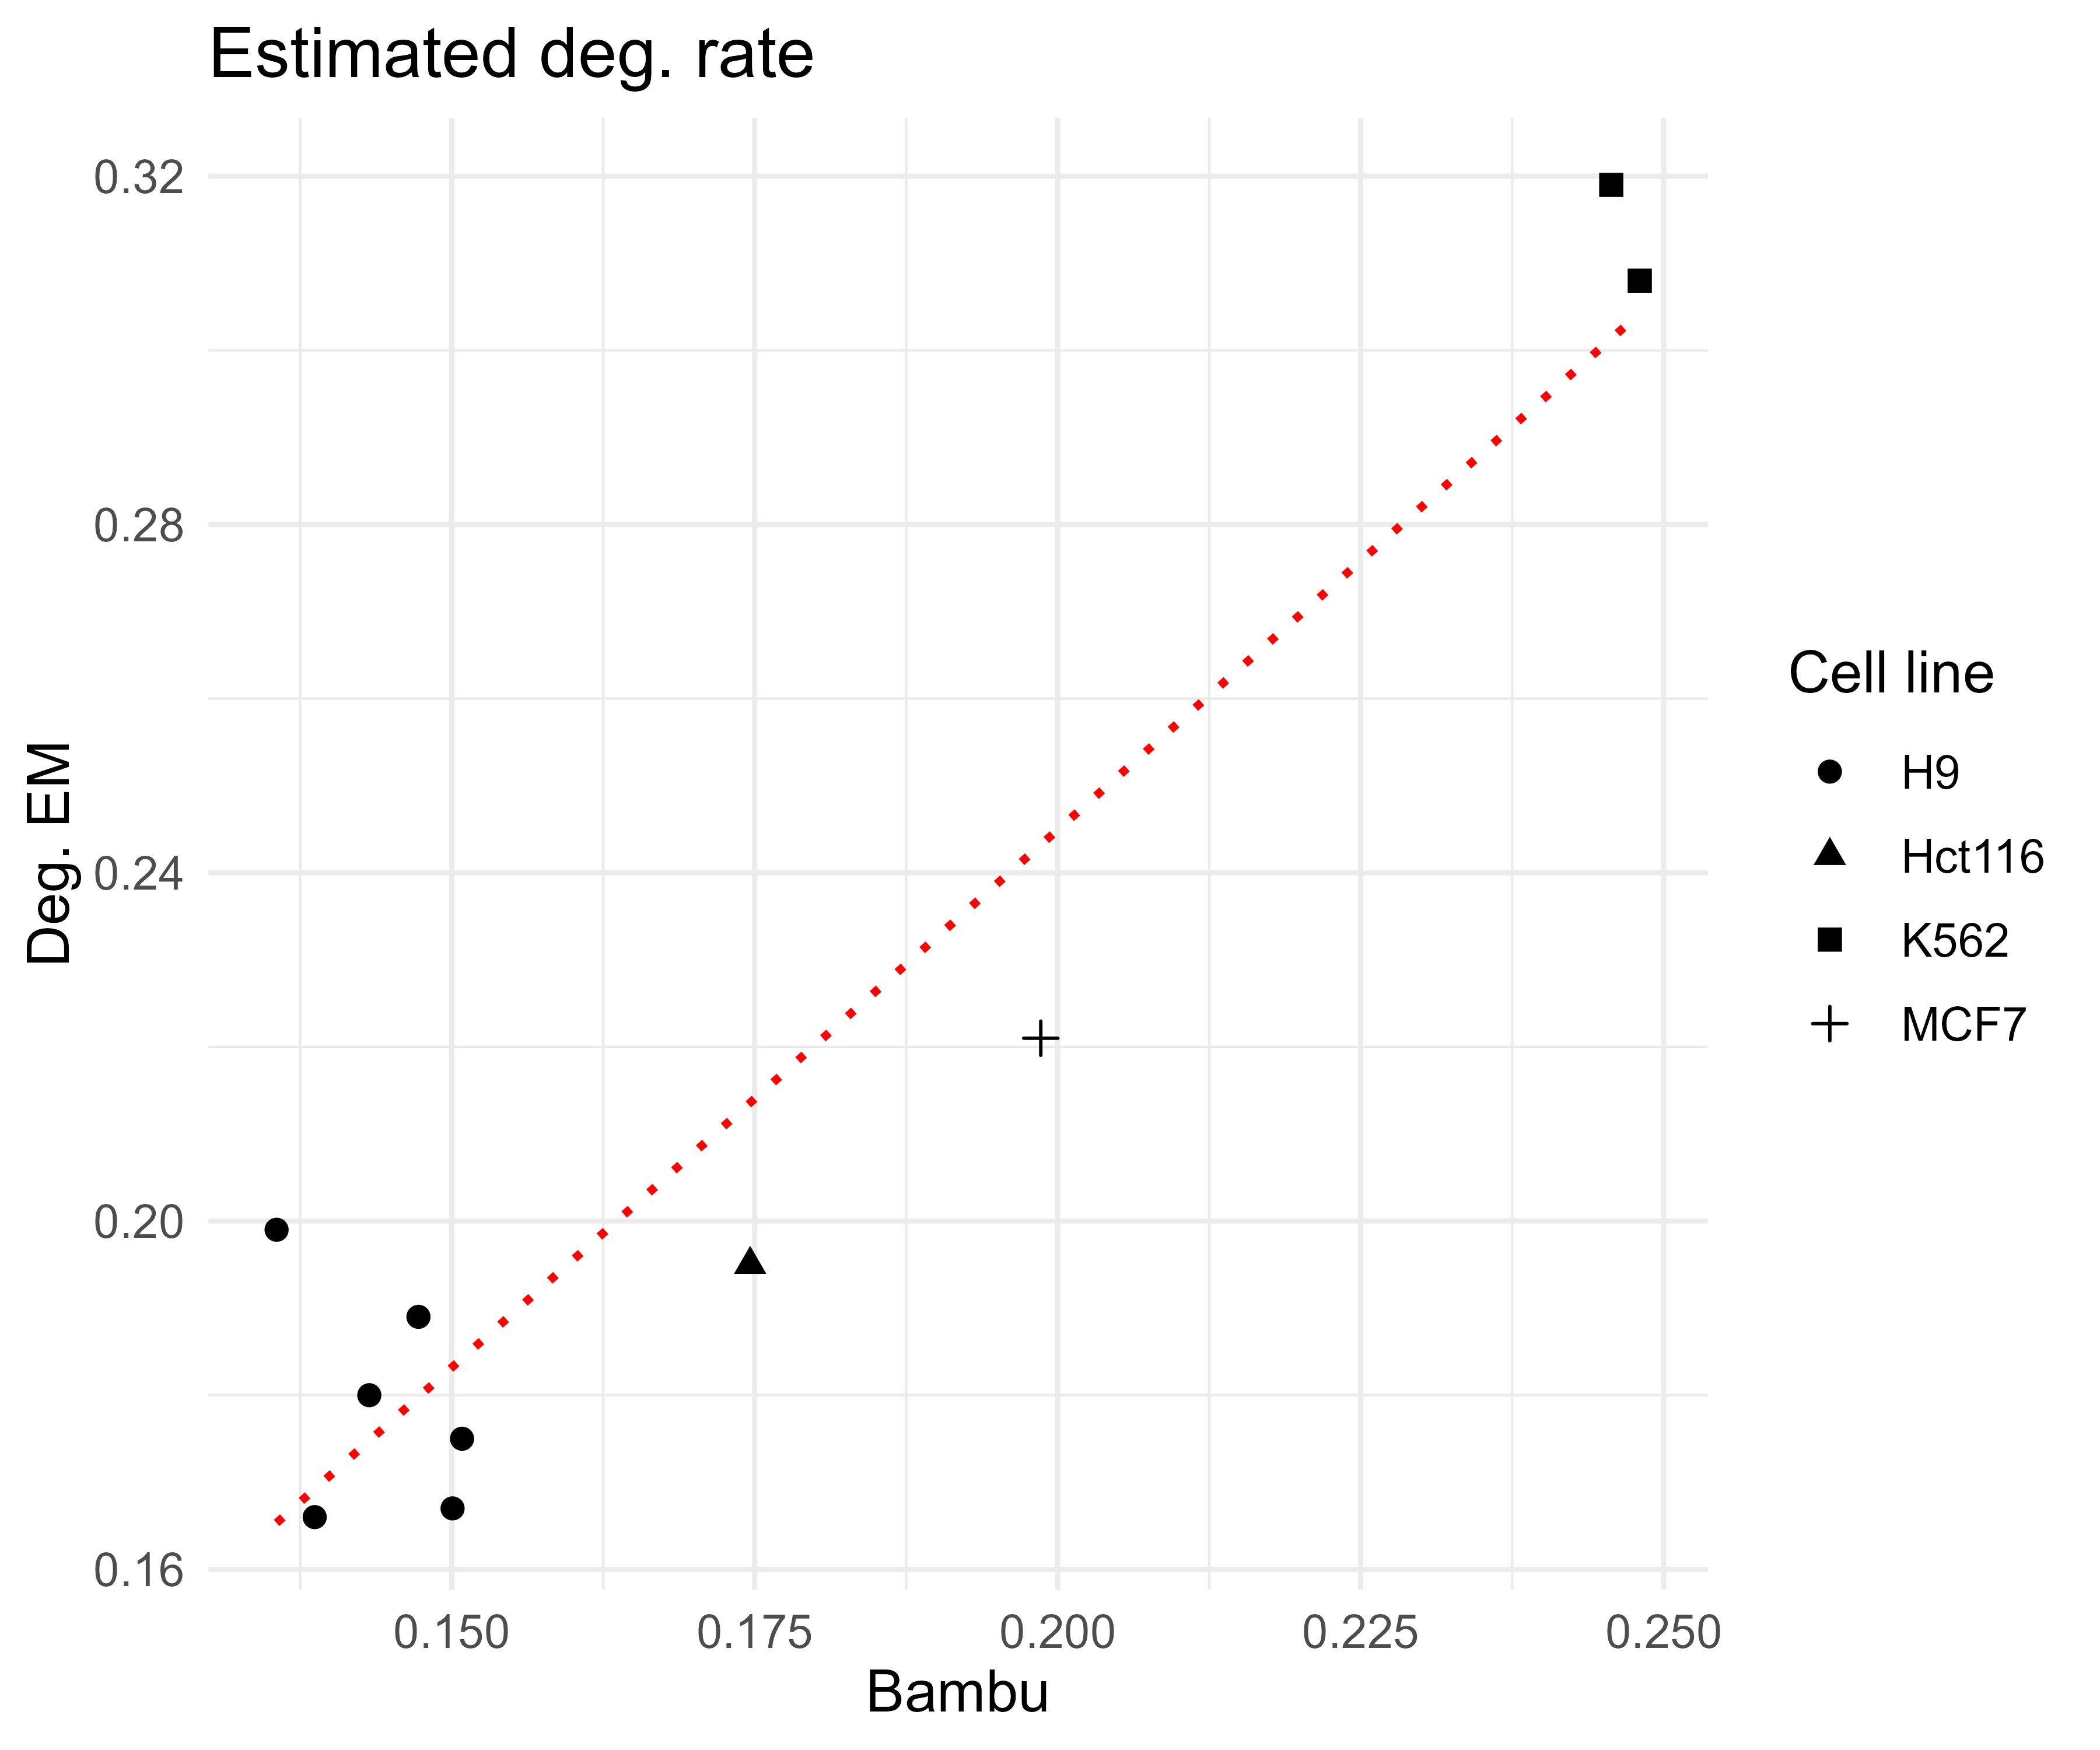
\includegraphics[width=0.65\textwidth]{figures/real-deg-rate.png}
    \caption[Comparison of estimated degradation rates on SG-NEx data]{Comparison of estimated degradation rates on SG-NEx data across four cell lines.}
    \label{fig:real-deg-rate}
\end{figure}


\chapter{Conclusion}

\section{Summary}

In this thesis, we examined degradation bias in long-read direct RNA-seq. We first characterised degradation by formalising the notion of the degradation rate, and estimated degradation rates across different human cell lines. We showed that degradation rates are consistent across isoforms, transcript features and remarkably, sequencing spike-ins. Next, we developed a bias-aware model for transcript quantification that models the probability of observing a read originating from an isoform based on a read length-isoform agreement model. We derive expectation maximization and variational Bayesian inference algorithms for inferring degradation-aware isoform abundance estimates. To evaluate our model, we perform benchmarking against existing methods for transcript quantification. On simulated datasets, our model outperforms other methods on both reference and subset isoforms. On real datasets with sequencing spike-ins, our model achieves results of comparable accuracy to those of existing methods. 

\section{Further work}

To conclude, we highlight three areas of future work.

\subsection{Gene-specific degradation}

Currently, our bias model fits the degradation rate per base globally, with the assumption being that for all isoforms, the degradation rate per base is the same. The validity of this assumption depends on the source of the degradation - if the degradation is mostly a product of RNA decay \textit{in vivo}, then this assumption is unlikely to hold, since differential rates of RNA decay have been extensively described in (cite mrna different decay rates). However, if the degradation is mostly an artifact of the library preparation or sequencing, then a global degradation rate may apply across the isoforms. Nevertheless, it might still be of interest to fit \textit{gene-level degradation rates}, as this would likely improve the accuracy of abundance estimates and reflect the underlying biology more faithfully. 

\subsection{Unobserved degradation}

While we characterised degradation from the data via the read length distribution of the \textit{observed} degraded reads, it is possible that through the entire process of sequencing, transcripts or reads from shorter isoforms would have been fully degraded. This would lead to an underestimation of the counts for short isoforms, and possibly warrant some form of length normalisation for the data. Developing experiments to examine degradation over the course of a sequencing experiment for modeling \textit{unobserved degraded reads} is one potential area of future work.  

\subsection{Read position-isoform agreement}

To model bias, we introduced the read length-isoform agreement, which models the probability of observing a read of a certain length originating from an isoform and its degradation rate. Our current model applies however only to direct RNA-seq, as we assume that the 3' end of all reads align within a close proximity to the annotated 3' end of the isoform. However, it is well known that annotations at both the 5' and 3' end are not clearly well-defined and unreliable. In addition, for direct cDNA and PCR-cDNA protocols, a fraction of reads may not align at the 3' end, resulting in an underestimation of the count. To mitigate these issues and generalise our model to cDNA protocols, we can consider a \textit{read position-isoform agreement} that models the probability of observing a read at a certain start/end position within the sequence of an isoform. 




\appendix
\titleformat{\chapter}[display]
  {\normalfont\huge\bfseries}% <- font for label "Appendix A", default \huge
  {\chaptertitlename\ \thechapter}
  {20pt}
  {\Large}% <- font for title, default \Huge

\chapter{Generating novel isoform models}

In this appendix, we describe our approach for generating novel gene isoform models. As a supplement, we also describe an experimental generative approach developed along the course of this work.   

\section{Modifications from reference isoforms}

To generate novel isoform models, we select a set of seed reference isoforms and introduce modifications that are well known to occur via alternative isoform regulation \textit{in vivo}. These modifications include the use of alternative 5' start sites, alternative 3' end sites, alternative splice donors and acceptors, exon skipping, intron retention, and the introduction of new exons and introns. In addition, we also introduce a new modification, termed \textit{subset} isoform, that drops exons from the reference isoform from the 5' end. Introduction of these novel subset isoforms increases the number of multi-mapping reads, making the process of assigning these reads to the correct isoform more complex. 

%<Insert figure here describing novel isoform models>

Because the \texttt{minimap2} aligner uses splice site signals to map reads, we ensure that the generated novel isoform models conform to these splice site signals. We do so by performing splice site correction whenever necessary, i.e., for the alternative splice donor, alternative splice acceptor, new exon and new intron modifications. 

%<Insert figure here showing splice site correction>

Software for generating novel isoform models was written in \texttt{python} and can be found at \url{https://github.com/jleechung/}.

\section{Generative adversarial modeling}

While the approach detailed above provides precise control over the novel isoform models generated, the resultant models may not be 'biologically' realistic.  

\chapter{Simulating degraded reads}

In this appendix, we describe our approach for simulating reads based on constant expected degradation.

\chapter{Proof of concavity of log-likelihood function}\label{sec:proof-log-lik}

\lipsum[77]

\chapter{Derivations for variational distributions}\label{sec:variational-dist}

\begin{equation}
\begin{split}
    \log q(\bm{Z}) & = \mathbb{E}_{\bm\theta}\left[\log p(\bm{R},\bm{Z},\bm{\theta})\right] + \textrm{const.} \\
    & = \mathbb{E}_{\bm\theta}\left[\log p(\bm{R}\mid\bm{Z})\right] + \mathbb{E}_{\bm\theta}\left[\log p(\bm{Z}\mid\bm{\theta})\right] + \textrm{const.} \\
    & = \sum_i\sum_j z_{ij}\log\left[a_{ij}\cdot p(\ell_i\mid d_j,z_{ij}=1)\right] + \sum_i\sum_j z_{ij}\mathbb{E}_{\bm\theta}\left[\log\theta_j\right] + \textrm{const.}
\end{split}
\end{equation}

\chapter{Evaluation metrics}

\lipsum[32]

\printbibliography[heading=bibintoc]

\end{document}
